
\chapter{Estimating the gas distribution in AGN nuclei} \label{ch:gas_distribution}

\begin{center}
  {\it The work in this Chapter is part of the analysis presented in a paper by Andonie et al., submitted to the Astrophysical Journal.}
  \vspace{1cm}
\end{center}


\section{Introduction}
X-ray emission is a universal characteristic of Active Galactic Nuclei (AGN), thought to arise from inverse Compton upscattering of optical/UV photons of the accretion disk by hot electrons in the corona  \citep[e.g.,][]{1991ApJ...380L..51H}. The intrinsic X-ray emission takes a power-law spectral form  [$f(E){\propto}E^{-\Gamma}$, with  typical photon indices of ${\langle}\Gamma{\rangle}{\sim}1.8$--$2.0$; e.g., \citealt{1994MNRAS.268..405N, 2009ApJ...690.1322W, 2011A&A...530A..42C}], but can be modified due to interaction with matter in the vicinity of the central Supermassive Black Hole (SMBH). In particular, Compton scattering and photoelectric absorption of the primary X-ray continuum lead to two important features in the X-ray spectrum: the \kalfa{} emission line and the so-called "Compton-hump". By studying these reprocessed features, together known as the so-called AGN "reflection" component, we can infer the physical properties of the matter from which they originate, and hence probe the circumnuclear environments of central SMBHs. These physical emissions have to be studied through spectral analysis, as X-ray data do not have enough resolution to allow us to directly observe the very small $\sim pc$ scales where these processes take place, so an indirect approach is needed.

The \kalfa{} line at 6.4 keV is produced by fluorescence processes related to the absorption of higher energy X-ray photons by neutral Fe atoms. Its spectral profile is generally comprised of broad and narrow components. The narrow component of the \kalfa{} line \citep[
$\rm FWHM {\lesssim} 10,000\:km\:s^{-1}$; e.g.,][]{2001MNRAS.323L..37L,2004ApJ...604...63Y,2010ApJS..187..581S} is an ubiquitous spectral feature of AGN, and in a majority of cases the only component present, while the broad component is harder to pin down since it requires exceptional statistics and broad energy coverage to decouple the line from the underlying continuum and absorption components \citep[e.g.,][]{2006AN....327.1032G, 2014ApJ...787...83M}.
Nonetheless, when present, reverberation studies suggest that the broad component originates from a compact zone, only a few $r_g$ in extent, around the SMBH \citep[e.g.,][]{2014MNRAS.438.2980C}, and hence is strongly affected by Doppler and gravitational broadening \citep[e.g.,][]{1995MNRAS.272L...9M,1995Natur.375..659T,1995ApJ...453L..81Y}. On the other hand, the narrow component is thought to be produced somewhere among the outer accretion disk, the broad line region (BLR) and the torus clouds \citep[e.g.,][]{1994MNRAS.267..743G,1994ApJ...420L..57K,1995ApJ...453L..81Y}, corresponding to light month-to-year distances. 

Rapid X-ray continuum variability is commonly observed in unobscured, obscured, and even some heavily obscured AGN and suggests that the primary X-ray emitting source (i.e., the corona) is produced in a compact zone very near to the SMBH \citep[e.g.,][]{1993ARA&A..31..717M, 2013MNRAS.431.2441D}. The X-ray light curve can be analyzed via the power spectral density (PSD) function, which is typically characterized as a power law of the form $P_{\nu} \propto \nu ^{\alpha}$, where $\nu = 1/T$ is the frequency and $\alpha$ is the power law slope \citep[e.g.,][]{1993MNRAS.265..664G, 1999ApJ...514..682E, 2003MNRAS.339.1237V}. Typical values for the power law slope in AGN are $\alpha{\sim}{-}1$ at lower frequencies, indicative of pink noise, and $\alpha\gtrsim-2$ at higher frequencies, indicative of red noise. The break in the PSD between these two regimes is denoted as $\nu_B = 1/T_B$, and is related to the characteristic X-ray variability timescales of the system. 

If we assume that the \kalfa{} line emission is reprocessed from the same X-ray continuum we observe, we can expect the \kalfa{} line flux tracks the continuum fluctuations. The light curves of both, primary and reflected components, can still differ by light travel time effects, as the reflected light can travel different and in general longer paths to the observer. The \kalfa{} line light curve can therefore be delayed with respect to the continuum and can also be smoothed out, as variations on timescales shorter than the light crossing time of the reflector are damped. The reduction of variability amplitude of the \kalfa{} line light curve with respect to the continuum, however, can shed light on the size of the reflector, as larger reflectors suppress a larger fraction of the intrinsic variance. The aim of this Chapter is to take advantage of this correlation between primary and reflected component by using temporal considerations and the variability properties to measure the size of the reflector. We did so in a sample of AGN from the work of Andonie et al. (subm.) by simulating X-ray light curves and comparing their reduction in variability amplitude with the observed ones.

\section{Sample and data}
The AGN sample in this Chapter was presented in Carolina Andonie's master thesis. Onto this same sample we are performing an additional work which will be presented in Andonie et al. (in prep.). The sample was chosen to study the spectral and temporal properties of the \kalfa{} line in AGN, and was selected from the parent input sample the most recent 105-month \textit{Swift}-Burst Alert Telescope (BAT) Survey \citep{2018ApJS..235....4O}, an all-sky survey in the ultra-hard X-ray band (14--195 keV), which provides a relatively unbiased AGN sample at least up to $N_{\rm H}{\gtrsim}10^{24}\:cm^{-2}$ \citep{2015ApJ...815L..13R}. The 105-month Swift-BAT catalog is a uniform hard X-ray all-sky survey with a sensitivity of $8.4 {\times} 10^{-12}\: {\rm erg\:s^{-1}\:cm^{-2}}$ over $90\%$ of the sky in the 14–195 keV band. The survey catalogs 1632 hard X-ray sources, 947 of which are securely classified as AGN but the sample is reduced in order to include only sources with enough multiple observations from either Chandra or XMM. They include one additional target in their sample, the well-known narrow-line Sy1 1H0707$-$495, which is relatively bright in the 2--8\,keV band, yet somehow remains undetected in the BAT 105-month catalog.

Andonie et al. focus on observations in the 2-8 keV band where the \kalfa{} line is located, and use data from \textit{Chandra} \citep{2000SPIE.4012....2W} and \textit{XMM-Newton} \citep{2001A&A...365L...1J} which have a good sensitivity in this band. \textit{XMM-Newton} observations provide better spectral and timing statistics, but suffer from substantial background flaring.
On the other hand, \textit{Chandra} observations are more versatile since they offer high spatial resolution to search for extended \kalfa{} emission on $\sim$100-pc to kpc scales, and, when the High Energy Grating is deployed, sufficient spectral resolution to resolve the \kalfa{} line.

The authors limit their analysis only to those observations for which there is a high likelihood of constraining the \kalfa{} line, and apply a flux cut of $f_{\rm 14-195\: keV} \geqslant  10^{-11}\: {\rm erg\:s^{-1}\:cm^{-2}}$ and/or $f_{\rm 2-8\: keV} \geqslant  4\times 10^{-12} \: {\rm erg\:s^{-1}\:cm^{-2}}$ (these are roughly equivalent for a $\Gamma{=}1.9$ power law); this resulted in the selection of 252 sources in the local universe ($z<0.1$), and 28 more distant galaxies with redshifts between 0.1 and 0.56.

We simulate X-ray light curves for those galaxies which have determined PSD function parameters from either \citet{summons_thesis}, from long term monitoring campaigns performed with the Rossi X-Ray Timing Explorer (RXTE) observatory, or from \citet{2012A&A...544A..80G} (\citetalias{2012A&A...544A..80G} hereafter), from \emph{XMM-Newton}/pn observations. For the rest, we estimated the break frequency using the expression
\begin{equation}
    \log(T_b)=1.09\log(M_{BH}) + -0.24\log(L_{bol}) - 1.88
    \label{Eq:T_b}
\end{equation}
from \citetalias{2012A&A...544A..80G}, where $T_b$ is the PSD bending timescale ($T_b = 1/\nu_{b}$), $M_{BH}$ is the black hole mass in $10^6\:\rm M_{\odot}$ units, and  $L_{bol}$ is the bolometric luminosity in $10^{44}\:\rm erg\:s^{-1}$ units.

The final sample for which we are able to simulate X-ray light curves is composed of 33 sources which have between 2--68 observations in a time range between $\sim1600-7000$ days. A complete list of the sources, their PSD parameters and observations is reported in Table \ref{tab:gals_obs_par}.

\section{Variability definitions} \label{sec:variability_defs}
The light curves obtained by Andonie el al. are too sparsely sampled to detect a delay between continuum and Fe line fluctuations, therefore we rely on estimating the reduction in variability amplitude. This can be quantified by calculating the ratio between the excess variance of the continuum ($\sigma^2_{\rm ct}$) and \kalfa{} line ($\sigma^2_{\rm Fe}$) light curves, as %$\xi_{r}=\sigma^2_{\rm Fe}/\sigma^2_{\rm ct}$.
\begin{equation}\label{eq:xi}
    \xi_{r}=\frac{\sigma^2_{Fe}}{\sigma^2_{ct}}.
\end{equation}
The normalized excess variance ($\sigma^2$) \citep[e.g.,][]{1997ApJ...476...70N,2004ApJ...611...93P,2008A&A...487..475P} is a quantitative measurement of the variability amplitude of a light curve, and is defined as
\begin{equation}
\label{eq:NXS}
    \sigma^2_{rms} = \frac{1}{N_{obs}\overline{x}^2} \sum^{N_{obs}}_{i=1} [(x_i-\overline{x})^2-\sigma^2_{err,i}]
\end{equation}
while its error due to Poison noise is
\begin{equation}
\label{eq:NXS_err}
 err( \sigma^2_{rms}) = \frac{1}{N_{obs}^{3/2}\overline{x}^2} \sum^{N_{obs}}_{i=1} ([(x_i-\overline{x})^2-\sigma^2_{err,i}]-\sigma^2_{rms} \overline{x}^2)^2\,.
\end{equation}
The $\sigma^2_{rms}$ estimates the intrinsic variance of the light curve, normalized by its mean flux, to produce a dimensionless quantifier that can be easily compared between objects of different brightness or light curves from  different energy bands. The last term in Eq.~\ref{eq:NXS} estimates the contribution of the observational Poisson noise to the total variance, in order to subtract it, and the error formula in Eq.~\ref{eq:NXS_err} estimates the uncertainty in this subtraction. 

The excess variances and their ratios were estimated by running Monte Carlo simulations in order to quantify their variability robustly. 
These simulations are only aimed at quantifying how the observational Poisson noise affects the estimate of the $\sigma^2_{rms}$. For this purpose we add Gaussian noise to each light curve point, with a $\sigma$ equal to the error on the flux of each point. In this way, each simulation has the intrinsic variance of the light curve and twice the observational noise and allows to estimate the excess variance and its asymmetric uncertainties for each light curve.

Low intrinsic variances compared to the Poisson noise can sometimes lead to negative values of the $\sigma^2_{rms}$ estimate, since the uncertainty in the Poisson noise can be larger than the difference in Eq.~\ref{eq:NXS}. We will consider light curves as significantly variable if the lower 16\% bound of the excess variance distribution is positive. Table \ref{tab:gals_obs_par} shows the median and the 16\% and 84\% bounds of the ratio distributions of the excess variance of each light curve. These data are also plotted in Fig.~\ref{fig:exvars}. 

Significant variability (i.e. positive lower bound on the $\sigma^2_{rms}$ ) is detected in the continuum of all objects except for 4C+29.30.  Significant Fe K$\alpha$ line variability is detected in 2MASXJ23444387, 4C+74.26, Cen A, Circinus galaxy, IC4329A, MR2251-178, MRK 1040, MRK 1210, MRK 3, NGC 1068, NGC 1275, NGC 1365, NGC 253, NGC 2992, NGC 3783, NGC 4151, NGC 4388, NGC 6300 and NGC 7582. In many objects, however, the variability of the Fe K$\alpha$ line is consistent with the observational noise, within its uncertainties. This is the case for all objects for which the lower bound on the Fe K$\alpha$ line excess variance is negative. The upper bounds on the Fe K$\alpha$ line variability in those objects is still of interest, depending on how this bound compares to the variance of the continuum.

If the Fe K$\alpha$ line flux tracks the fluctuations of the continuum flux, then we expect their variances to be related. The ratio of the variances $\xi$ should be similar to 1 if the reflector is small compared to the timescale of the fluctuations, and smaller than 1 if the reflector is large. Therefore, upper bounds smaller than 1 in the ratio column of Table~\ref{tab:gals_obs_par} can allow us to place a lower limit on the size of the reflector. This is true for example in the first two objects in the table. Even though their Fe K$\alpha$ line variance is not significant, its upper limit is so far below the variance of the continuum that a lower limit can be placed on the size of the reflector, because if the reflector was any smaller, the Fe K$\alpha$ line variability would be detectable. Conversely, lower bounds of the variance ratio $\xi>0$ can put upper limits on the reflector size. One or both of these limits are therefore measurable in many objects in the table. We describe this analysis below in Sec.~\ref{sec:LC_sims}.

%The normalized excess variance of the continuum is generally well constrained. The median values of the $\sigma^2_{rms}$ distributions range from 0.006 for 3C 445 to 9.99 for 2MASXJ11315154-1231587. This large difference can raise doubts about a common origin of the continuum variability in all sources. We know however, from dedicated monitoring campaigns of radio-quiet AGN, that the X-ray power spectra of different AGN is remarkably uniform in shape and normalization, but that the timescale of the break in the power spectrum scales linearly with black hole mass and and inversely with accretion rate \citep{2006Natur.444..730M}. Since the excess variance equals the integral of the power spectrum over the timescales covered by the light curves, we can expect to measure significantly different values for objects of different black hole mass, even if the light curves have similar lengths.  

%To test how unusual some of these excess variances are, we computed the expected variance, for the respective BH masses and accretion rates. Since the variability is a stochastic process, and the underlying powerspectral shape is only realized on average, simulations provide a good way of estimating the possible range of variance measurements, for given BH parameters and light curve sampling pattern. 

\begin{figure*} 
 \centering
 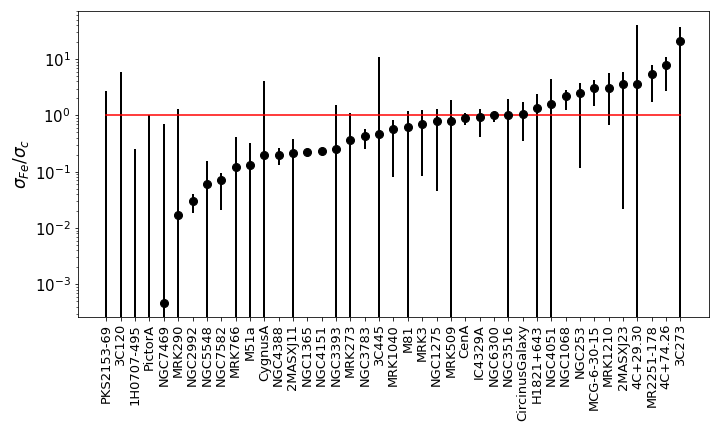
\includegraphics[width=\textwidth]{Figs/Chapter5/ratio_1s.png}
 %\captionsetup{width=1.5\linewidth}  
 \caption{The ratio between the normalized excess variance of the Fe K$\alpha$ line and continuum light curves $\xi=\sigma_{Fe}/\sigma_{ct}$. The error bars correspond to the 16$\%$ and 84$\%$ bounds of the normalized excess variance distributions.}\label{fig:exvars}
 \end{figure*} 

% USEFUL COMMENTS, DO NOT ERASE:
%Source                 & $\xi(50\%)_{16\%}^{84\%}$        & $\log{\rm M}_{\rm BH}$ & $\log L_{bol}$& $\nu_b$ & $\nu_b$  & $\alpha_h$ & Ref. & N Obs & Duration\\
%                       &              & $(\rm M_\odot)$ & (erg/s) & (Hz)    & (days$^{-1}$) & & & & (days) \\
% \caption{The galaxy sample from Andonie et al. (in prep.), its observations and its PSD parameters. Median $\xi$ parameters are reported with the 16\% to 84\% bounds of the distributions of normalized excess variance. Black hole masses are from Bass collaboration. $\nu_b$ and $\alpha_h$ (if available) are shown with the work they was extracted from and, whenever not available, the $\nu_b$ estimation with Eq.~\ref{Eq:T_b} is shown.}\label{tab:gals_obs_par}
%\specialcell{2MASXJ11315154\\-1231587}
\begin{footnotesize}%small
\begin{longtable}{llrrllrlrr}
\toprule
Source                 & $\xi(50\%)_{16\%}^{84\%}$        & $\log{\rm M}_{\rm BH}$ & $\log L_{bol}$& $\nu_b$ & $\nu_b$  & $\alpha_h$ & Ref. & N Obs & Duration\\
                       &              & $(\rm M_\odot)$ & (erg/s) & (Hz)    & (days$^{-1}$) & & & & (days) \\
\midrule
\endhead
\midrule
\multicolumn{10}{r}{{Continued on next page}} \\
\midrule
\endfoot

%\bottomrule
\endlastfoot
1H0707-495             &   $ -0.18_{-0.82}^{0.28} $ &             - &       - & $3.98\cdot10^{-4}$ &          34. &      2.4 &  {\citetalias{2012A&A...544A..80G}} &    14 &     6929 \\
\specialcell{2MASXJ11315154\\-1231587} &   $ 0.20_{-0.026}^{0.39} $ &          8.81 &    46.6 & $6.22\cdot10^{-7}$ &        0.054 &        - &                    Eq.~\ref{Eq:T_b} &    41 &     4990 \\
3C120                  &      $ -1.3_{-19.}^{6.6} $ &          7.74 &    45.2 & $7.83\cdot10^{-6}$ &         0.68 &        - &                    Eq.~\ref{Eq:T_b} &    11 &     4879 \\
3C273                  &       $ 18._{-17.}^{36.} $ &          8.84 &    47.0 & $7.30\cdot10^{-7}$ &        0.063 &        - &                    Eq.~\ref{Eq:T_b} &    47 &     6595 \\
4C+29.30               &       $ 3.8_{-27.}^{40.} $ &          8.28 &    44.9 & $1.28\cdot10^{-6}$ &         0.11 &        - &                    Eq.~\ref{Eq:T_b} &     6 &     3245 \\
4C+74.26               &        $ 7.7_{2.1}^{11.} $ &          9.83 &    46.0 & $2.00\cdot10^{-8}$ &       0.0017 &        - &                    Eq.~\ref{Eq:T_b} &     6 &     1571 \\
CenA                   &      $ 0.92_{0.66}^{1.1} $ &          7.77 &    43.1 & $2.26\cdot10^{-6}$ &         0.20 &        - &                    Eq.~\ref{Eq:T_b} &    39 &     6581 \\
CircinusGalaxy         &       $ 1.1_{0.33}^{1.8} $ &          6.23 &    43.5 & $1.07\cdot10^{-4}$ &          9.3 &      2.1 &  {\citetalias{2012A&A...544A..80G}} &    18 &     5006 \\
CygnusA                &     $ -0.51_{-6.0}^{3.7} $ &          9.43 &    45.6 & $5.30\cdot10^{-8}$ &       0.0046 &        - &                    Eq.~\ref{Eq:T_b} &    68 &     6209 \\
IC4329A                &      $ 0.99_{0.47}^{1.3} $ &          7.81 &    45.0 & $5.85\cdot10^{-6}$ &         0.51 &        - &                    Eq.~\ref{Eq:T_b} &    13 &     6222 \\
M81                    &     $ 0.75_{-0.24}^{1.2} $ &          7.90 &    39.5 & $2.13\cdot10^{-7}$ &        0.018 &        - &                    Eq.~\ref{Eq:T_b} &    38 &     6157 \\
MCG-6-30-15            &        $ 3.0_{1.5}^{4.2} $ &          6.14 &    43.9 & $3.80\cdot10^{-5}$ &          3.3 &      1.9 &            {\citet{summons_thesis}} &    12 &     4589 \\
MR2251-178             &        $ 5.3_{2.0}^{7.9} $ &          8.20 &    45.8 & $2.50\cdot10^{-7}$ &        0.022 &      2.5 &            {\citet{summons_thesis}} &    12 &     5489 \\
MRK1040                &     $ 0.57_{0.18}^{0.82} $ &          7.41 &    44.6 & $1.55\cdot10^{-5}$ &          1.3 &        - &                    Eq.~\ref{Eq:T_b} &     8 &     4770 \\
MRK1210                &       $ 3.4_{0.90}^{6.1} $ &          6.76 &    44.3 & $9.94\cdot10^{-5}$ &          8.6 &        - &                    Eq.~\ref{Eq:T_b} &     7 &     2496 \\
MRK273                 &     $ 0.43_{-0.90}^{1.0} $ &          8.78 &    44.1 & $1.78\cdot10^{-7}$ &        0.015 &        - &                    Eq.~\ref{Eq:T_b} &     8 &     6149 \\
MRK290                 &      $ 0.13_{-1.7}^{1.4} $ &          7.28 &    44.4 & $2.06\cdot10^{-5}$ &          1.8 &        - &                    Eq.~\ref{Eq:T_b} &     8 &     1042 \\
MRK3                   &      $ 0.73_{0.12}^{1.3} $ &          6.72 &    44.8 & $1.51\cdot10^{-4}$ &          13. &        - &                    Eq.~\ref{Eq:T_b} &    19 &     5511 \\
MRK509                 &     $ 0.76_{-0.81}^{1.8} $ &          8.05 &    45.3 & $7.60\cdot10^{-8}$ &       0.0066 &      1.5 &            {\citet{summons_thesis}} &    18 &     4335 \\
MRK766                 &    $ 0.11_{-0.35}^{0.43} $ &          6.60 &    43.9 & $2.90\cdot10^{-4}$ &          25. &      2.9 &            {\citet{summons_thesis}} &    11 &     5172 \\
NGC1068                &        $ 2.3_{1.4}^{2.8} $ &          6.93 &    43.9 & $4.81\cdot10^{-5}$ &          4.2 &        - &                    Eq.~\ref{Eq:T_b} &    12 &     5301 \\
NGC1275                &     $ 0.82_{0.025}^{1.3} $ &          7.55 &    45.1 & $1.38\cdot10^{-5}$ &          1.2 &        - &                    Eq.~\ref{Eq:T_b} &    44 &     6650 \\
NGC1365                &     $ 0.22_{0.19}^{0.25} $ &          7.60 &    43.4 & $2.21\cdot10^{-6}$ &         0.19 &        - &                    Eq.~\ref{Eq:T_b} &     9 &     3314 \\
NGC2992                &  $ 0.031_{0.019}^{0.040} $ &          8.33 &    43.1 & $4.09\cdot10^{-7}$ &        0.035 &        - &                    Eq.~\ref{Eq:T_b} &    13 &     3644 \\
NGC3393                &      $ 0.29_{-1.7}^{1.7} $ &          7.52 &    43.8 & $7.24\cdot10^{-6}$ &         0.63 &        - &                    Eq.~\ref{Eq:T_b} &     5 &     3199 \\
NGC3516                &      $ 1.0_{-0.68}^{2.0} $ &          7.39 &    43.9 & $6.60\cdot10^{-6}$ &         0.57 &      2.9 &            {\citet{summons_thesis}} &     9 &     2204 \\
NGC3783                &     $ 0.45_{0.29}^{0.58} $ &          7.37 &    44.6 & $1.30\cdot10^{-5}$ &          1.1 &      2.6 &            {\citet{summons_thesis}} &    13 &     6179 \\
NGC4051                &       $ 1.8_{-3.3}^{4.4} $ &          6.13 &    42.4 & $5.10\cdot10^{-4}$ &          44. &      2.5 &            {\citet{summons_thesis}} &    42 &     5866 \\
NGC4151                &     $ 0.24_{0.22}^{0.25} $ &          7.56 &    43.4 & $2.60\cdot10^{-7}$ &        0.022 &      2.2 &            {\citet{summons_thesis}} &    35 &     5769 \\
NGC4388                &     $ 0.20_{0.13}^{0.26} $ &          6.94 &    44.2 & $5.45\cdot10^{-5}$ &          4.7 &        - &                    Eq.~\ref{Eq:T_b} &     5 &     3267 \\
NGC5548                &  $ 0.042_{-0.071}^{0.15} $ &          7.72 &    44.3 & $1.30\cdot10^{-6}$ &         0.11 &      3.5 &            {\citet{summons_thesis}} &    21 &     5823 \\
NGC6300                &        $ 1.0_{1.0}^{1.1} $ &          6.57 &    43.0 & $8.84\cdot10^{-5}$ &          7.6 &        - &                    Eq.~\ref{Eq:T_b} &     6 &     3026 \\
NGC7469                &   $ -0.036_{-1.2}^{0.68} $ &          6.96 &    44.4 & $5.60\cdot10^{-5}$ &          4.8 &        - &                    Eq.~\ref{Eq:T_b} &    12 &     5480 \\
NGC7582                &  $ 0.070_{0.018}^{0.094} $ &          7.74 &    44.7 & $5.89\cdot10^{-6}$ &         0.51 &        - &                    Eq.~\ref{Eq:T_b} &     7 &     6371 \\
Pictor A                &    $ -0.34_{-3.1}^{0.88} $ &          6.80 &    44.6 & $1.06\cdot10^{-4}$ &          9.1 &        - &                    Eq.~\ref{Eq:T_b} &    17 &     5471 \\
\hline
\caption{The galaxy sample from Andonie et al. (in prep.), its observations and its PSD parameters. Median $\xi$ parameters are reported with the 16\% to 84\% bounds of the distributions of normalized excess variance. Black hole masses and $L_{bol}$ are from BASS DR2 (in prep.). $\nu_b$ and $\alpha_h$ (if available) are shown with the work they was extracted from and, whenever not available, the $\nu_b$ estimation with Eq.~\ref{Eq:T_b} is shown.}\label{tab:gals_obs_par}\\
\end{longtable}
\end{footnotesize}


The longer the light crossing time of the reflector, the smaller the expected value of $\xi_{r}$ is.
Although it is straightforward to estimate $\xi_{r}$ as a function of the break frequency of the continuum light curve power spectrum and the light crossing time of the reflector, we expect a large scatter in measured values of $\xi_{r}$ due to the small number of data points and the stochastic nature of the light curves. We therefore took the Monte Carlo approach described below to place meaningful constraints on the size of the reflector.
 
\section{Light curves simulation}\label{sec:LC_sims}
We simulate light curves following the method of \citet{1995A&A...300..707T}, which consists in simulating white noise in Fourier space, defined as a normally distributed process with a real and imaginary part with a standard deviation that depends on the filter function, our power spectrum. 
We assume a power spectrum with the shape of a bending power law in Fourier space:
\begin{equation}
    PS=\frac{A\nu^{-\alpha_L}}{1+(\nu/\nu_b)^{\alpha_H-\alpha_L}}
\end{equation}
with a low-frequency slope $\alpha_L =1$ bending at higher frequencies to a steeper slope $\alpha_h$ at a characteristic timescale or break frequency $\nu_b$. The normalization was given a value of $A = 0.001$ which conforms to the majority of sources measured in \citet{summons_thesis}. The variance scales linearly with the normalization $A$, so varying $A$ will shift the mean expected variance and its scatter by the same amount. Differences in $A$ by a factor of 2 (higher or lower) are consistent with the monitored sample. When no estimate of a high frequency slope is available from the literature, we assumed $\alpha_H=2$. %$\alpha_l$ and $\nu_b$ are either retrieved from the literature (insert papers) or estimated with Eq. ... from ... by using .... from the BASS collaboration. 

To simulate the corresponding reflected light curves we multiplied the simulated continuum light curve in Fourier space for a $\sinc(\nu\tau)$ function, which corresponds to a top hat filter, and shifted the inverse Fourier transformed curve forward in time by $\tau/2$ days. This simple setup corresponds to the reflection by a spherical thin shell of radius $R=c\tau/2$ and can be viewed as an immediate response of the front end of the reflector, followed by the reflection of the rest of the shell until the light from the back end finally reaches the observer $2R/c=\tau$ days after the start of the response. This particular response function was chosen for simplicity and reproduces the main characteristics of a reflected light curve, which is sufficient to estimate the size, though not the geometry, of the reflector.  

\begin{figure}
\begin{center}
    {
 % \includegraphics[width=0.49\textwidth]{Figs/Chapter5/NGC4151/power_spectrum_tau1.0.pdf}  \hfill
 % 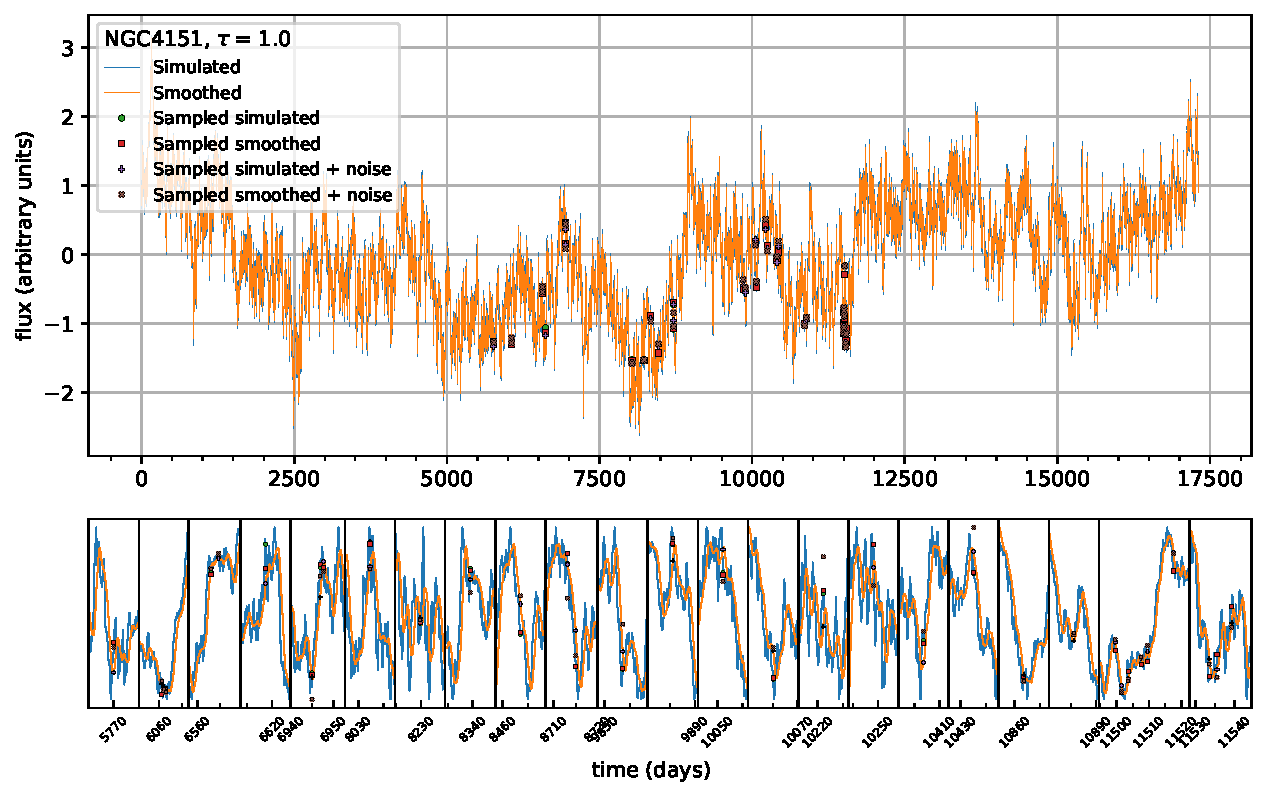
\includegraphics[width=0.49\textwidth]{Figs/Chapter5/NGC4151/sim_LC_tau1.0_0_matrix.pdf} \\
  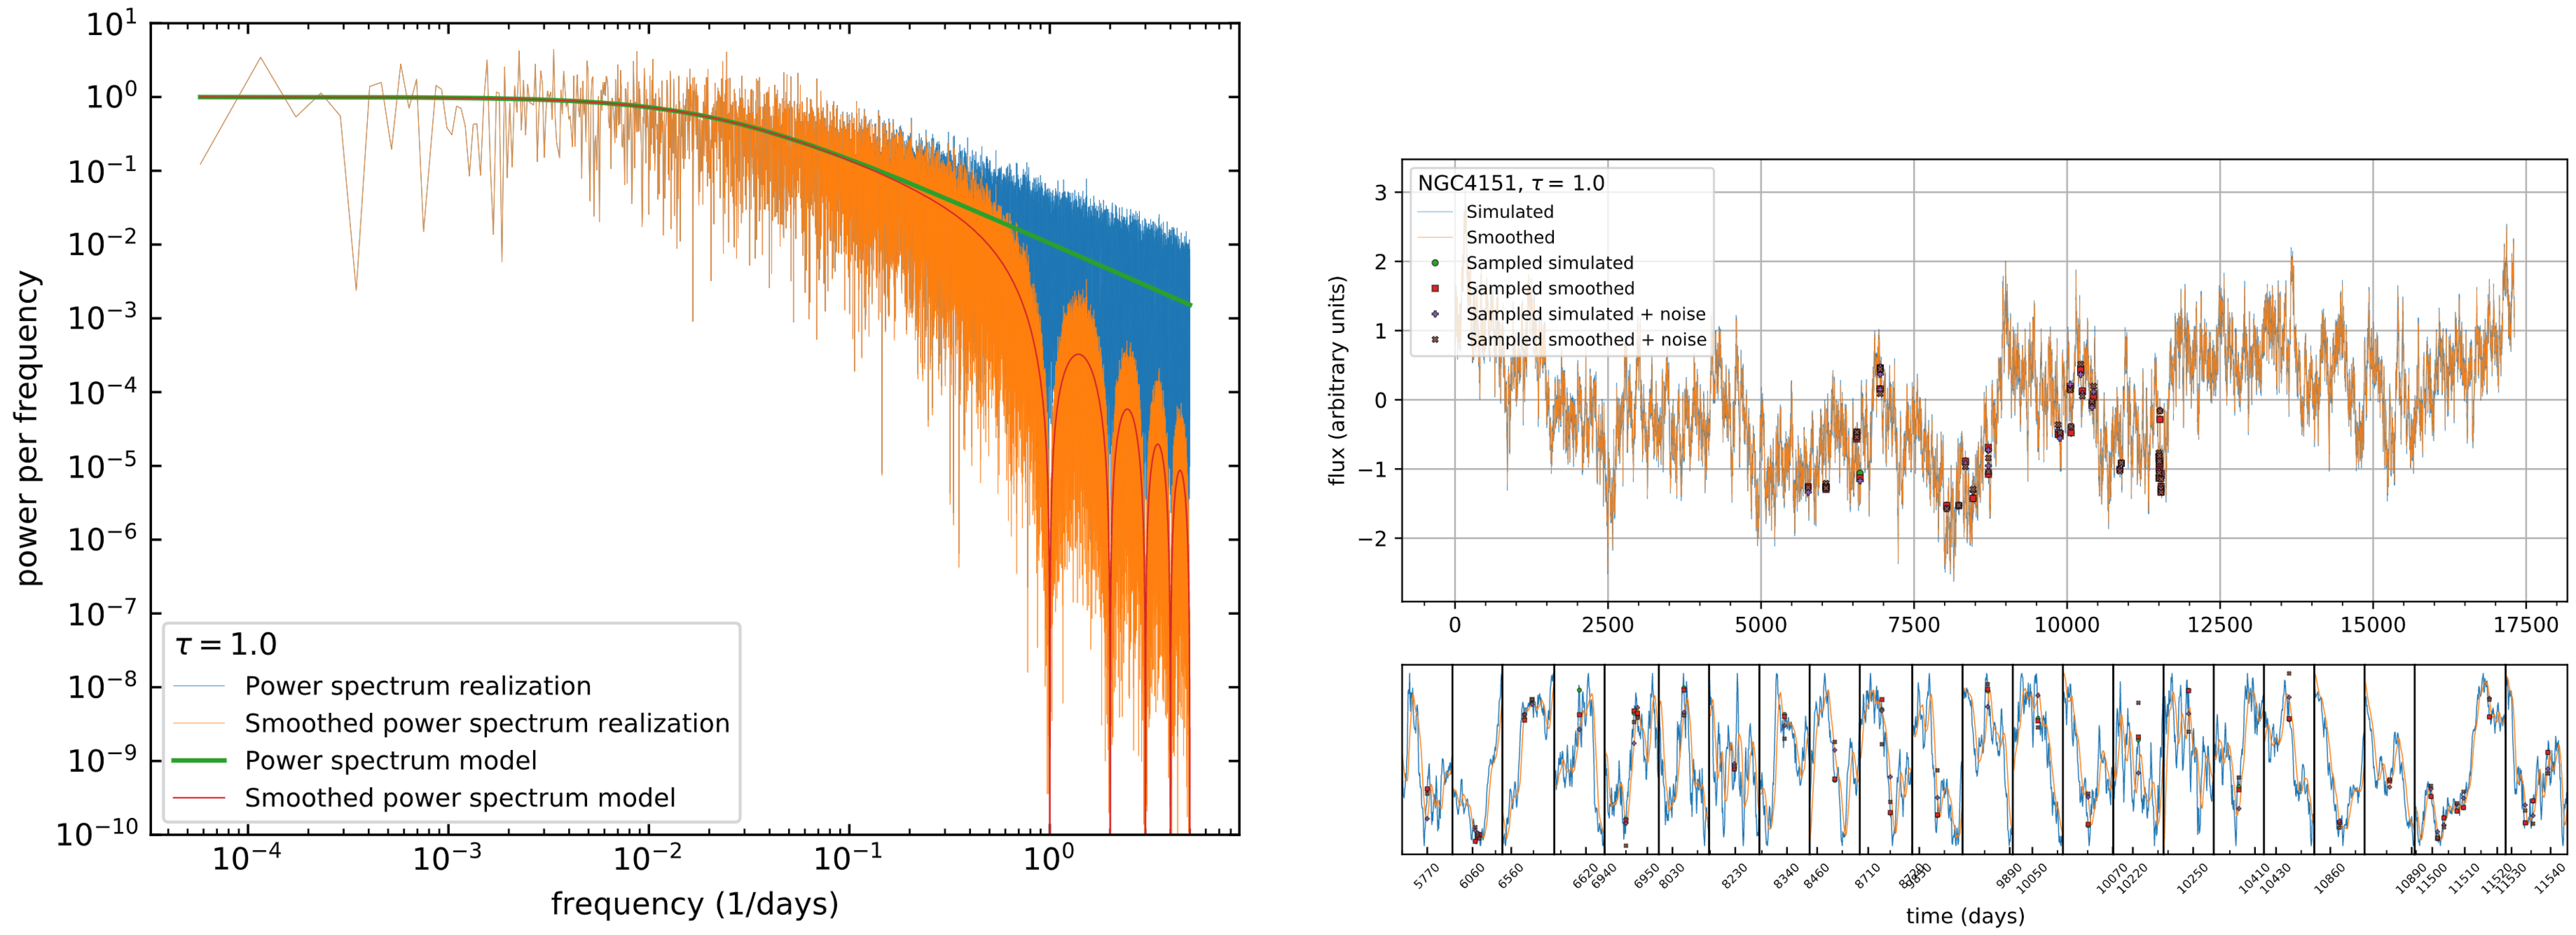
\includegraphics[width=\textwidth]{Figs/Chapter5/NGC4151/Screenshots/NGC4151_tau1_LC_spectrum.pdf} \\
 % 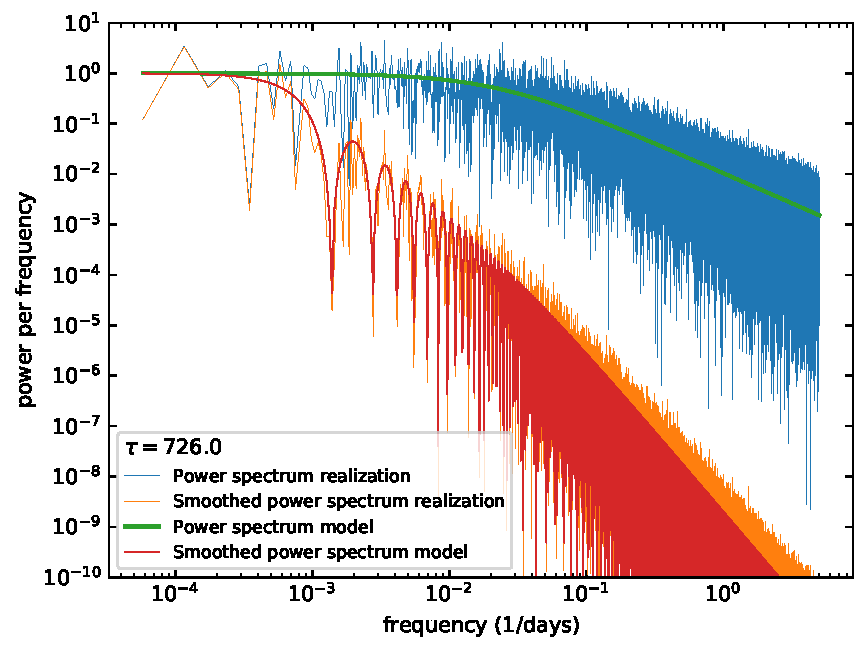
\includegraphics[width=0.49\textwidth]{Figs/Chapter5/NGC4151/power_spectrum_tau726.0.pdf}\hfill 
 % 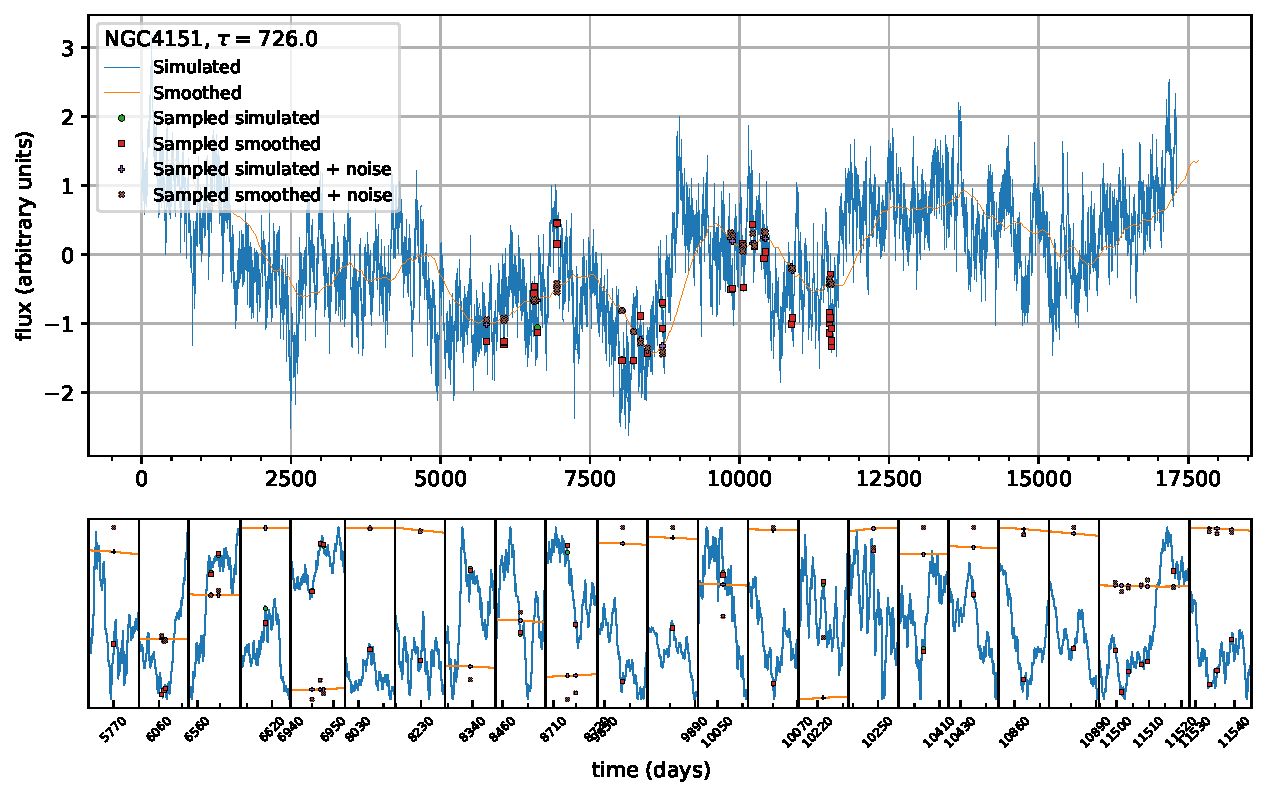
\includegraphics[width=0.49\textwidth]{Figs/Chapter5/NGC4151/sim_LC_tau726.0_0_matrix.pdf} \\
  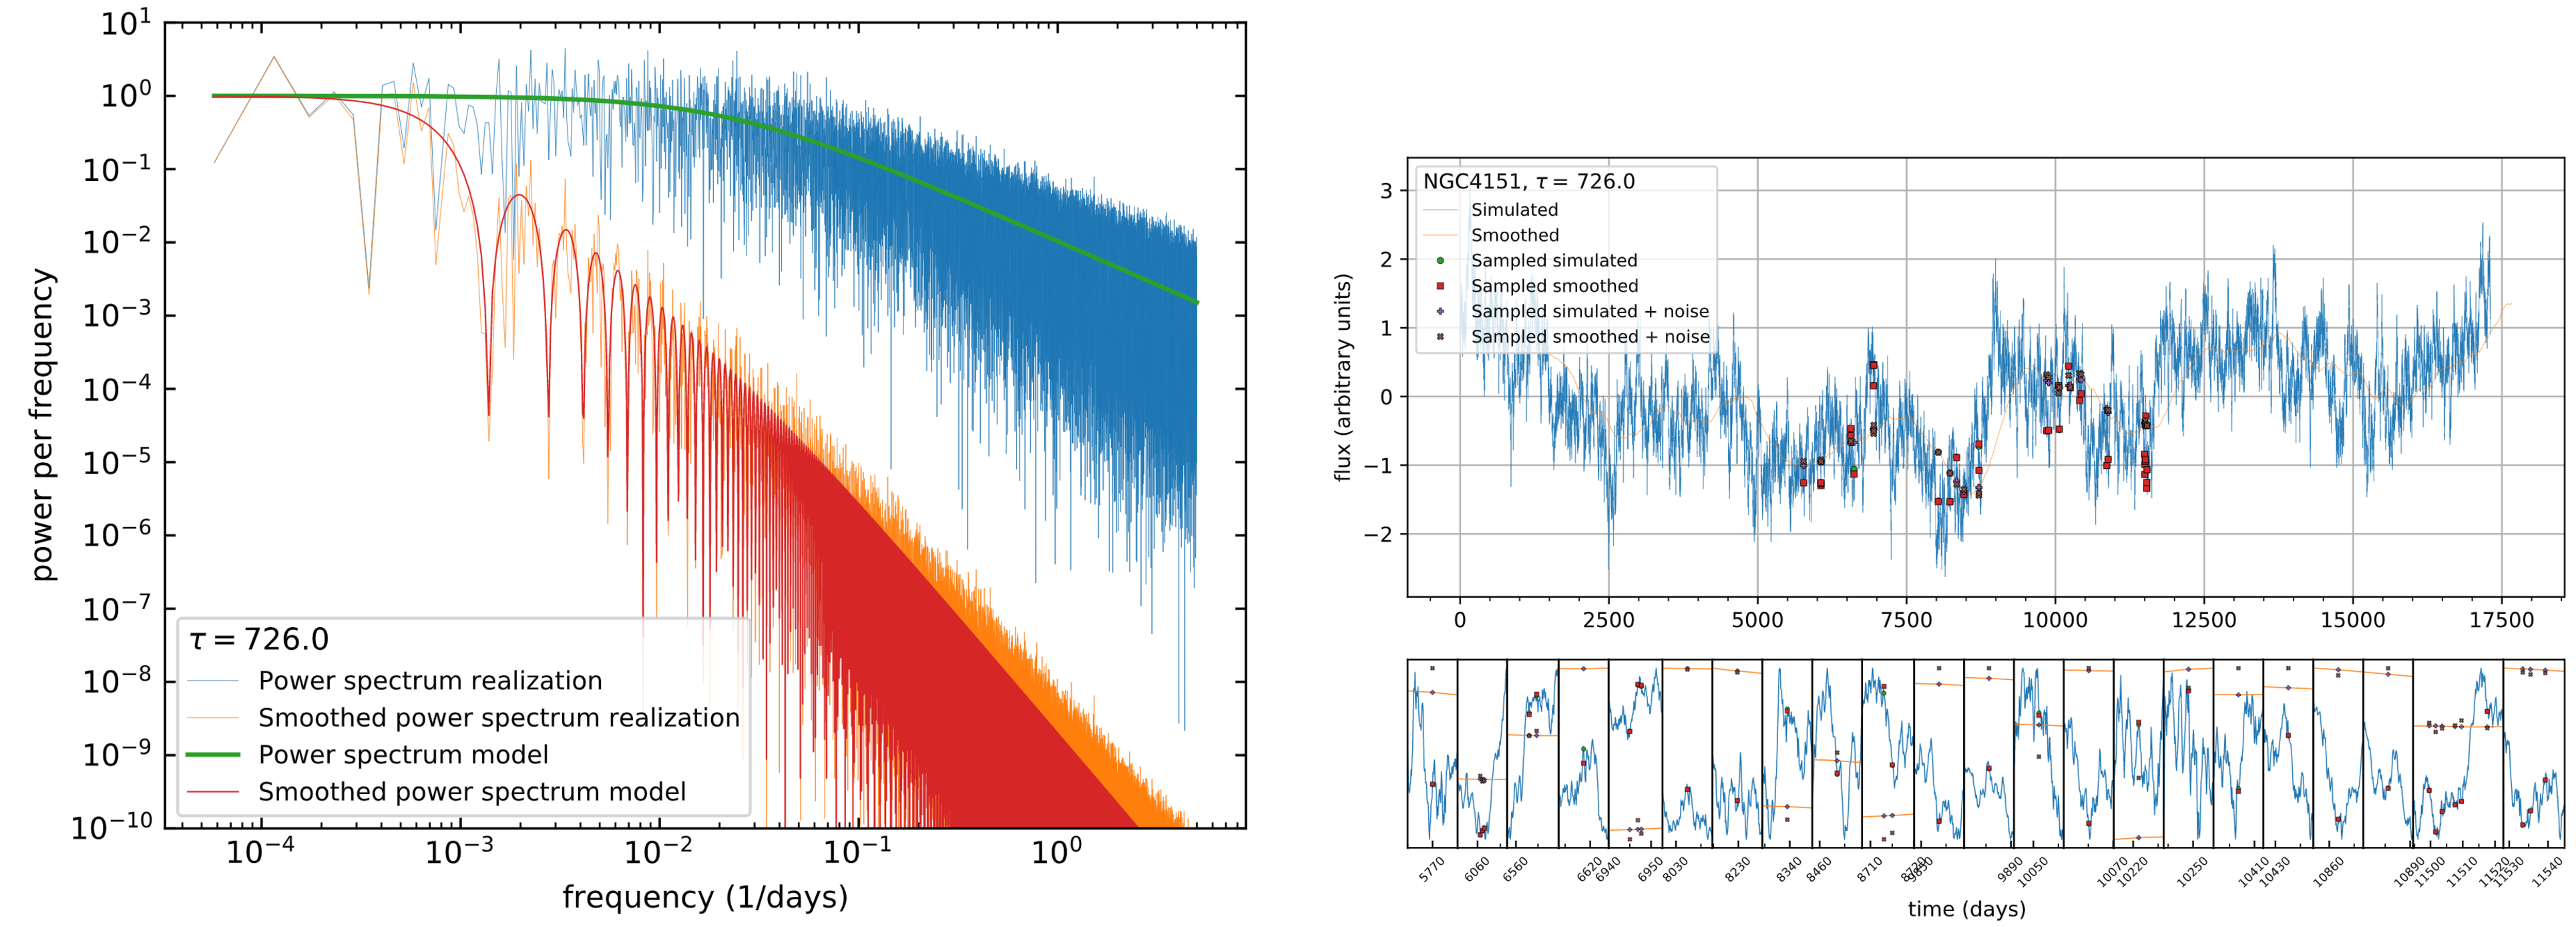
\includegraphics[width=\textwidth]{Figs/Chapter5/NGC4151/Screenshots/NGC4151_tau726_LC_spectrum.pdf} \\
%  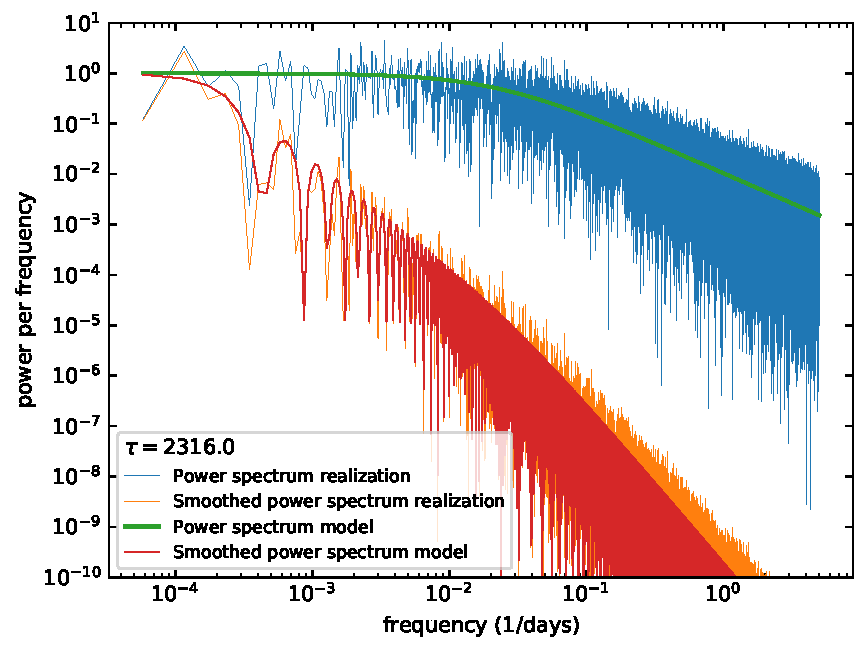
\includegraphics[width=0.49\textwidth]{Figs/Chapter5/NGC4151/power_spectrum_tau2316.0.pdf} \hfill 
%  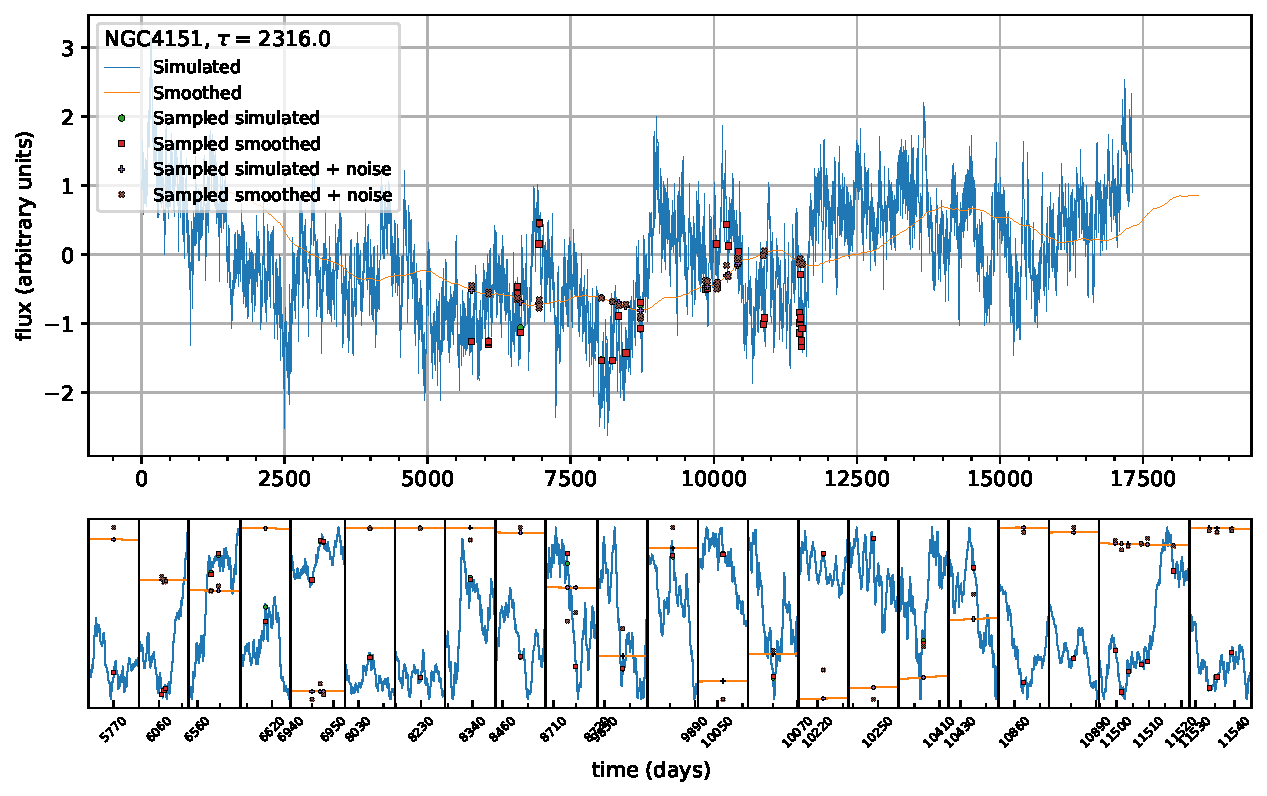
\includegraphics[width=0.49\textwidth]{Figs/Chapter5/NGC4151/sim_LC_tau2316.0_0_matrix.pdf} \\
  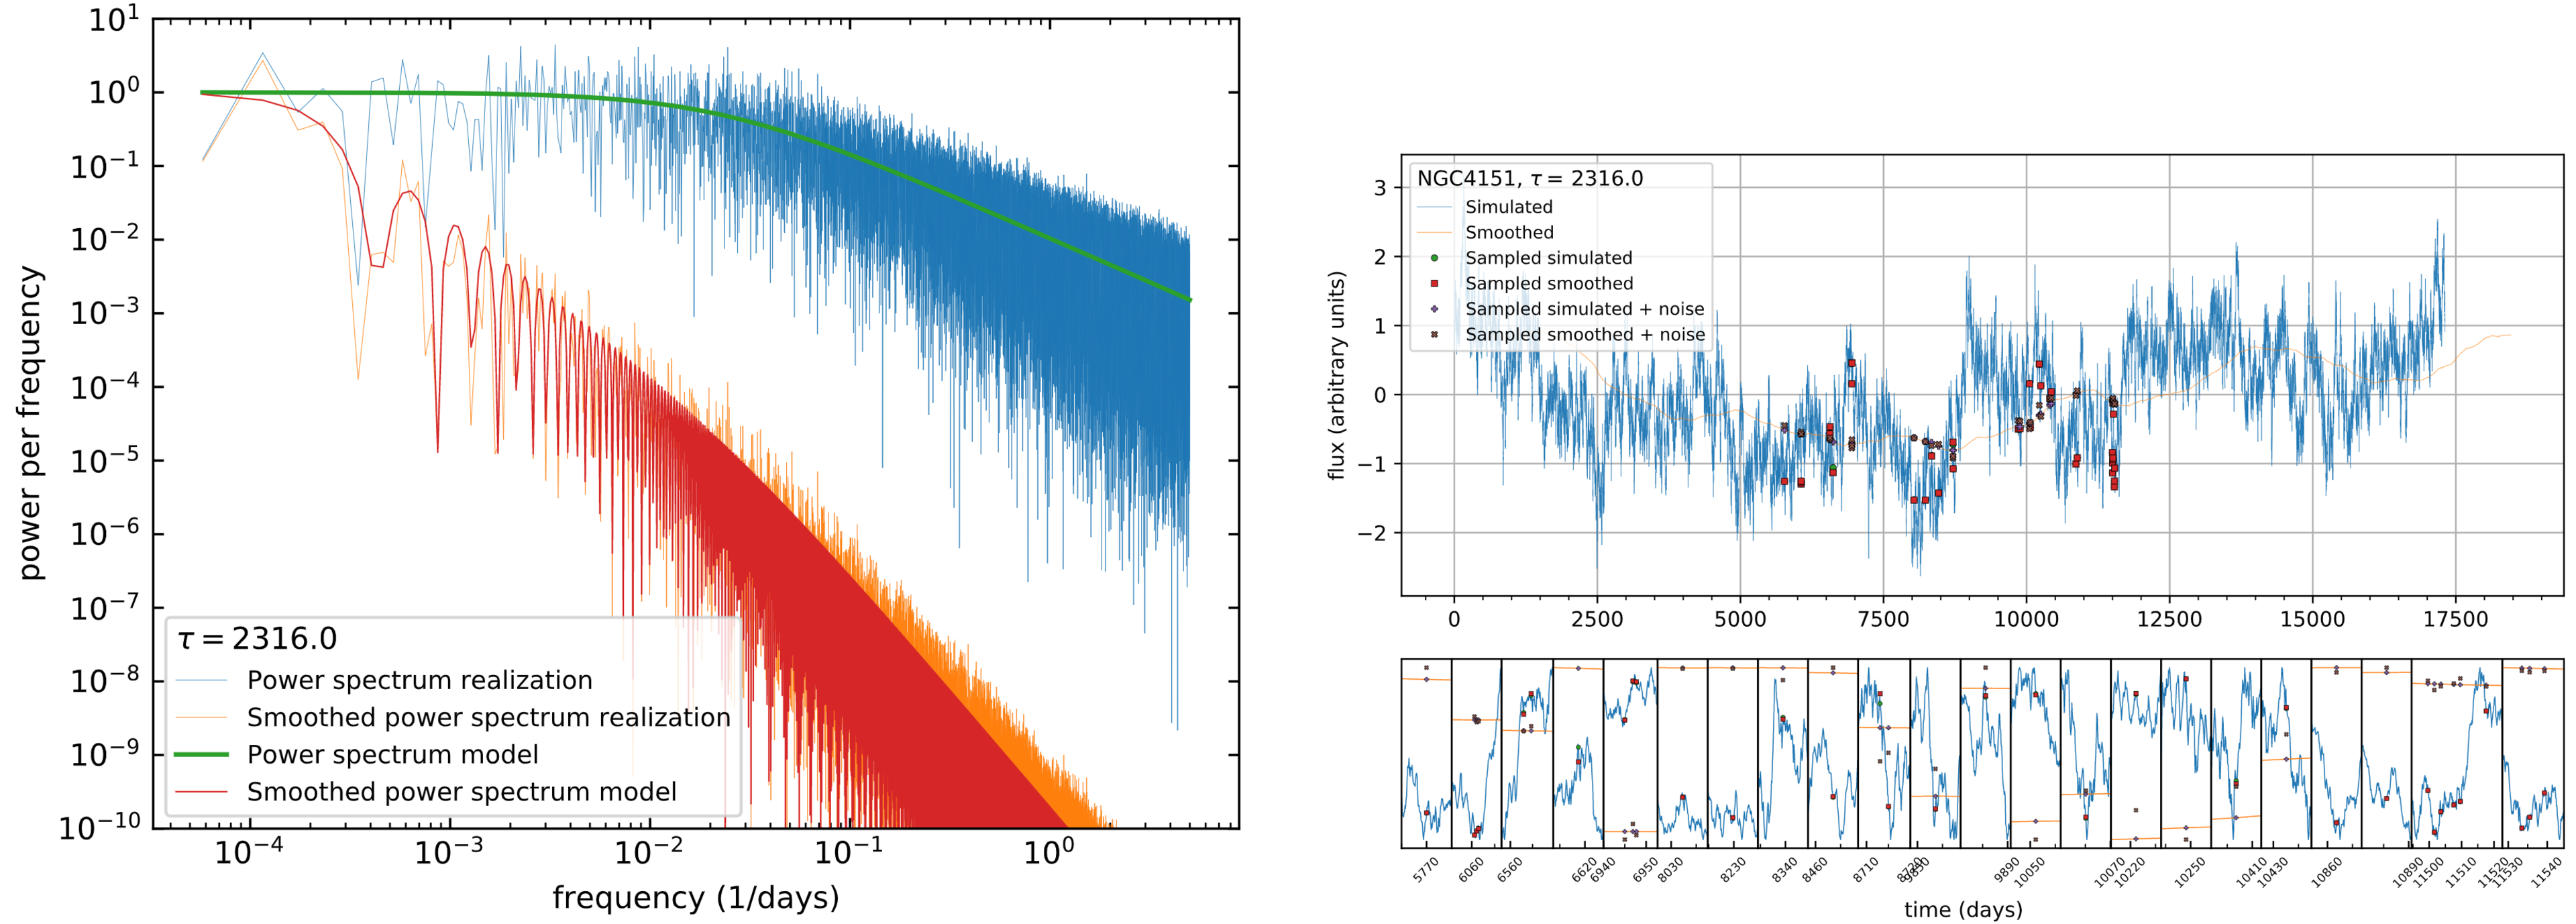
\includegraphics[width=\textwidth]{Figs/Chapter5/NGC4151/Screenshots/NGC4151_tau2316_LC_spectrum.pdf} \\
  \caption{Power spectrum NGC4151}
    \label{fig:power_spectra_1_NGC4151}
  }
\end{center}
\end{figure}

\begin{figure}
\begin{center}
    {
  %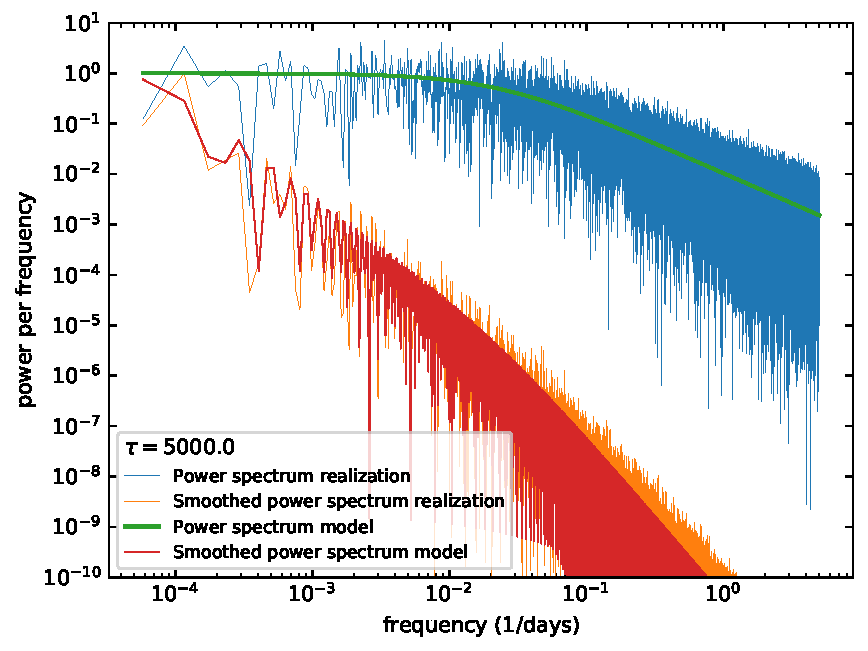
\includegraphics[width=0.49\textwidth]{Figs/Chapter5/NGC4151/power_spectrum_tau5000.0.pdf} \hfill 
  %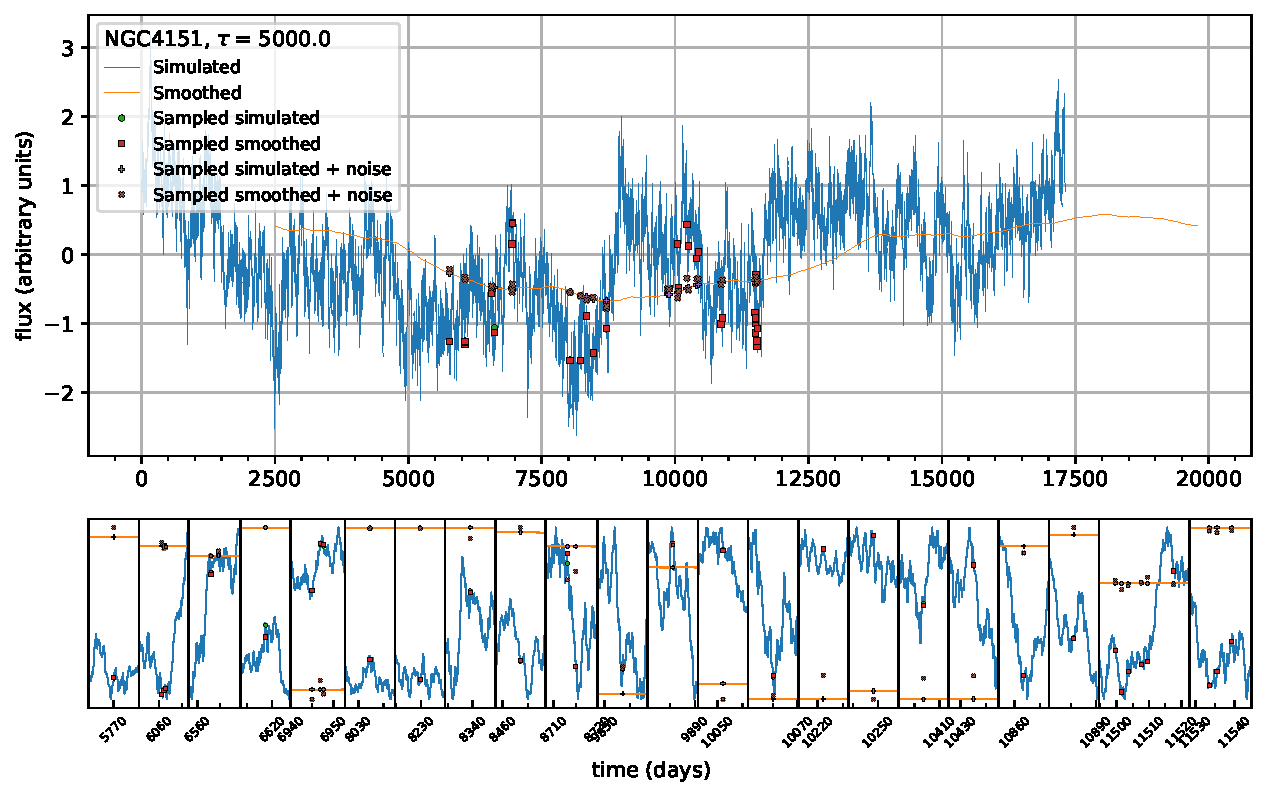
\includegraphics[width=0.49\textwidth]{Figs/Chapter5/NGC4151/sim_LC_tau5000.0_0_matrix.pdf} \\
  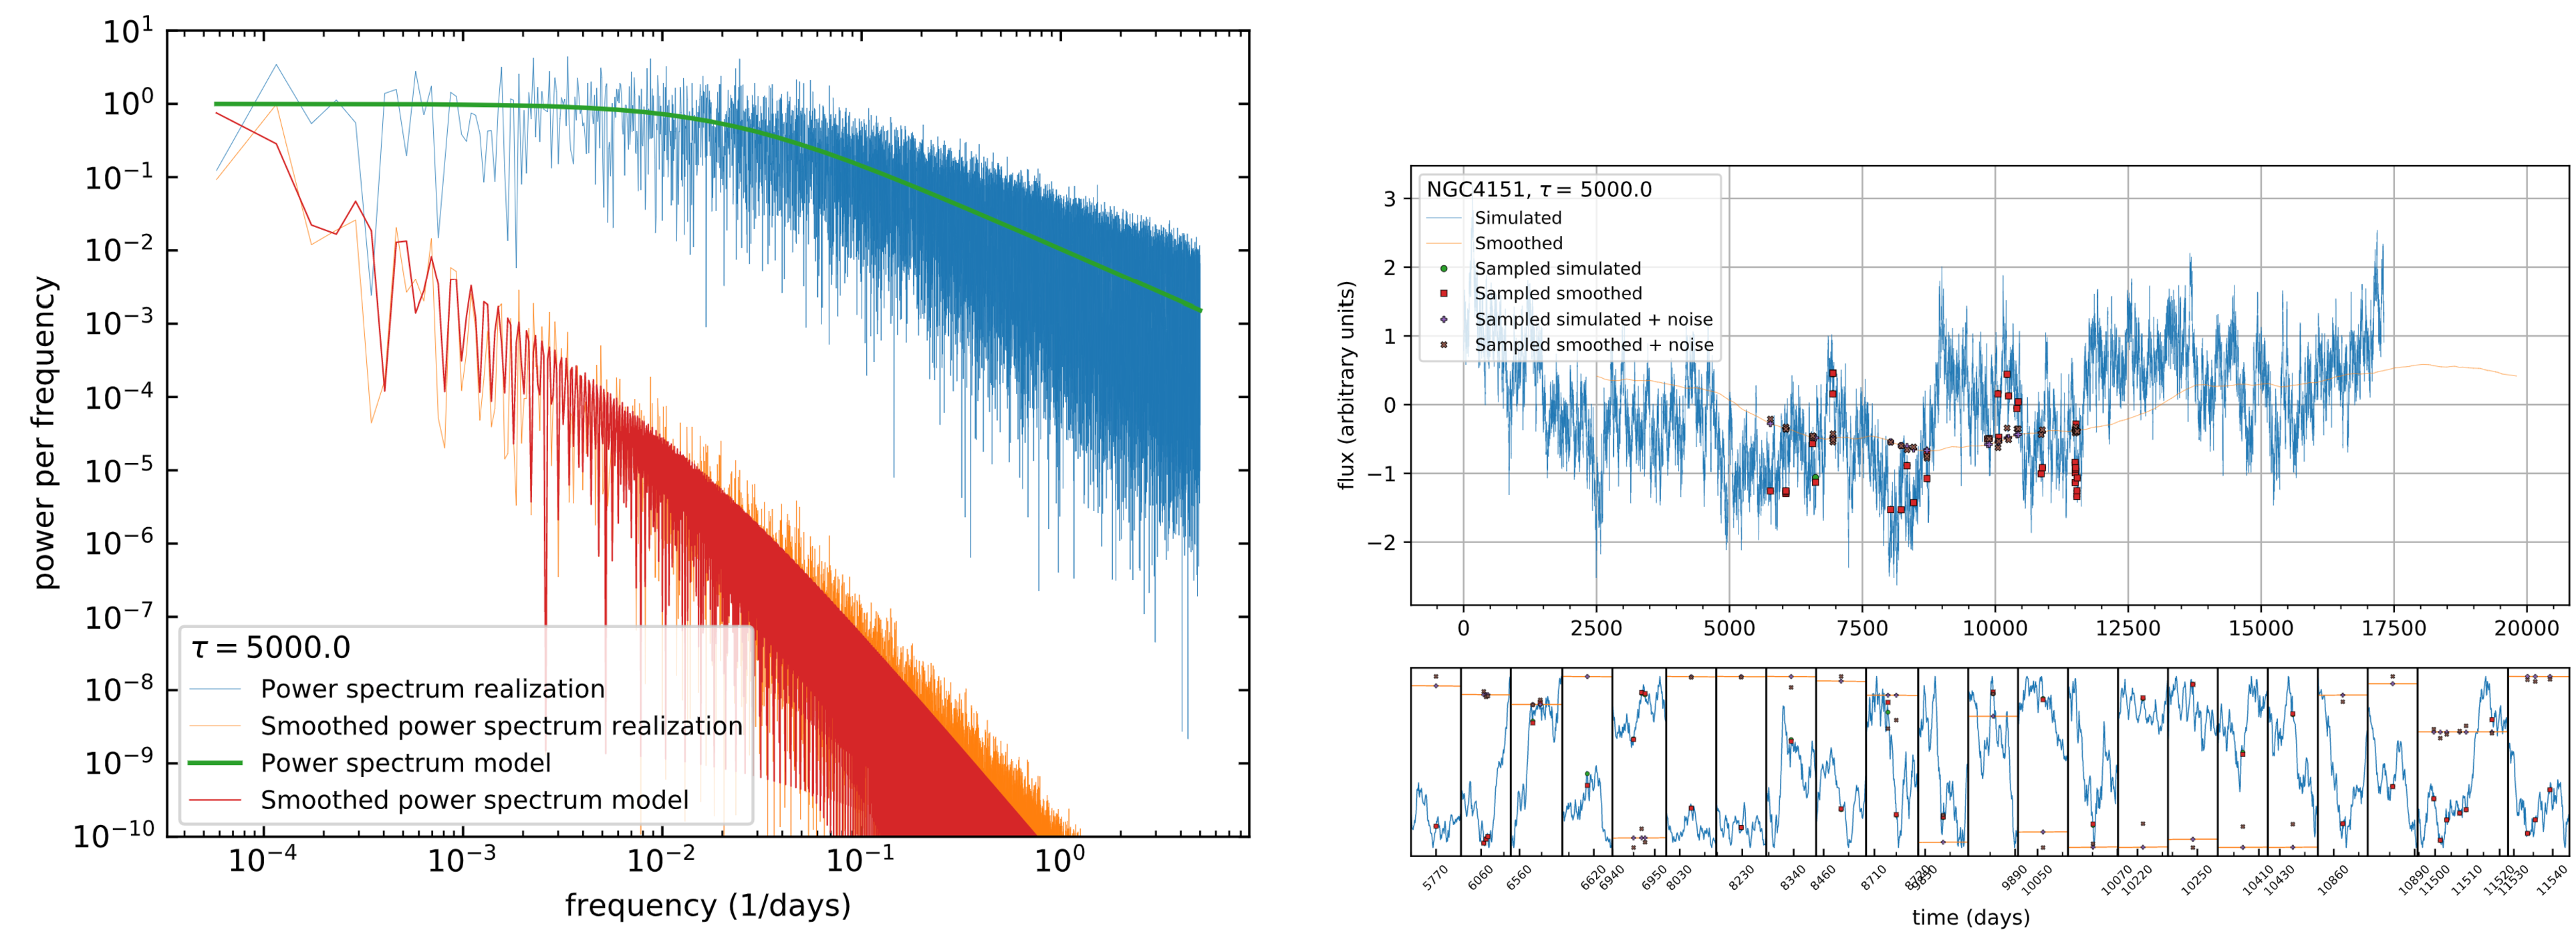
\includegraphics[width=\textwidth]{Figs/Chapter5/NGC4151/Screenshots/NGC4151_tau5000_LC_spectrum.pdf} \\
  %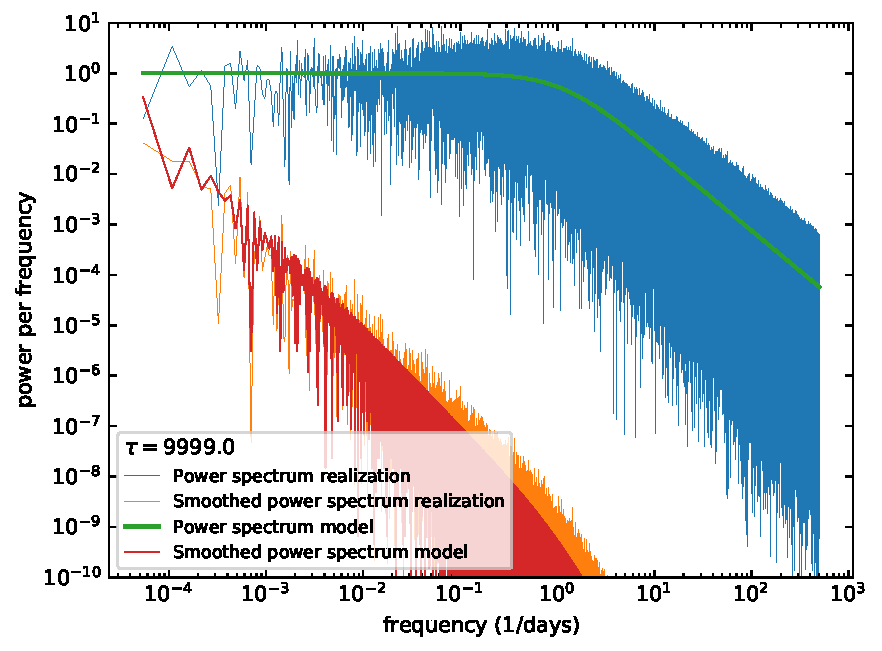
\includegraphics[width=0.49\textwidth]{Figs/Chapter5/NGC4151/power_spectrum_tau9999.0.pdf} \hfill 
  %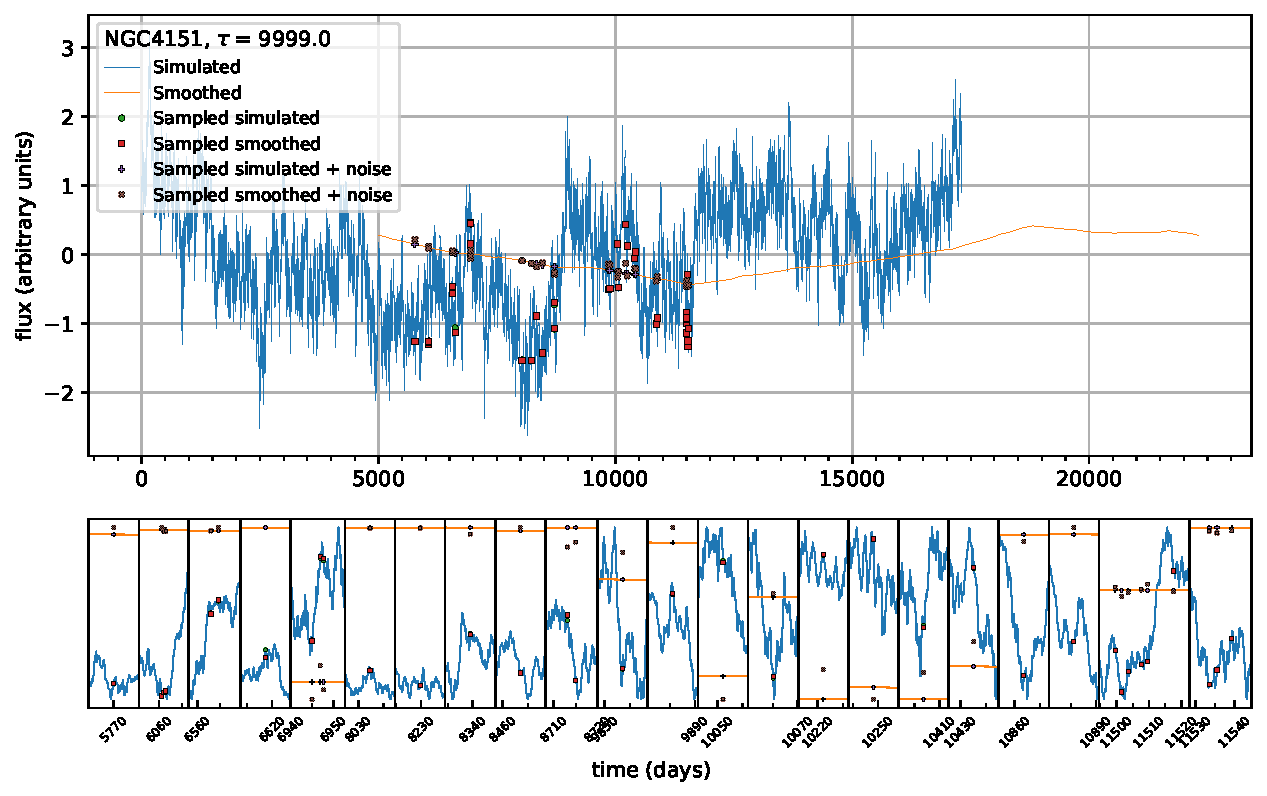
\includegraphics[width=0.49\textwidth]{Figs/Chapter5/NGC4151/sim_LC_tau9999.0_0_matrix.pdf} \\
  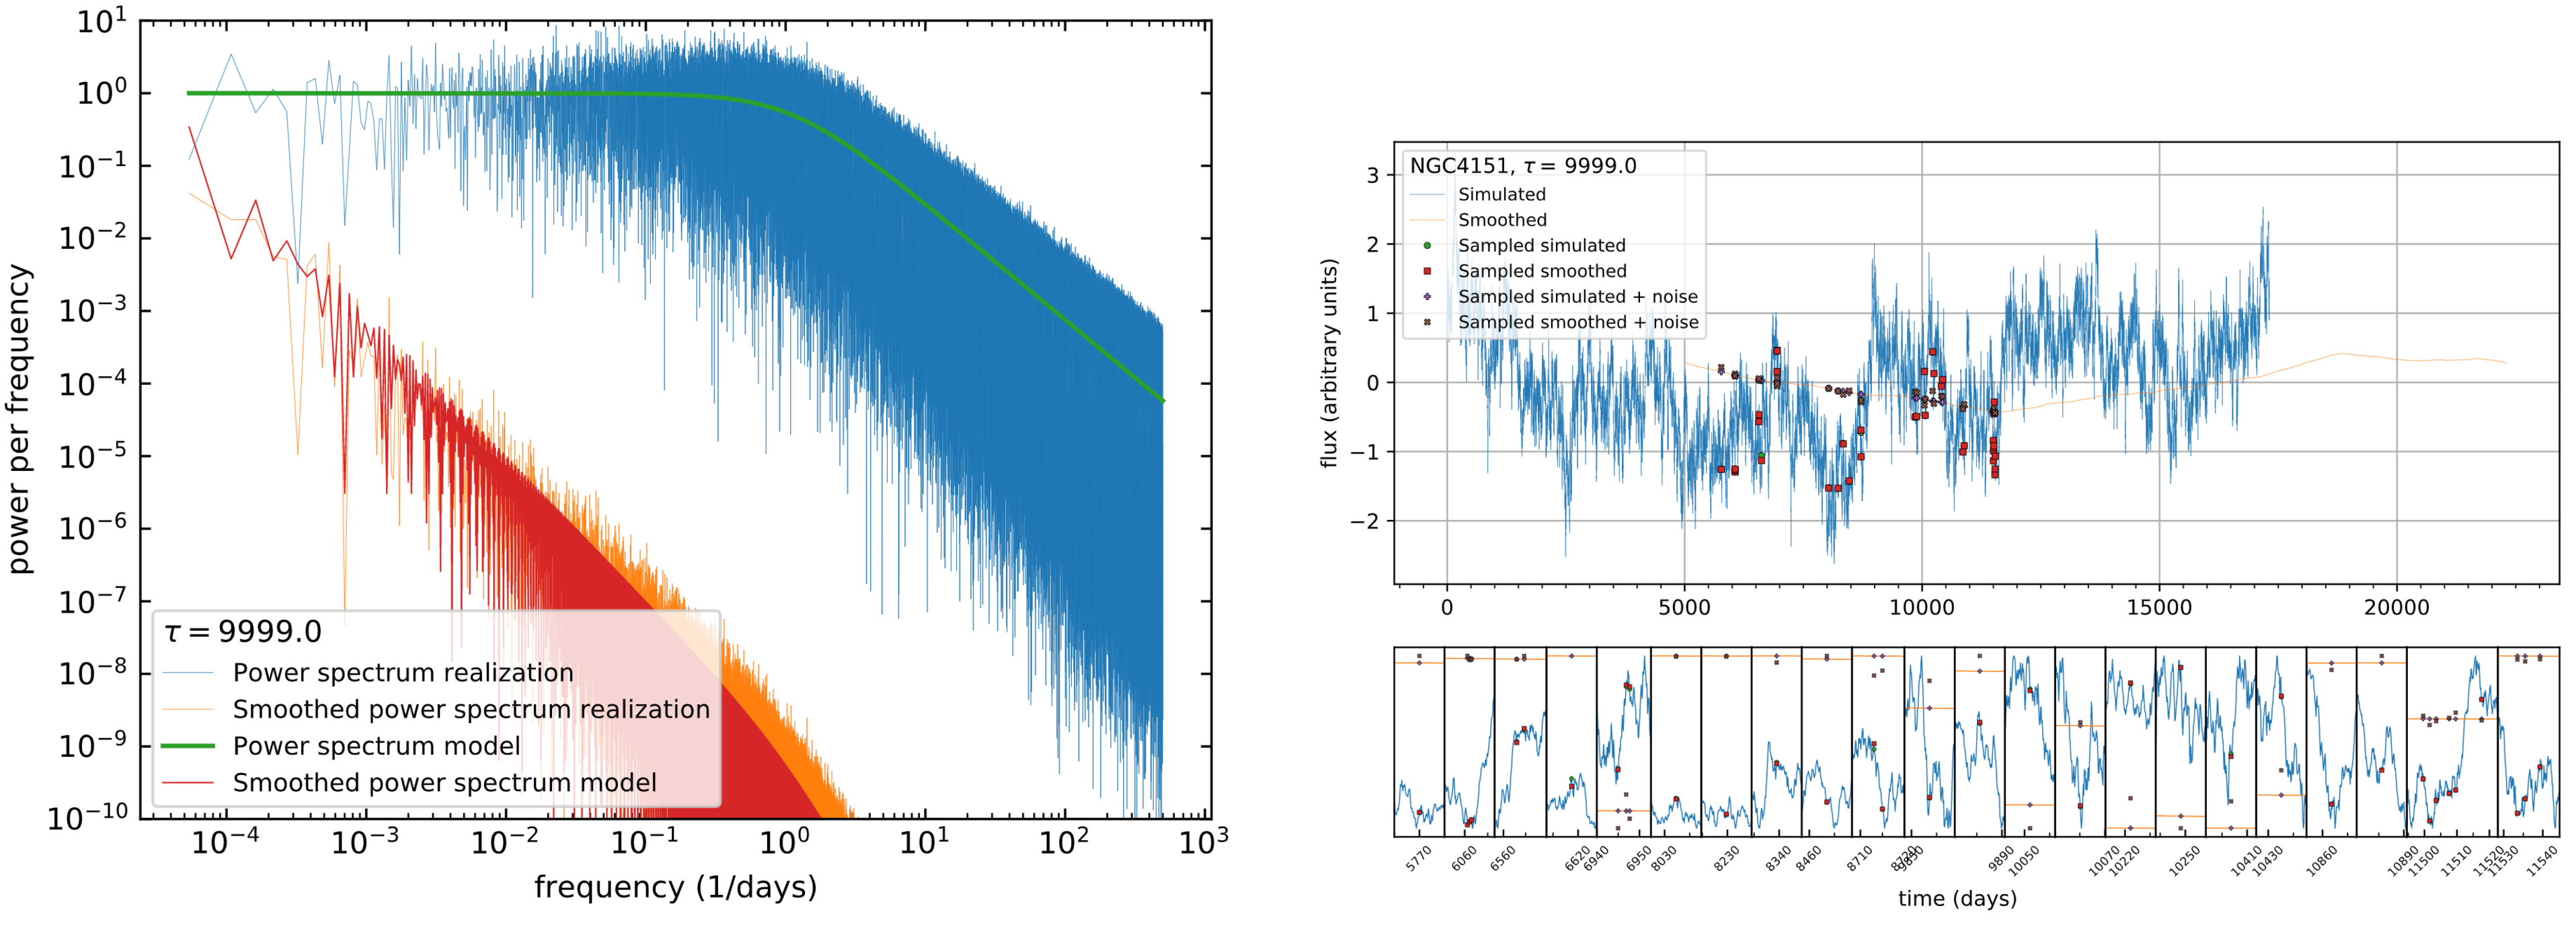
\includegraphics[width=\textwidth]{Figs/Chapter5/NGC4151/Screenshots/NGC4151_tau9999_LC_spectrum.pdf} \\
  \caption{Power spectrum NGC4151}
    \label{fig:power_spectra_2_NGC4151}
  }
\end{center}
\end{figure}

For each source we consider its spectral parameters and in particular we choose a sampling time-scale $dt$ based on its bending time-scale as $dt=10^{{\rm floor}(\log_{10}(T_b/100)}$, i.e. the sampling resolution is at least a 100th of the $T_b$ scale and is an entire number in the representation $\log(dt)$. This choice results in values $-4\le\log(dt)\le-1$. We resampled the simulated light curves according to the observed epochs and added Gaussian noise to each simulated data-point with a standard deviation scaled based on the error of the observation at that epoch, in order to reproduce the additional variance of the data. Finally, we computed the ratio of the variances ($\xi_{\rm r,sim}=\sigma^2_{\rm Fe, sim}/\sigma^2_{\rm c,sim}$). As expected, this ratio decreases as the light crossing time of the reflector increases. We ran sets of 50 simulations and recorded the mean and root-mean-square deviations (rms) of $\xi_{\rm r,sim}$ for a range of values of the light crossing time. We implemented the following statistic to find the $\tau$ values which correspond to our estimated reprocessor size and its upper and lower limits:
\begin{equation}
    {\rm X}(\tau)=\frac{\xi_{\rm data}-<\xi_{\rm sim}>}{(\xi_{\rm sim})_{rms}}
    \label{eq:X_tau}
\end{equation}
 where $\xi_{r,real}$ is the median value of the $\xi_{r}$ distribution. %We solved the equation for $X=0,-1,1$, which correspond to the $\tau$ best fitting value, the upper limit of $\tau$ at $1\sigma$, and lower limit of $\tau$ at $1\sigma$, respectively.  
 
 Examples of the power spectra used to simulate light curves are reported in the left panels of Figs.~\ref{fig:power_spectra_1_NGC3783} and \ref{fig:power_spectra_2_NGC3783} for NGC 3783 and Figs.~\ref{fig:power_spectra_1_NGC4151} and ~\ref{fig:power_spectra_2_NGC4151} for NGC 4151, for both the continuum and \kalfa{} ("smoothed"). These two galaxies were chosen as an example of very different $\nu_b$ frequencies and because we were able to find all three $\tau$ values corresponding to $X=0,1,-1$. In the model power spectrum (green line) we can see a decrease in power after the break frequency, which is $\nu_b=1.1 \,{\rm days}^{-1}$ for NGC 3783 and $\nu_b=0.022\,{\rm days}^{-1}$ for NGC 4151. We also see a decrease in the smoothed power spectrum (red line) at frequencies higher that $1/\tau$, where $\tau$ is shown in the legend title of each figure and is shown in increasing order.
 
    In the right panels of the aforementioned Figures we show the light curves associated with the power spectra on the left, and we also show the resampled data points from the light curves. The blue light curve corresponds to the realization of the power spectrum in blue as well in the left panel, and the orange light curve is the smoothed curve which corresponds to the smoothed power spectrum realization, in orange as well. It can be seen that a higher $\tau$ corresponds to a higher smoothing in the light curve, as expected, and a non obvious correlation between the two light curves, especially with such poor sampling. This can be better seen in the lower panels on the right, which are a zoom in in correspondence to the observed data points, but especially in Fig.~\ref{fig:Flux-flux_NGC3783} and ~\ref{fig:Flux-flux_NGC4151}, which show flux-flux plots for some $\tau$ values. 
 
The $\tau*$ values that return $X=0,1,-1$ correspond to the reprocessor size in light days and its upper and lower limits at $\pm1\sigma$, respectively. In order to constrain the size of the reprocessor, we first explore a range of $\tau$ values between 1-10,000 days, and then numerically look for the roots $X=0,1,-1$ using Newton's method. The resulting $X(\tau)$ relations explored for each source are shown in Appendix~\ref{appendix_lightcurves} while the reprocessor sizes thus determined are discussed in Section~\ref{sec:lc_results}.

\section{Correlation between Fe line and continuum flux} \label{sec:lc_results}

A strong, positive correlation between these two fluxes, which is much simpler to assess compared to more complicated lag analyses, should indicate that the reflector lies in close proximity to the source of the X-ray continuum emission. 
Thus we explore potential correlations between the observed 2--10 keV continuum and \kalfa{} %Fe $\rm K\alpha$
line light curves for sources in our sample. As mentioned above, any lag in the \kalfa{} line light curves, which is expected from reprocessing travel time delays, can reduce the apparent correlation between the observed light curves. The degree of loss of correlation is a function of the ratio between the light crossing time of the reprocessor and the characteristic timescales of fluctuations, as well as the geometry of the reprocessor. 

The green data-points and the relative green best fit in Figs.~\ref{fig:Flux-flux_NGC3783},~\ref{fig:Flux-flux_NGC4151} show one realization of the resampled continuum and reprocessed (\kalfa{}) light curves corresponding to our best estimate of the reprocessor size $\tau*$ while in orange and red we show the resampled data points and best fit our our upper and lower limit (one realization). These relations don't necessarily show a correlation between the observed data (shown with brown crosses), and simulated light curves, but this is due to the delay and the sampling of the data, as we've shown in the previous paragraph, and it doesn't imply that they aren't correlated.

To better show this we refer the reader to Figs.~\ref{fig:Flux-flux_all_1},~\ref{fig:Flux-flux_all_2}~\ref{fig:Flux-flux_all_3}~\ref{fig:Flux-flux_all_4},~\ref{fig:Flux-flux_all_5}, where for each source in our sample for which we were able to determine $\tau*$ such that $X(\tau*)=0$, we show all the best fits of the flux-flux relations of the 50 simulated light curves, versus the data and their best fit, performed with weighted least squares assuming errors on the \kalfa{} line only, as the uncertainty on the \kalfa{} line light curve is generally much higher than in the continuum. For each source we show in the bottom left box the Pearson's correlation coefficient and the Spearman's rank of the observed data, and the reduced $\chi^2$ (or $\tilde\chi^2$) of the fit. The Pearson's correlation coefficient is a measure of linear correlation between the two variables, while the Spearman's rank assesses how well the relationship between the two variables can be described using a monotonic function, and both assume a value of 1 for complete correlation/increasing monotonicity, 0 for no correlation and -1 for complete anti-correlation/decreasing monotonicity. The $\tilde\chi^2$ tells us the quality of the description of the linear fit, so a $\tilde\chi^2\approxeq1$ assesses a good description of the data by the fit, $\tilde\chi^2>1$ indicates that the fit has not fully captured the data, $\tilde\chi^2\gg 1$ indicates a poor model fit, and $\tilde\chi^2<1$ indicates that the model is ``over-fitting'' the data: either the model is improperly fitting noise, or the error variance has been overestimated. In most cases we see values ranging from a decent correlation ($\rho >0.5$) and $\tilde\chi^2>1$ to a poor correlation with $0<\rho <0.5$ and $\tilde\chi^2\gg 1$. We also show in the right panels a histogram of the slopes of the linear fits of the simulations versus the slope of the observed data. We can see that in some cases the slope of the data is compatible with the range of the slopes from the simulated light curves.

We show in Table~\ref{tab:taus} the $\tau*$ values of each source sorted by the median $\xi$. As already mentioned in Section~\ref{sec:variability_defs}, per definition in Eq.~\ref{eq:xi}, the $\xi$ will be $\approx 1$ if the reprocessor is nuclear, i.e. very small, and $\xi\gtrsim 0$ if the reprocessor is extended. 
There are also two cases in which the size of the reprocessor cannot be constrained, these are $\xi<0$ when the uncertainty on the data is greater than their variation, and $\xi>1$ if the variance of the \kalfa{} line is greater than that of the continuum. 
The first case, $\xi<0$, occurs when the uncertainty on the data is greater than their variation and this happens to be the case for the \kalfa{} light curve of the affected sources. However, the upper limit on the ratio of excess variance of these sources is still $>0$, therefore it could also be a matter of overestimation of the noise because of the error on the noise (Eq.~\ref{eq:NXS_err}).
In the latter case, $\xi>1$, either the poor sampling of the light cures did not seize the wider variations of the continuum, or the \kalfa{} line may not be reflecting the variations of the continuum and therefore the reprocessor cannot be modeled in our physical description of the AGN as introduced in Sec.~\ref{sec:LC_sims}. A physical example of this situation could be a radio loud source where a cloud reflects towards us the beamed X-ray emission associated with the powerful jets, leading to stronger and/or more rapid variations in the \kalfa{} line than in the continuum.
We see in Table~\ref{tab:taus} that we were not able to constrain the $\tau*$ values when $\xi<0$ and $\xi>1$, mainly because data quality was poor. Instead, in the intermediate cases we were able to place some constraints, especially when both the upper and lower limits of $\xi$ are well constrained in the range (0,1), like in the cases of NGC 2992, NGC 7582, NGC 4388, NGC 1365, NGC 4151, NGC 3783, MRK 1040. When $\xi$ and its lower limit were very low and/or compatible with negative, meaning that the reprocessor is very extended, we were able to determine a lower limit on the size of the reprocessor. On the contrary, when $\xi$ and its upper limit were close to one, meaning that the reprocessor is small, we were able to place an upper limit on the size of the reprocessor. Roughly $\approx$22\% (9/41) lie above 1, although all are consistent with unity (red line in Fig.~\ref{fig:exvars}) to within 2-$\sigma$ uncertainties. In total, more than 50\% have values consistent with unity, implying little damping of the continuum by the reflector (i.e., angle-averaged light-crossing timescales to the reflector comparable to the continuum variability timescales), or alternatively that we are not observing the true continuum fluctuations. Sometimes, when the $\xi$ value was not well constrained and outside of the (0,1) range we were able to determine the size of the reprocessor, but not its $1\sigma$ limits, or maybe we weren't able to determine any constraint. The complete range of $X(\tau)$ determined for each source is shown in Appendix~\ref{appendix_lightcurves}.

We were able to completely constrain the size of the reprocessor, i.e. best value size and $1\sigma$ uncertainties, for a total of 4 sources and at least one of the limits for 13 sources. For the remaining 16 sources we weren't able to constrain the reprocessor size. This is still a remarkable result, given the sparsity of our light curves and the inconsistent quality of the archival data. Furthermore, the physical model we adopt is extremely simple and may not properly describe all of the source. In fact, more realistic distributions could be thicker, clumpier, and have a toroidal or ionization cone-like structure seen at a specific orientation with respect to the line-of-sight, all of which can impact delay times and smoothing.

\begin{longtable}{llrrr}
\label{tab:taus}\\
\toprule
{} & $\xi(50\%)_{16\%}^{84\%}$   & $\tau_{inf}$ & $\tau_{best}$ & $\tau_{sup}$ \\
{} &                           & (light days) &  (light days) & (light days) \\
\midrule
\endhead
\midrule
\multicolumn{5}{r}{{Continued on next page}} \\
\midrule
\endfoot

%\bottomrule
\endlastfoot
3C120                  &      $ -1.3_{-19.}^{6.6} $ &       - &        - &       - \\
CygnusA                &     $ -0.51_{-6.0}^{3.7} $ &       - &        - &       - \\
PictorA                &    $ -0.34_{-3.1}^{0.88} $ &       - &        - &       - \\
1H0707-495             &   $ -0.18_{-0.82}^{0.28} $ &       1 &        - &       - \\
NGC7469                &   $ -0.036_{-1.2}^{0.68} $ &       - &        - &       - \\
NGC2992                &  $ 0.031_{0.019}^{0.040} $ &     377 &     9713 &       - \\
NGC5548                &  $ 0.042_{-0.071}^{0.15} $ &      99 &        - &       - \\
NGC7582                &  $ 0.070_{0.018}^{0.094} $ &     200 &     8548 &       - \\
MRK766                 &    $ 0.11_{-0.35}^{0.43} $ &       - &       18 &       - \\
MRK290                 &      $ 0.13_{-1.7}^{1.4} $ &       - &      231 &       - \\
2MASXJ11315154-1231587 &   $ 0.20_{-0.026}^{0.39} $ &     112 &     3168 &       - \\
NGC4388                &     $ 0.20_{0.13}^{0.26} $ &       2 &     3013 &    6602 \\
NGC1365                &     $ 0.22_{0.19}^{0.25} $ &      45 &     1999 &    4652 \\
NGC4151                &     $ 0.24_{0.22}^{0.25} $ &     726 &     2316 &    5000 \\
NGC3393                &      $ 0.29_{-1.7}^{1.7} $ &       - &        - &       - \\
MRK273                 &     $ 0.43_{-0.90}^{1.0} $ &       - &     1364 &    5703 \\
NGC3783                &     $ 0.45_{0.29}^{0.58} $ &       6 &      271 &    1675 \\
MRK1040                &     $ 0.57_{0.18}^{0.82} $ &       - &       14 &     903 \\
MRK3                   &      $ 0.73_{0.12}^{1.3} $ &       - &        - &       3 \\
MRK509                 &     $ 0.76_{-0.81}^{1.8} $ &       - &       84 &    2418 \\
NGC1275                &     $ 0.82_{0.025}^{1.3} $ &       - &       15 &       - \\
CenA                   &      $ 0.92_{0.66}^{1.1} $ &       - &        - &      51 \\
IC4329A                &      $ 0.99_{0.47}^{1.3} $ &       - &        1 &     385 \\
NGC3516                &      $ 1.0_{-0.68}^{2.0} $ &       - &        - &    1988 \\
CircinusGalaxy         &       $ 1.1_{0.33}^{1.8} $ &       - &        - &       5 \\
NGC4051                &       $ 1.8_{-3.3}^{4.4} $ &       - &        - &       - \\
NGC1068                &        $ 2.3_{1.4}^{2.8} $ &       - &        - &       - \\
MCG-6-30-15            &        $ 3.0_{1.5}^{4.2} $ &       - &        - &       - \\
MRK1210                &       $ 3.4_{0.90}^{6.1} $ &       - &        - &       - \\
4C+29.30               &       $ 3.8_{-27.}^{40.} $ &       - &        - &       - \\
MR2251-178             &        $ 5.3_{2.0}^{7.9} $ &       - &        - &       - \\
4C+74.26               &        $ 7.7_{2.1}^{11.} $ &       - &        - &       - \\
3C273                  &       $ 18._{-17.}^{36.} $ &       - &        - &       - \\
\hline
\caption{For each galaxy we show the $\tau*$ such that $X(\tau_{inf})=-1$, $X(\tau_{best})=-1$, and $X(\tau_{sup})=-1$. We also report the $\xi$ values previously shown in Table \ref{tab:gals_obs_par}, and we order the Table based on this column for clarity reasons.}\\
\end{longtable}

\begin{figure}
\begin{center}
    {
  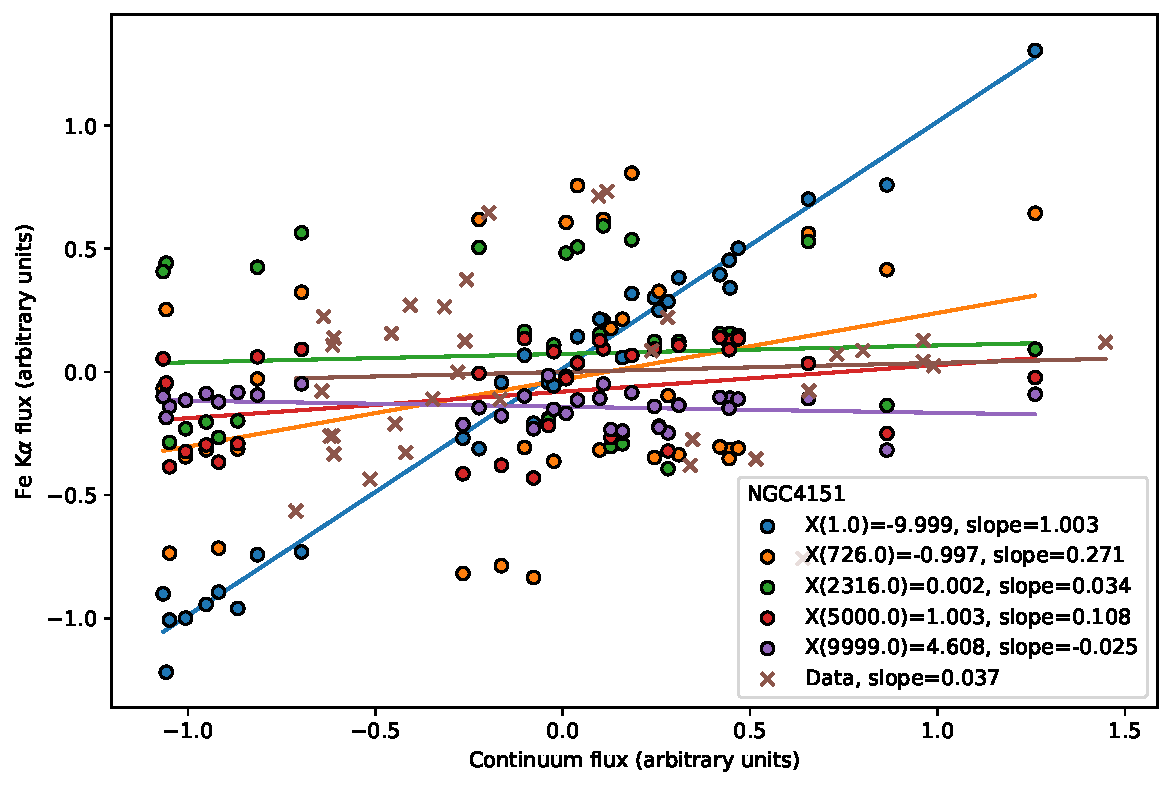
\includegraphics[width=0.7\textwidth]{Figs/Chapter5/NGC4151/Flux_flux_NGC4151.pdf} \hfill 
  \caption{Flux - flux plot NGC4151}
    \label{fig:Flux-flux_NGC4151}
  }
\end{center}
\end{figure}

\begin{figure}
\begin{center}
    {
 % \includegraphics[width=0.49\textwidth]{Figs/Chapter5/NGC3783/power_spectrum_tau1.0.pdf}  \hfill
 % 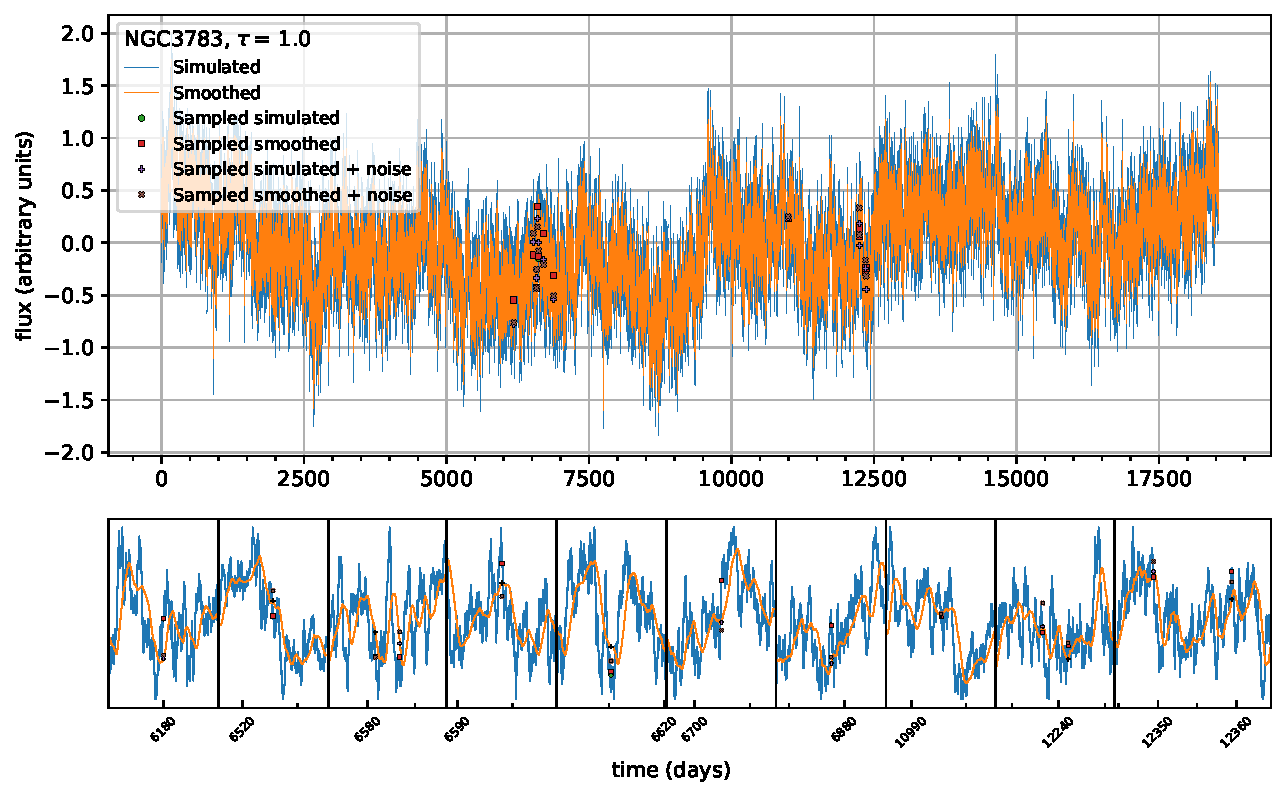
\includegraphics[width=0.49\textwidth]{Figs/Chapter5/NGC3783/sim_LC_tau1.0_0_matrix.pdf} \\
  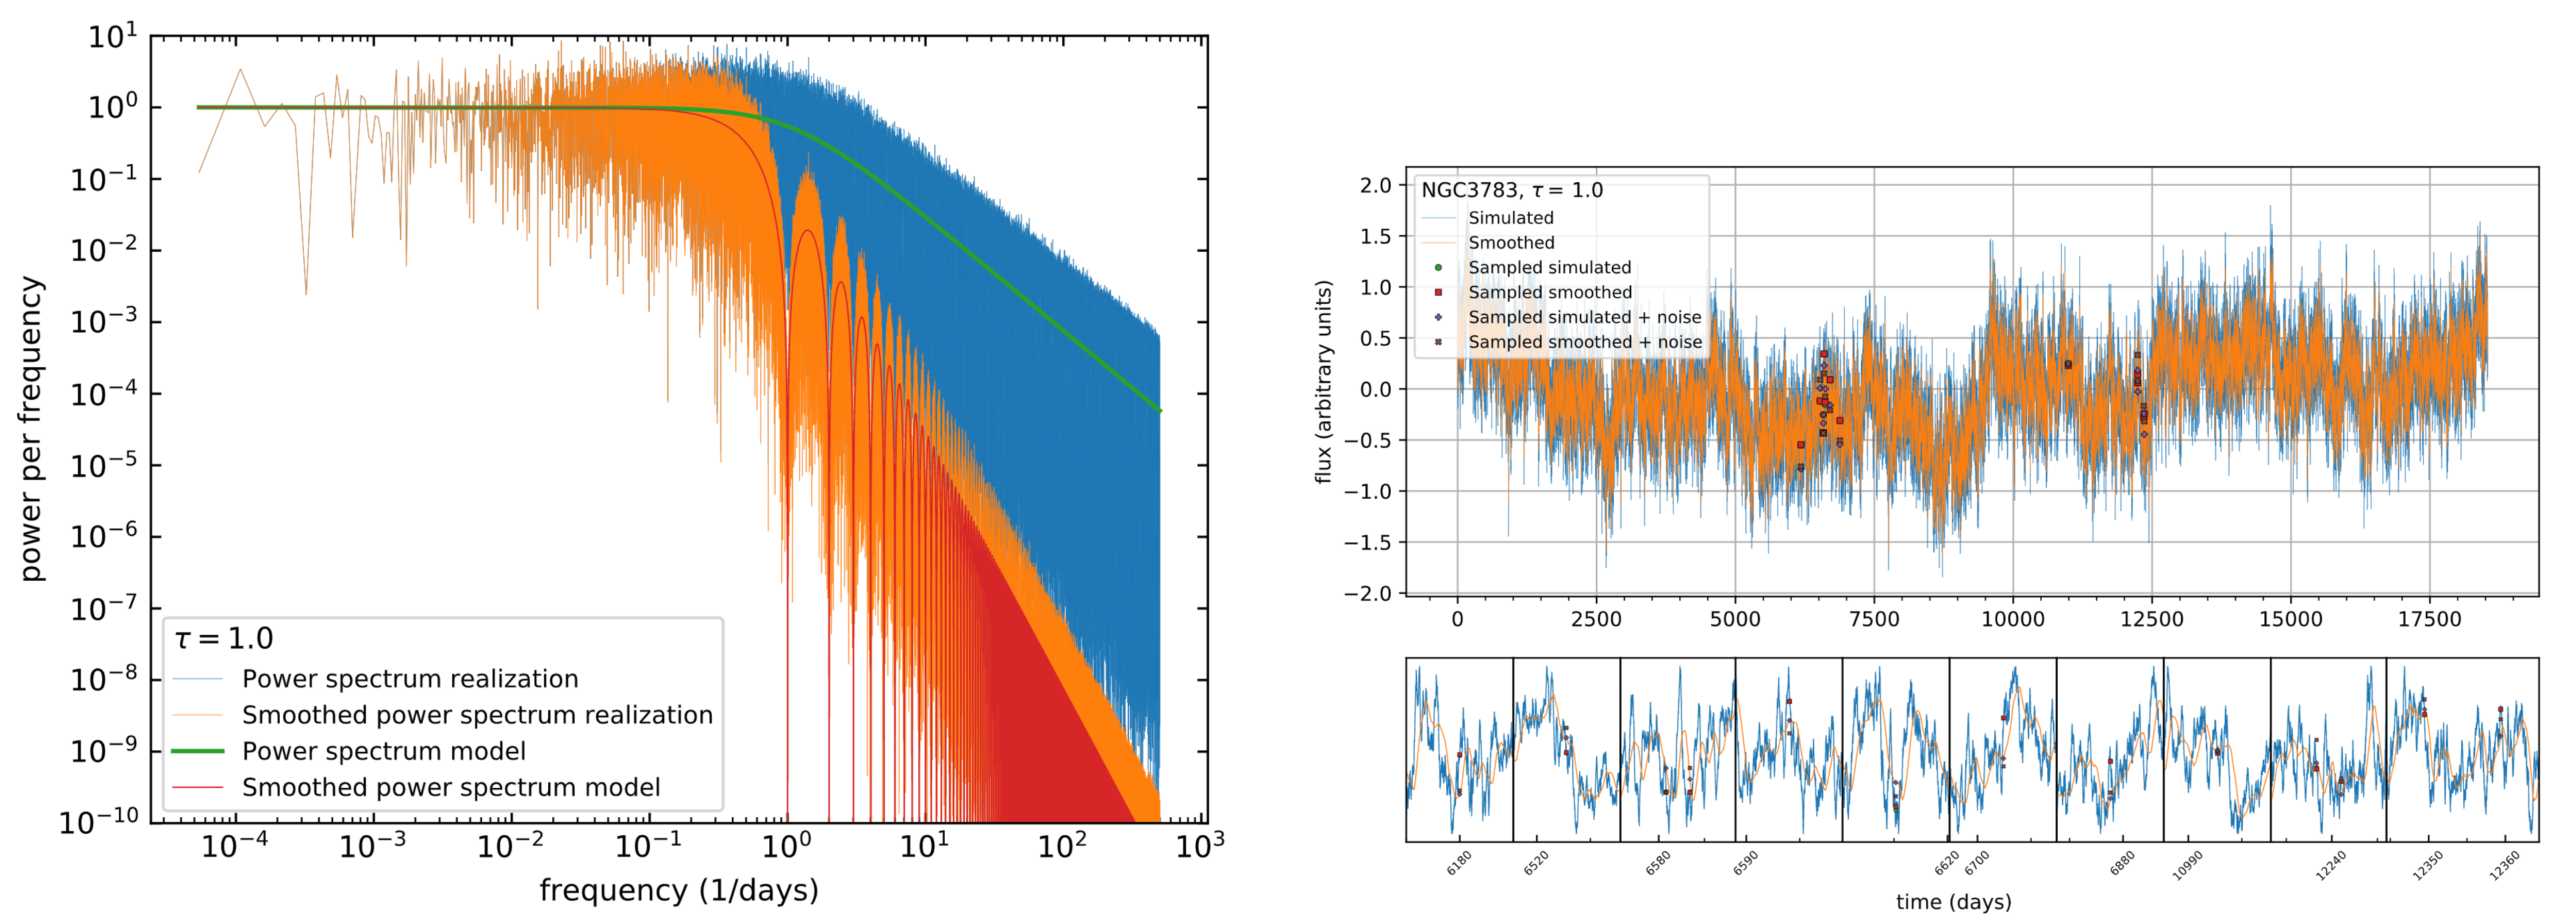
\includegraphics[width=\textwidth]{Figs/Chapter5/NGC3783/Screenshots/NGC3783_tau1_LC_spectrum.pdf} \\
  %\includegraphics[width=0.49\textwidth]{Figs/Chapter5/NGC3783/power_spectrum_tau5.0.pdf}\hfill 
 % 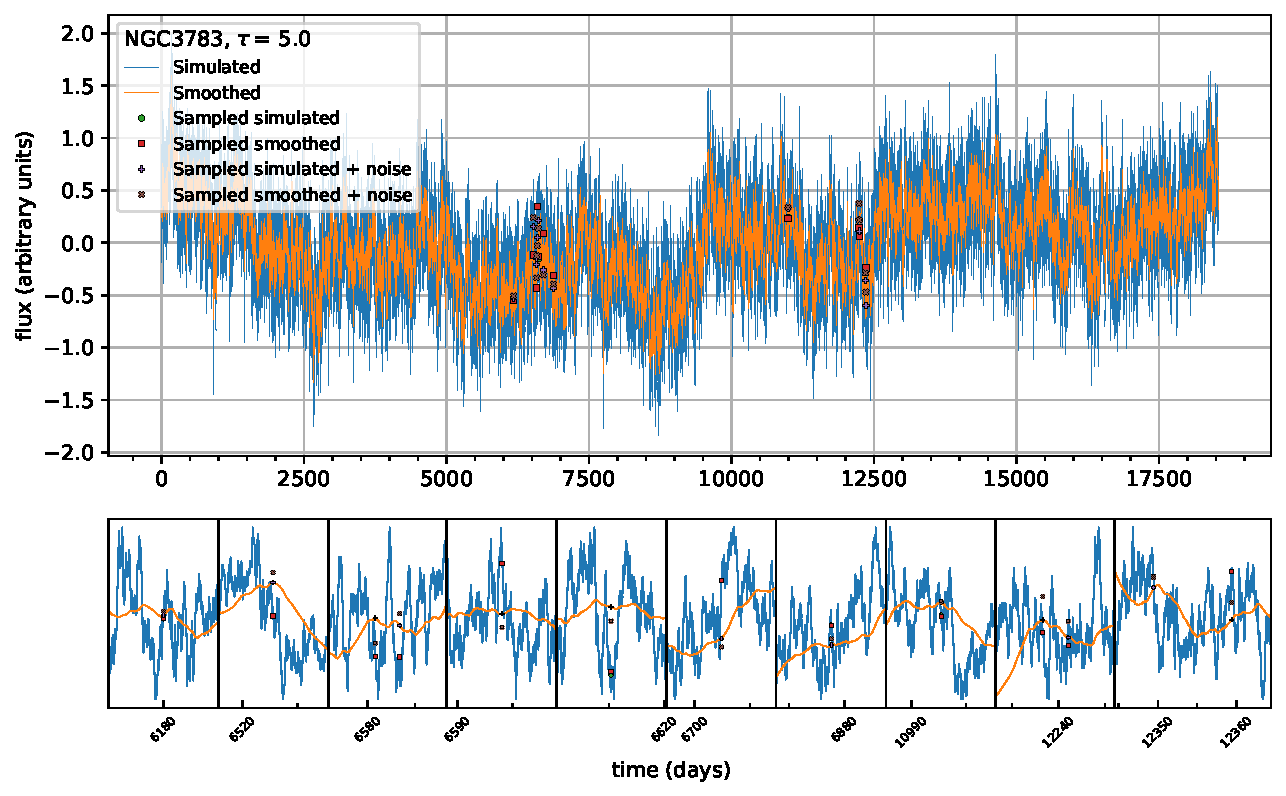
\includegraphics[width=0.49\textwidth]{Figs/Chapter5/NGC3783/sim_LC_tau5.0_0_matrix.pdf} \\
  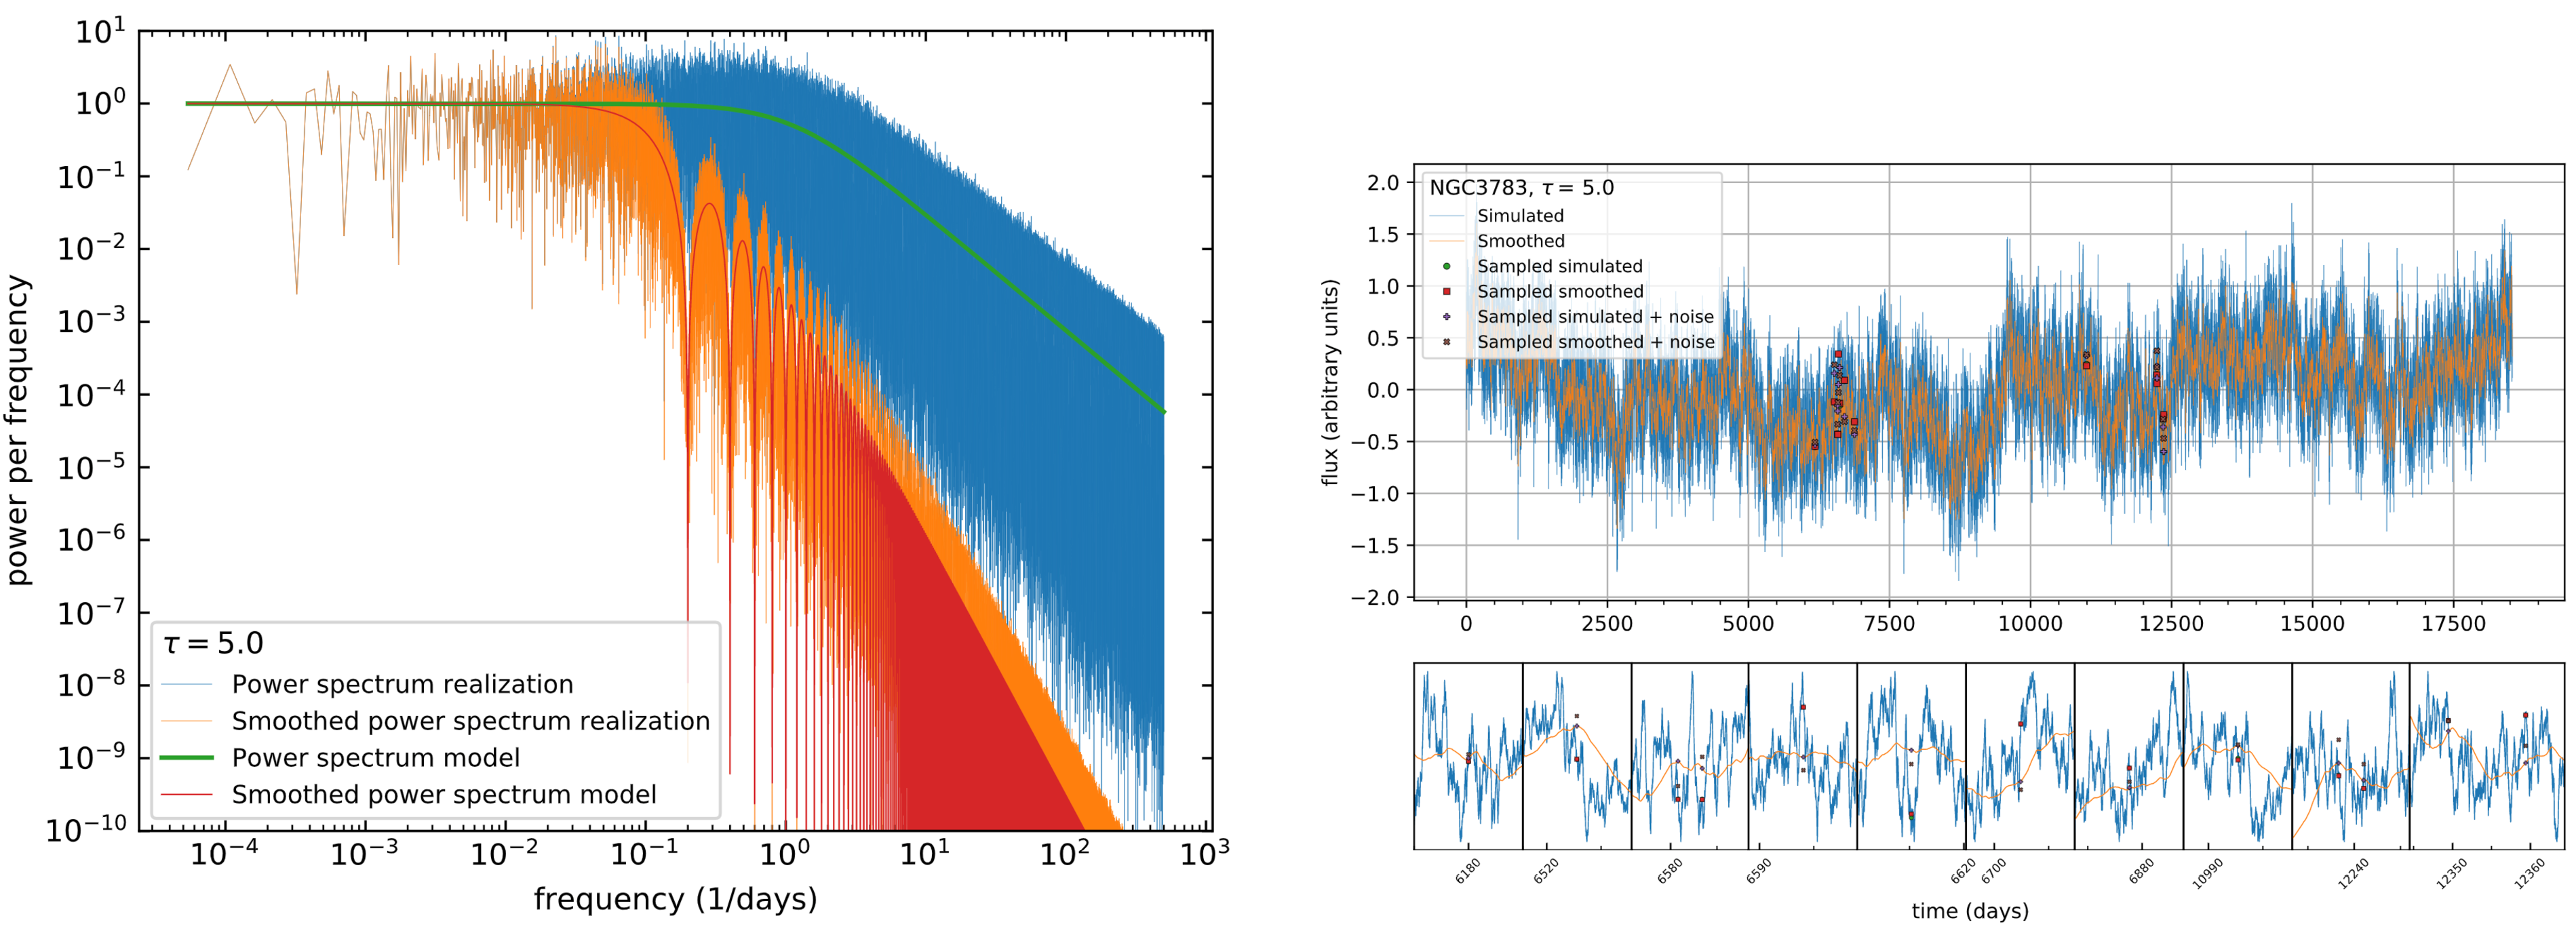
\includegraphics[width=\textwidth]{Figs/Chapter5/NGC3783/Screenshots/NGC3783_tau5_LC_spectrum.pdf} \\
 % 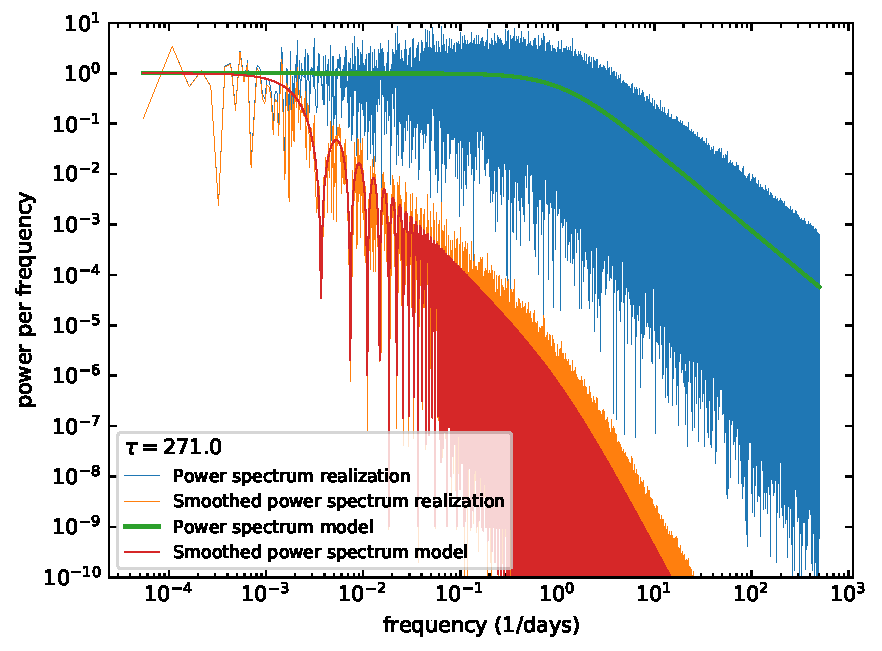
\includegraphics[width=0.49\textwidth]{Figs/Chapter5/NGC3783/power_spectrum_tau271.0.pdf} \hfill 
 % 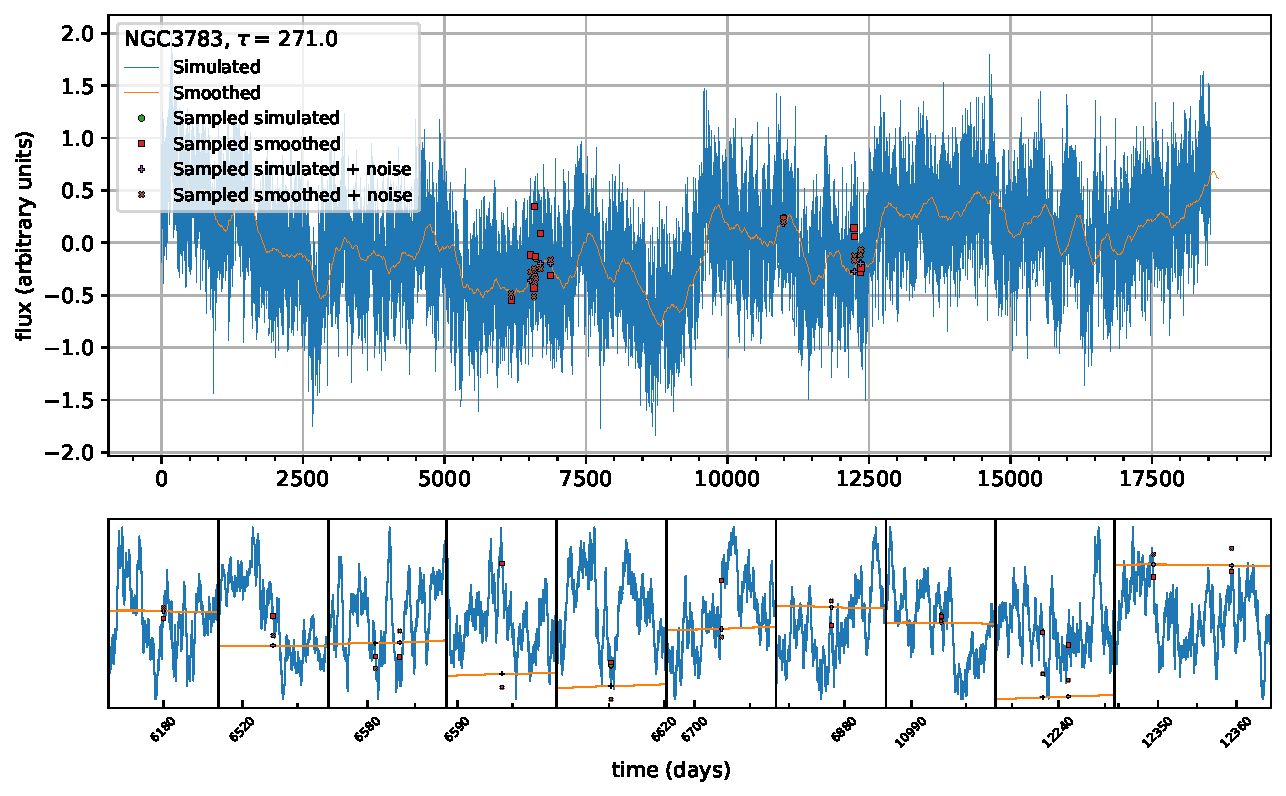
\includegraphics[width=0.49\textwidth]{Figs/Chapter5/NGC3783/sim_LC_tau271.0_0_matrix.pdf} \\
  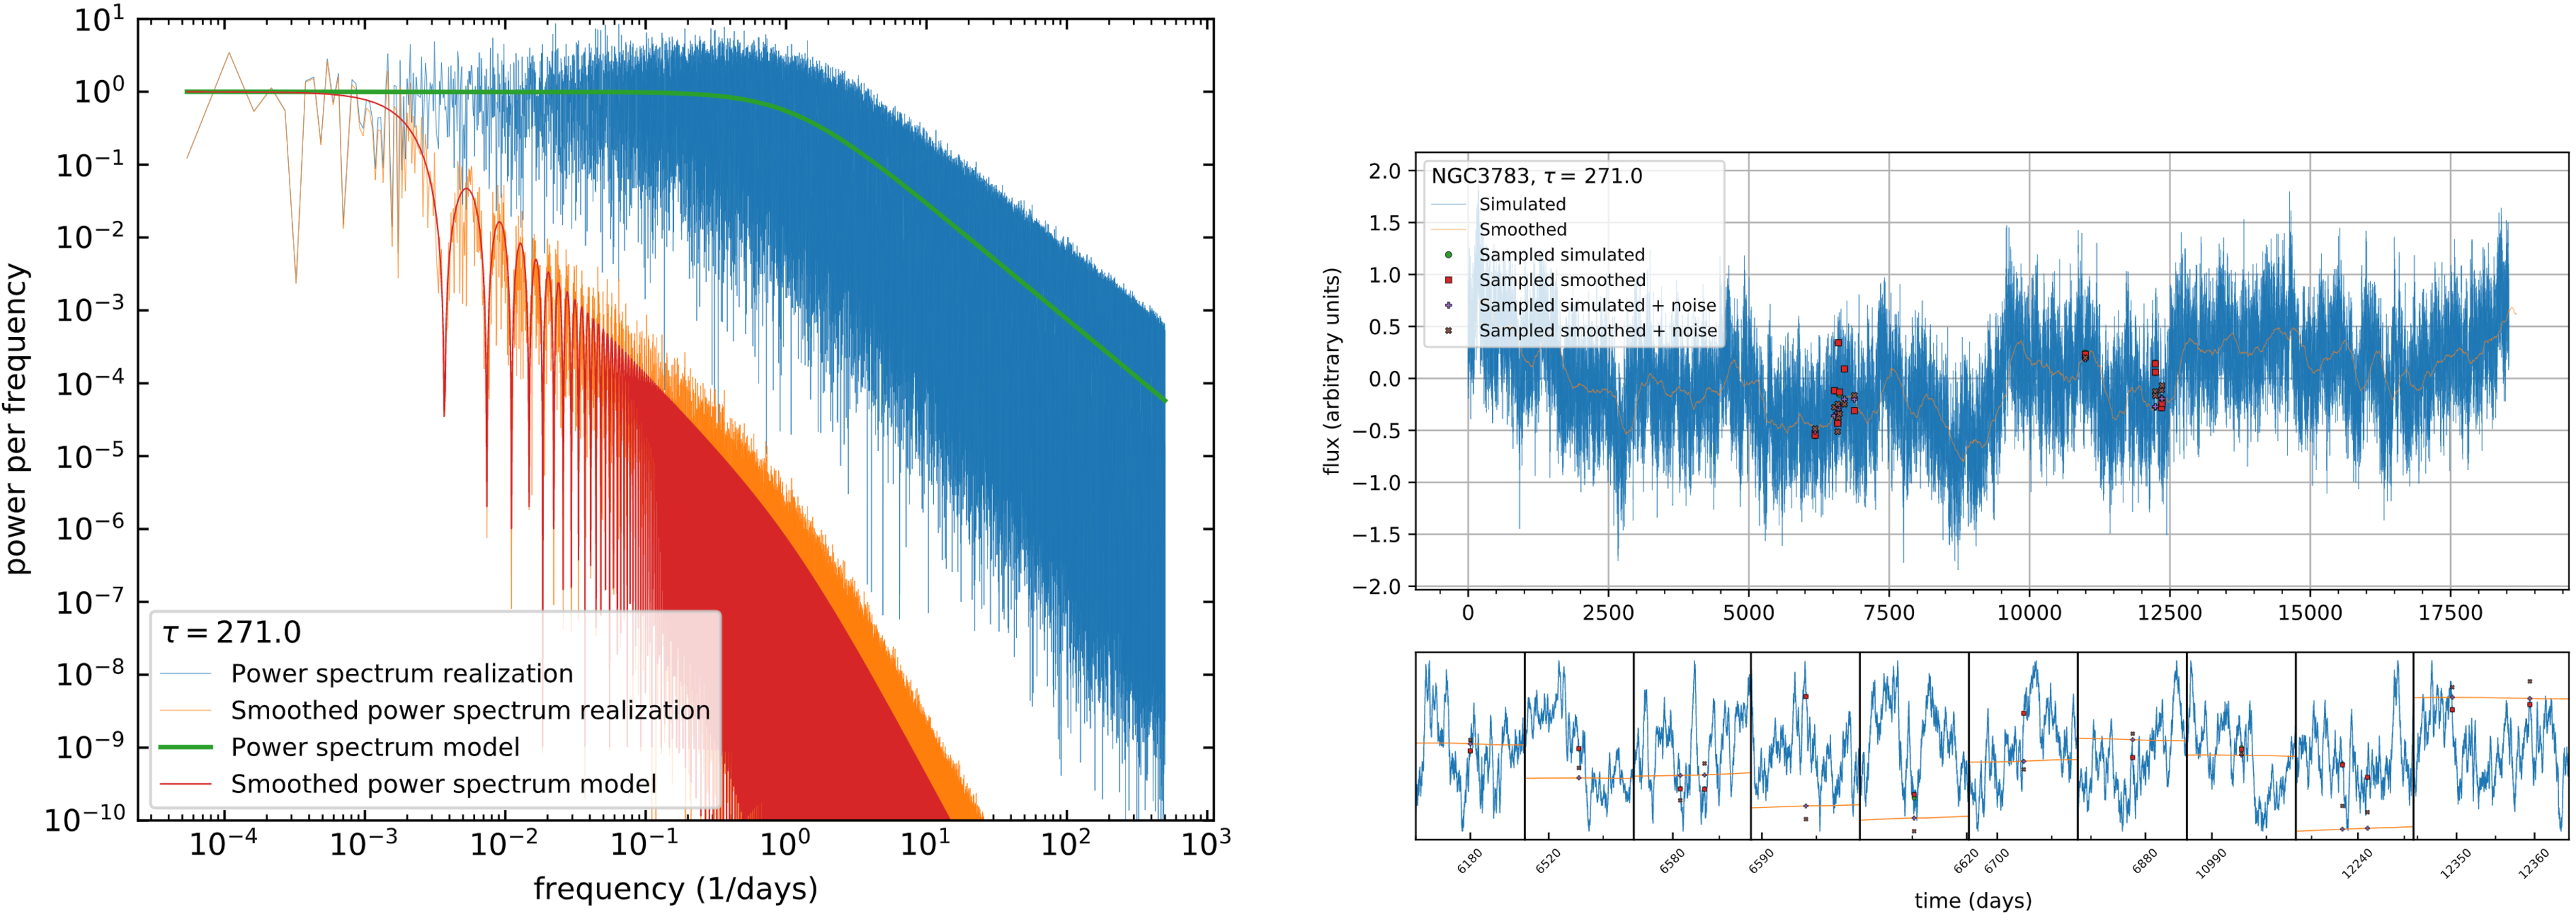
\includegraphics[width=\textwidth]{Figs/Chapter5/NGC3783/Screenshots/NGC3783_tau271_LC_spectrum.pdf} \\
    \label{fig:power_spectra_1_NGC3783}
  }
\end{center}
\end{figure}

\begin{figure}
\begin{center}
    {
 % 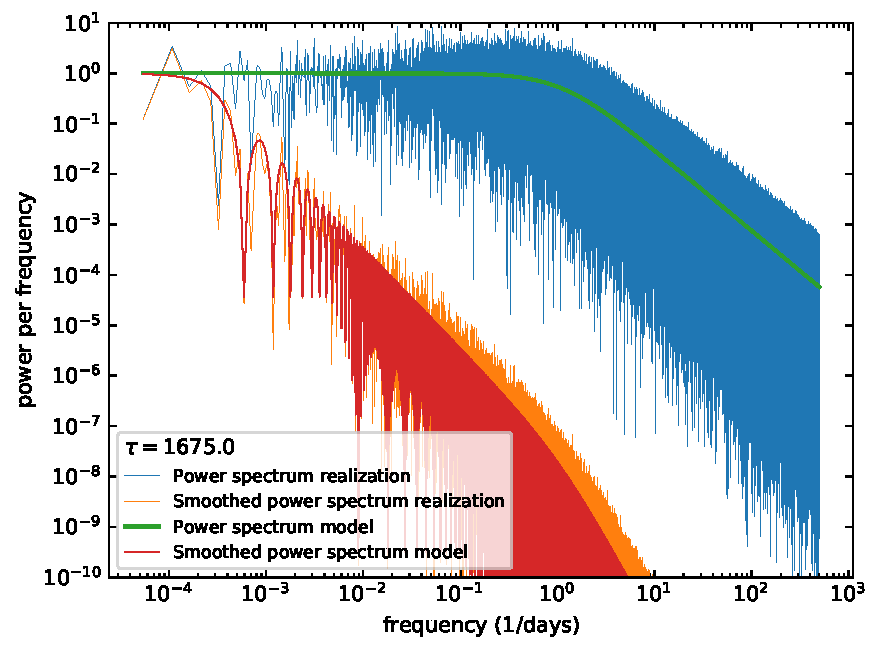
\includegraphics[width=0.49\textwidth]{Figs/Chapter5/NGC3783/power_spectrum_tau1675.0.pdf} \hfill 
 % 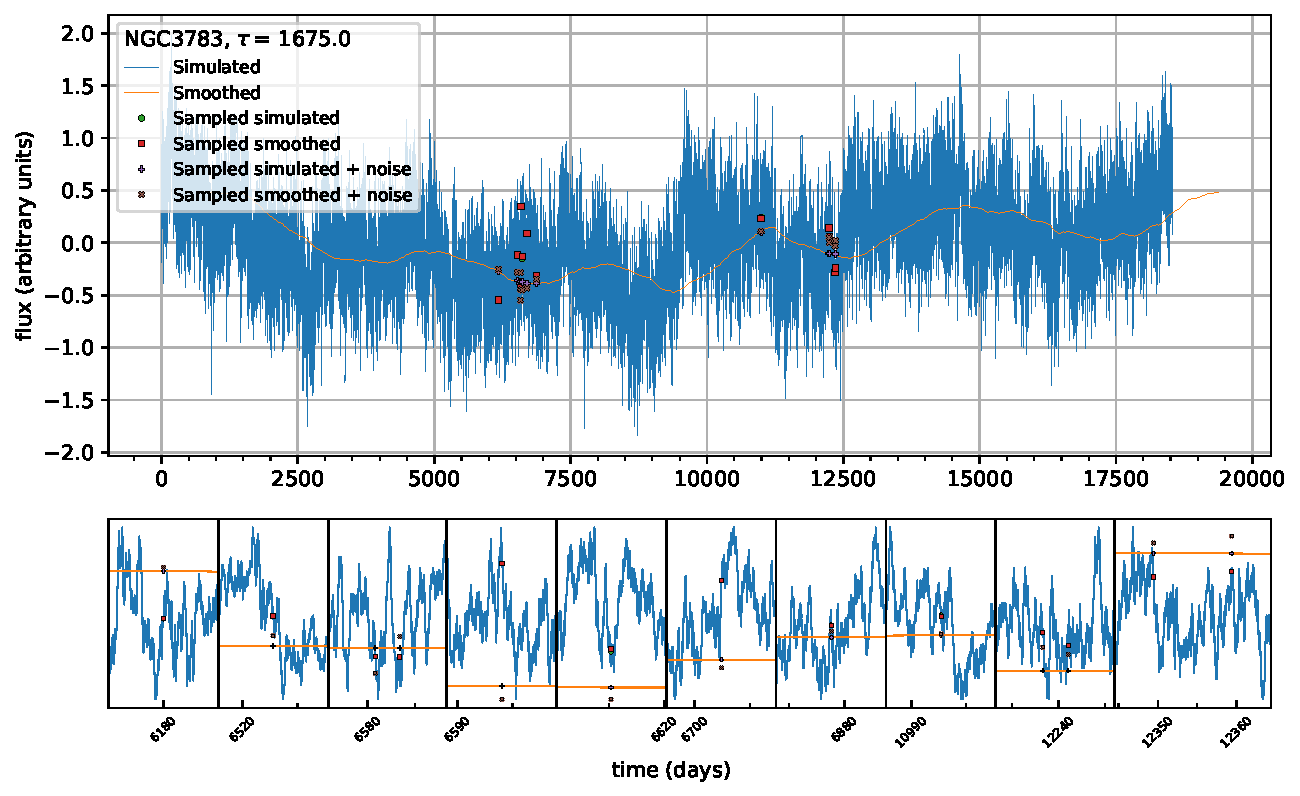
\includegraphics[width=0.49\textwidth]{Figs/Chapter5/NGC3783/sim_LC_tau1675.0_0_matrix.pdf} \\
  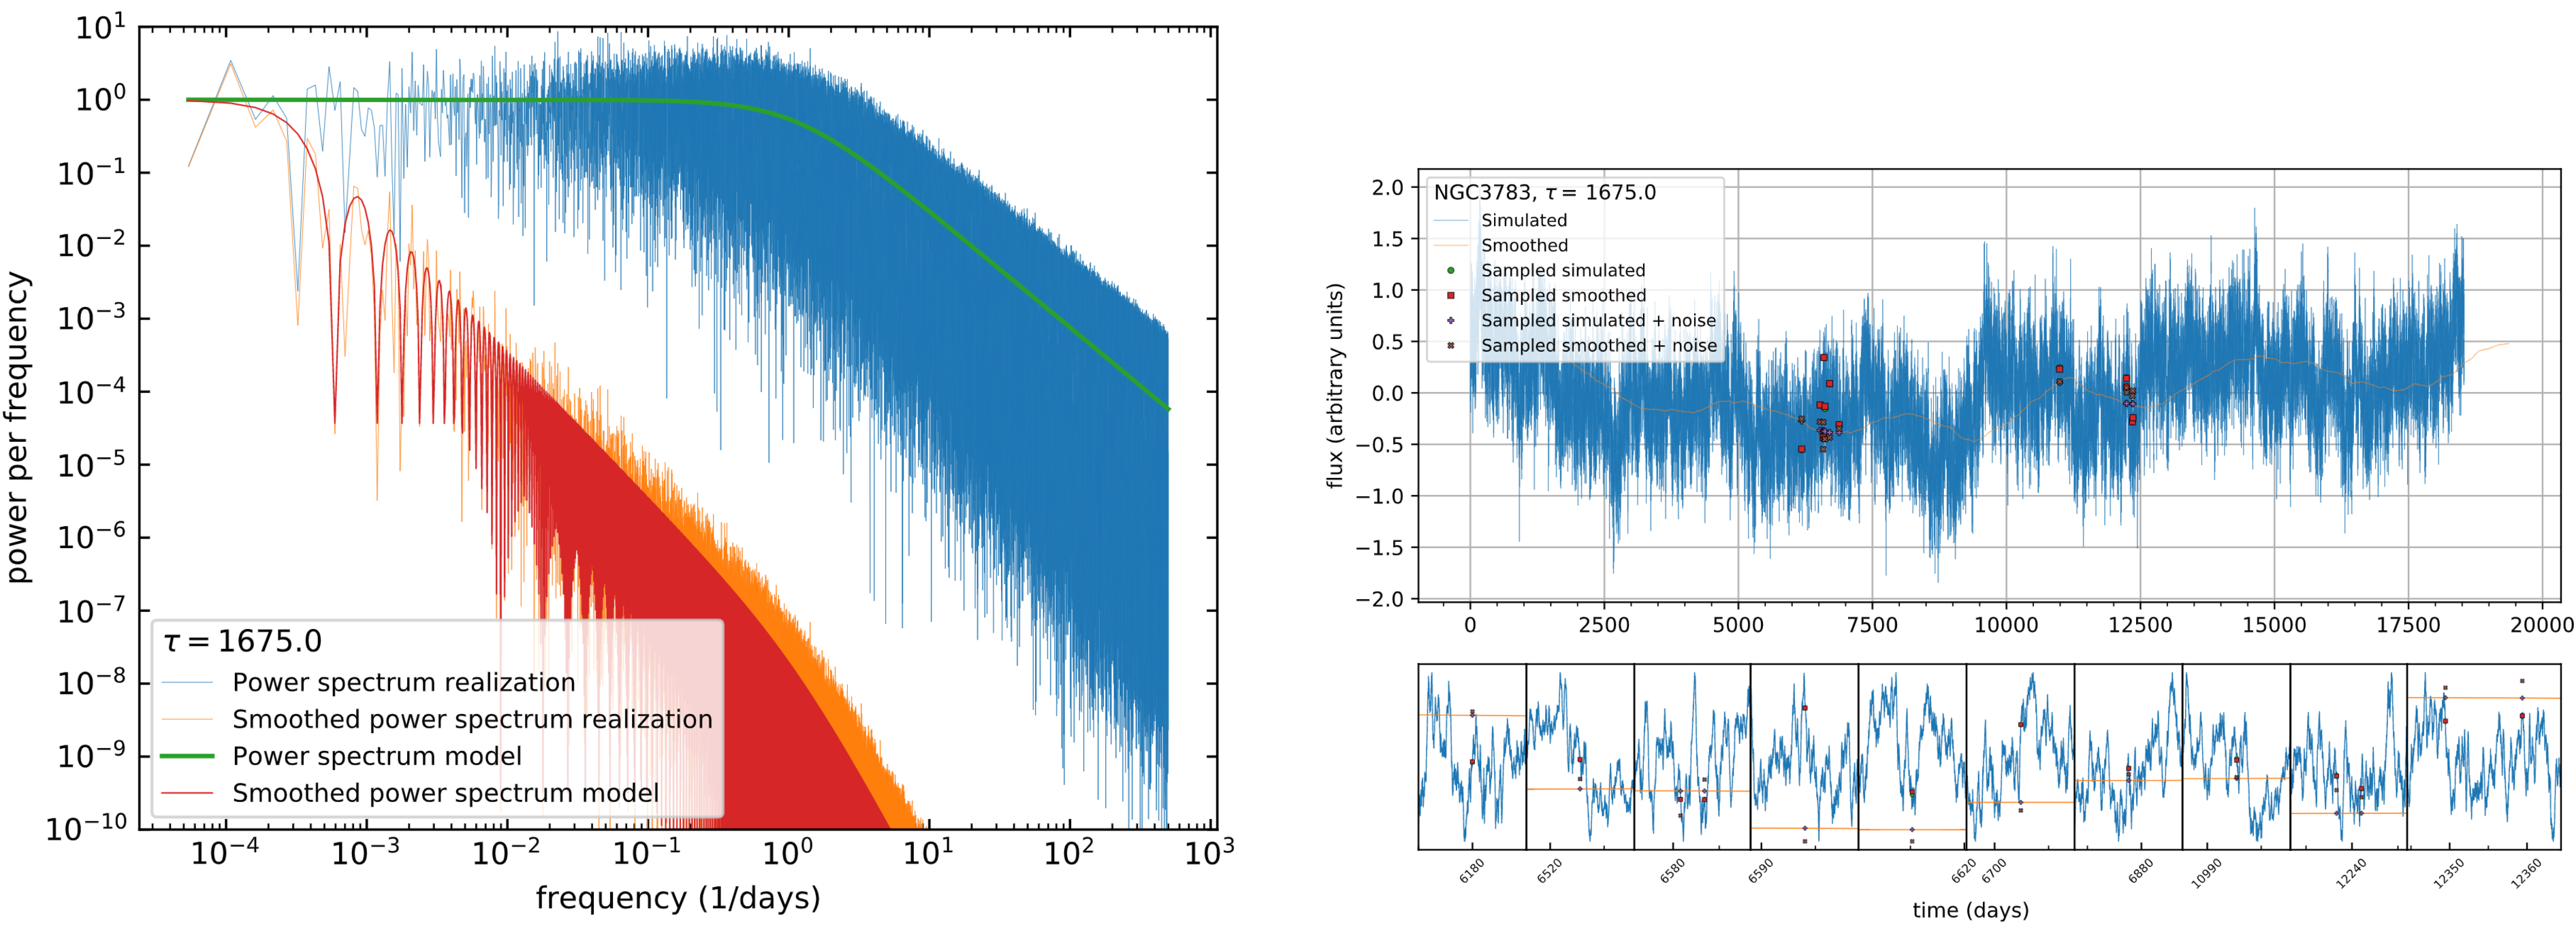
\includegraphics[width=\textwidth]{Figs/Chapter5/NGC3783/Screenshots/NGC3783_tau1675_LC_spectrum.pdf} \\
 % 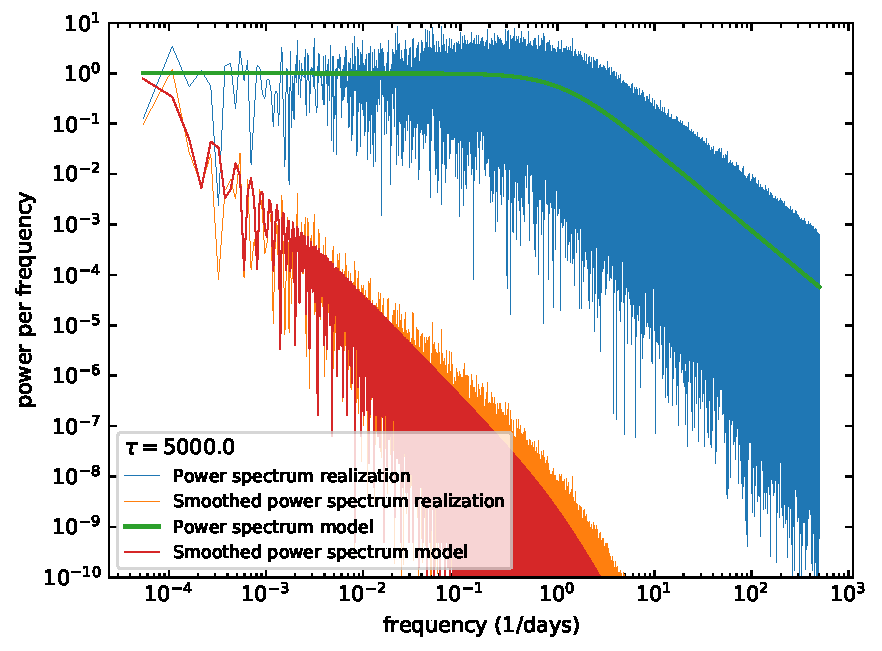
\includegraphics[width=0.49\textwidth]{Figs/Chapter5/NGC3783/power_spectrum_tau5000.0.pdf} \hfill 
 % 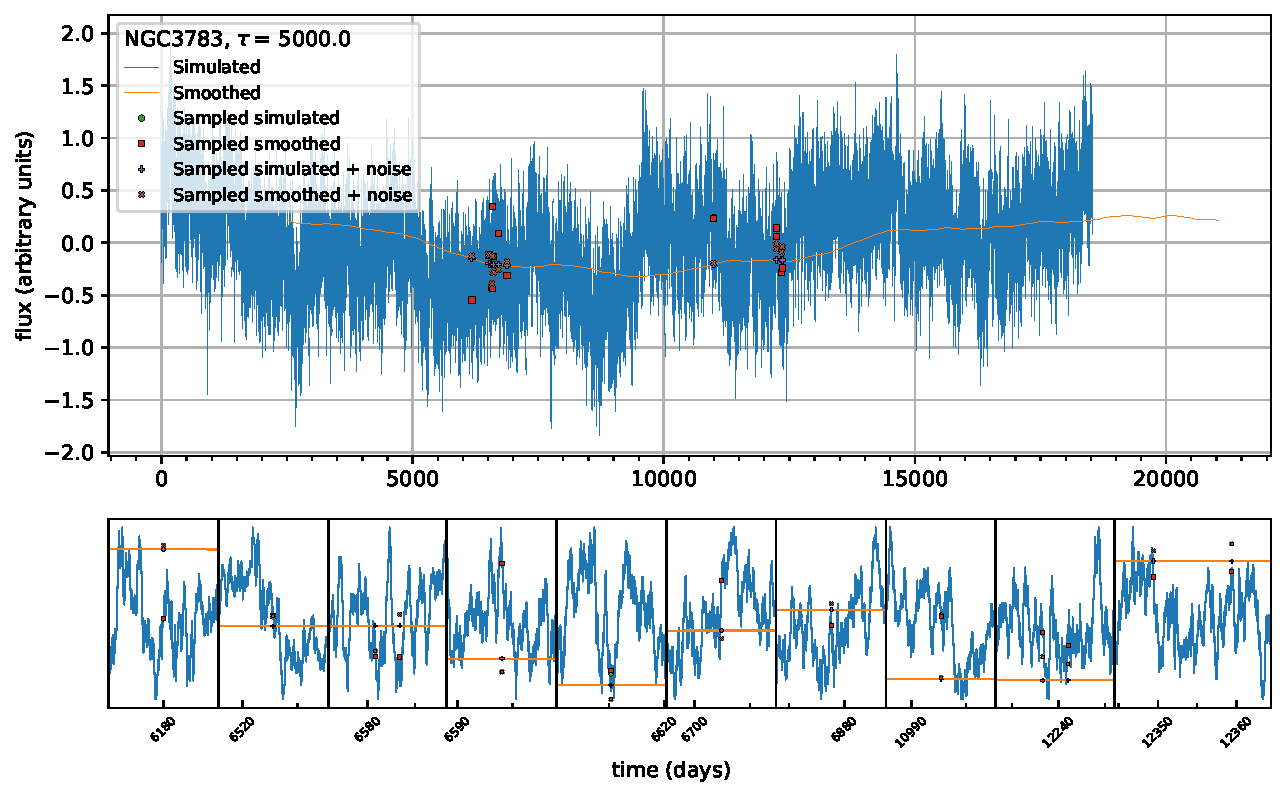
\includegraphics[width=0.49\textwidth]{Figs/Chapter5/NGC3783/sim_LC_tau5000.0_0_matrix.pdf} \\
  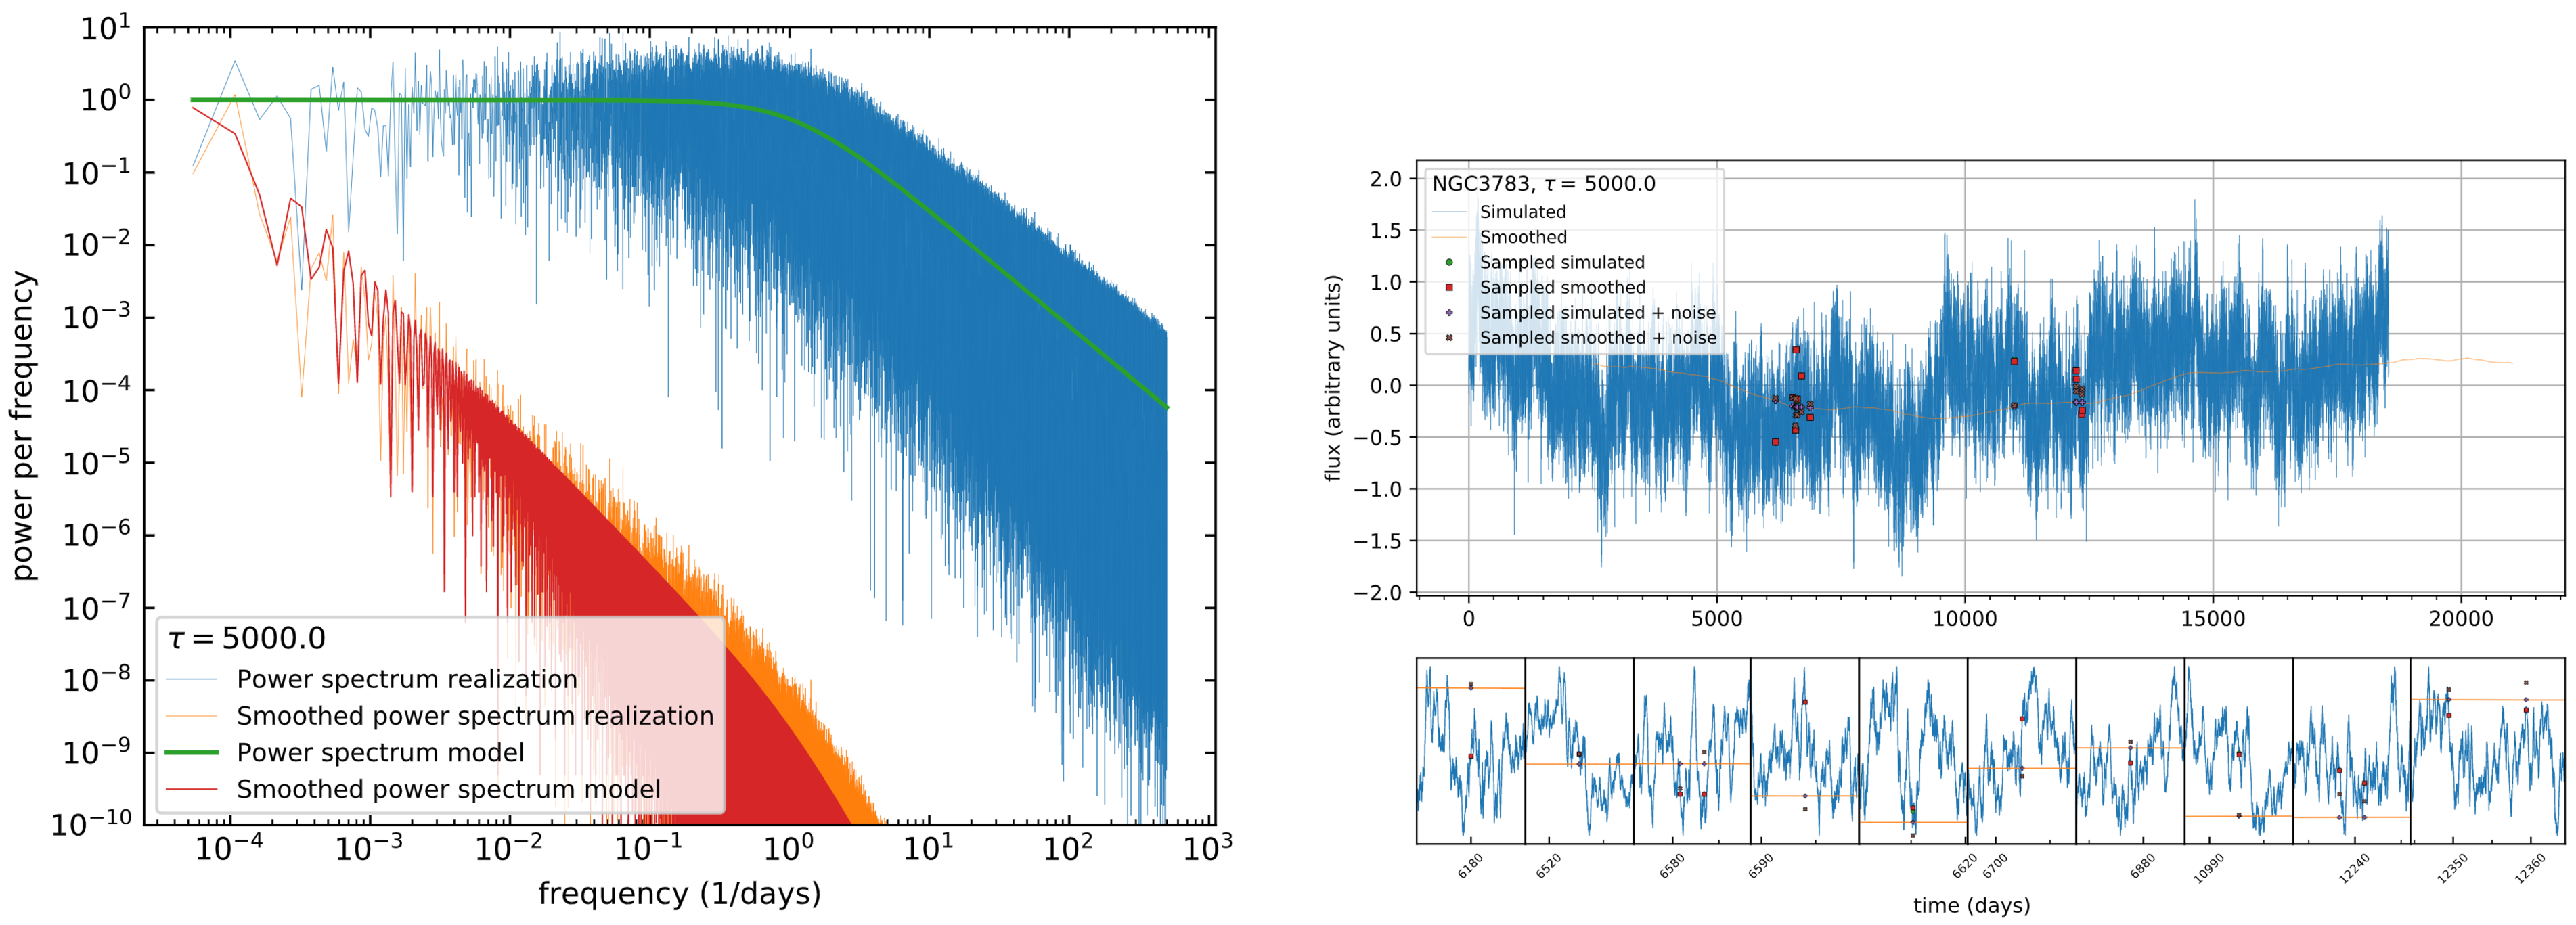
\includegraphics[width=\textwidth]{Figs/Chapter5/NGC3783/Screenshots/NGC3783_tau5000_LC_spectrum.pdf} \\
  \caption{Power spectrum NGC 3783}
    \label{fig:power_spectra_2_NGC3783}
  }
\end{center}
\end{figure}

\begin{figure}
\begin{center}
    {
  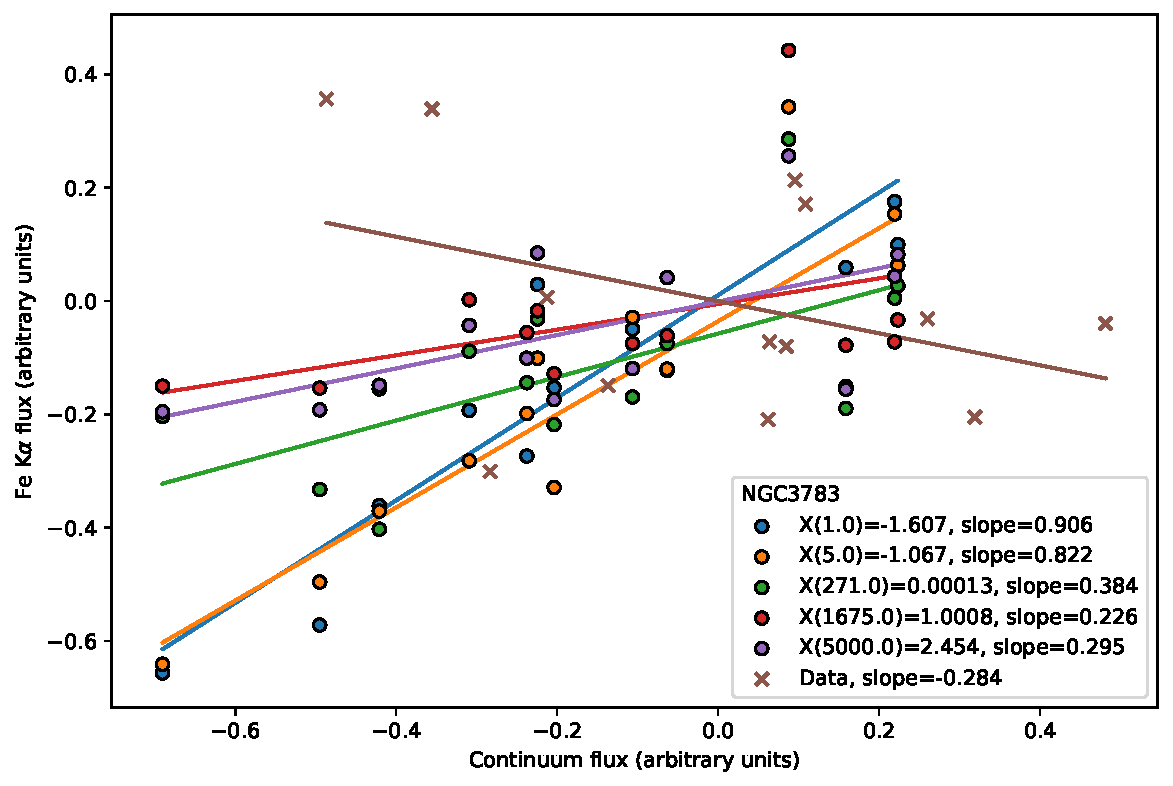
\includegraphics[width=0.7\textwidth]{Figs/Chapter5/NGC3783/Flux_flux_NGC3783.pdf} \hfill 
  \caption{Flux - flux plot NGC 3783}
    \label{fig:Flux-flux_NGC3783}
  }
\end{center}
\end{figure}



\begin{figure}
\begin{center}
    {
  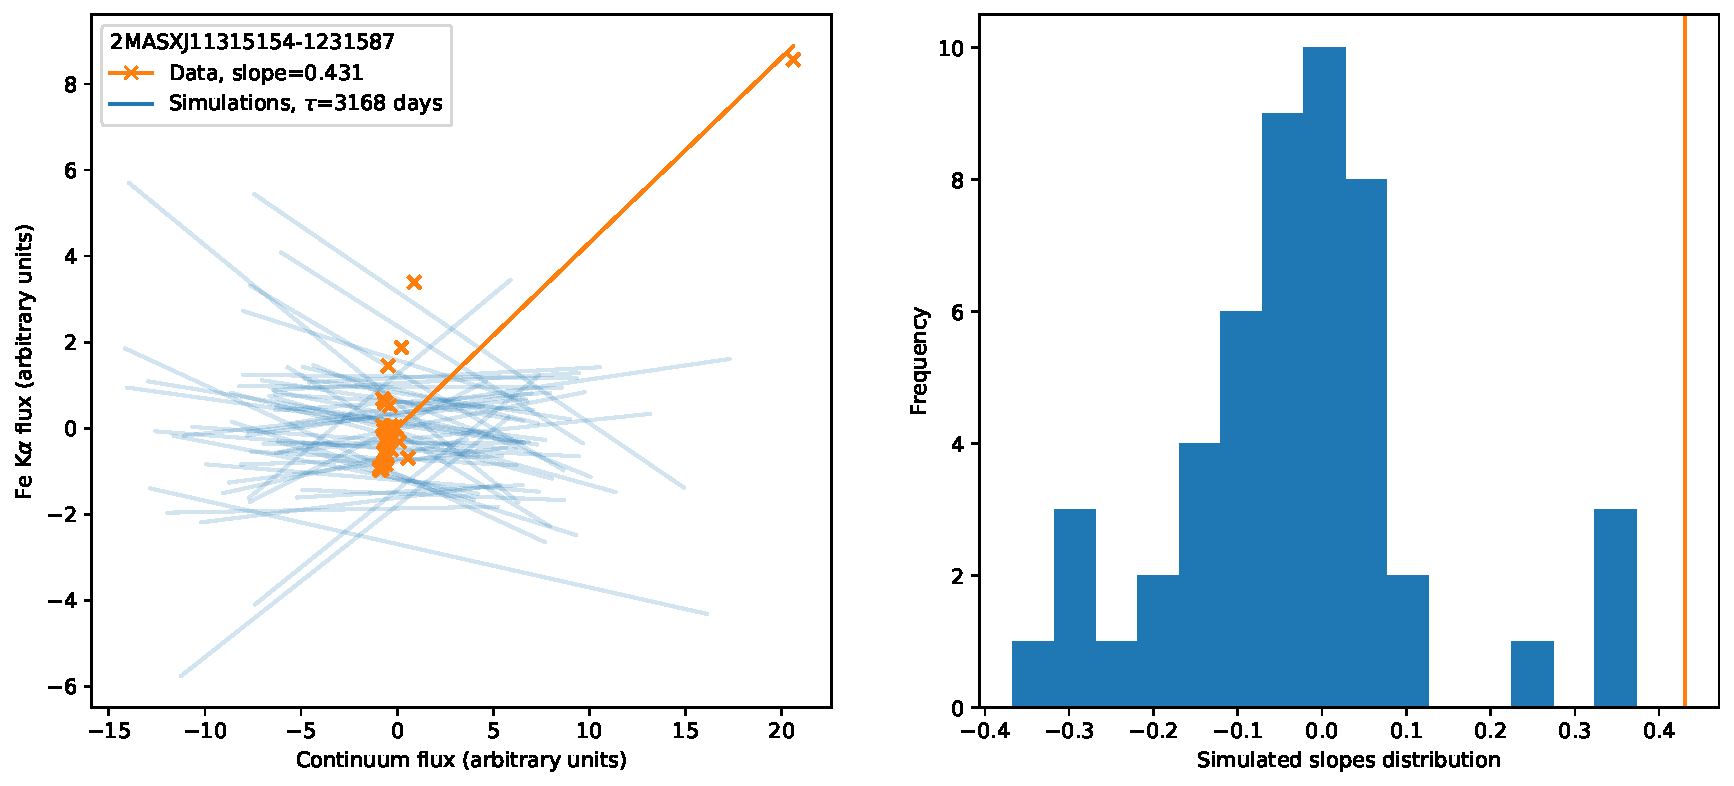
\includegraphics[width=\textwidth]{Figs/Chapter5/Flux_corr/Flux_flux_2MASXJ11315154-1231587_besttau.pdf} \\
  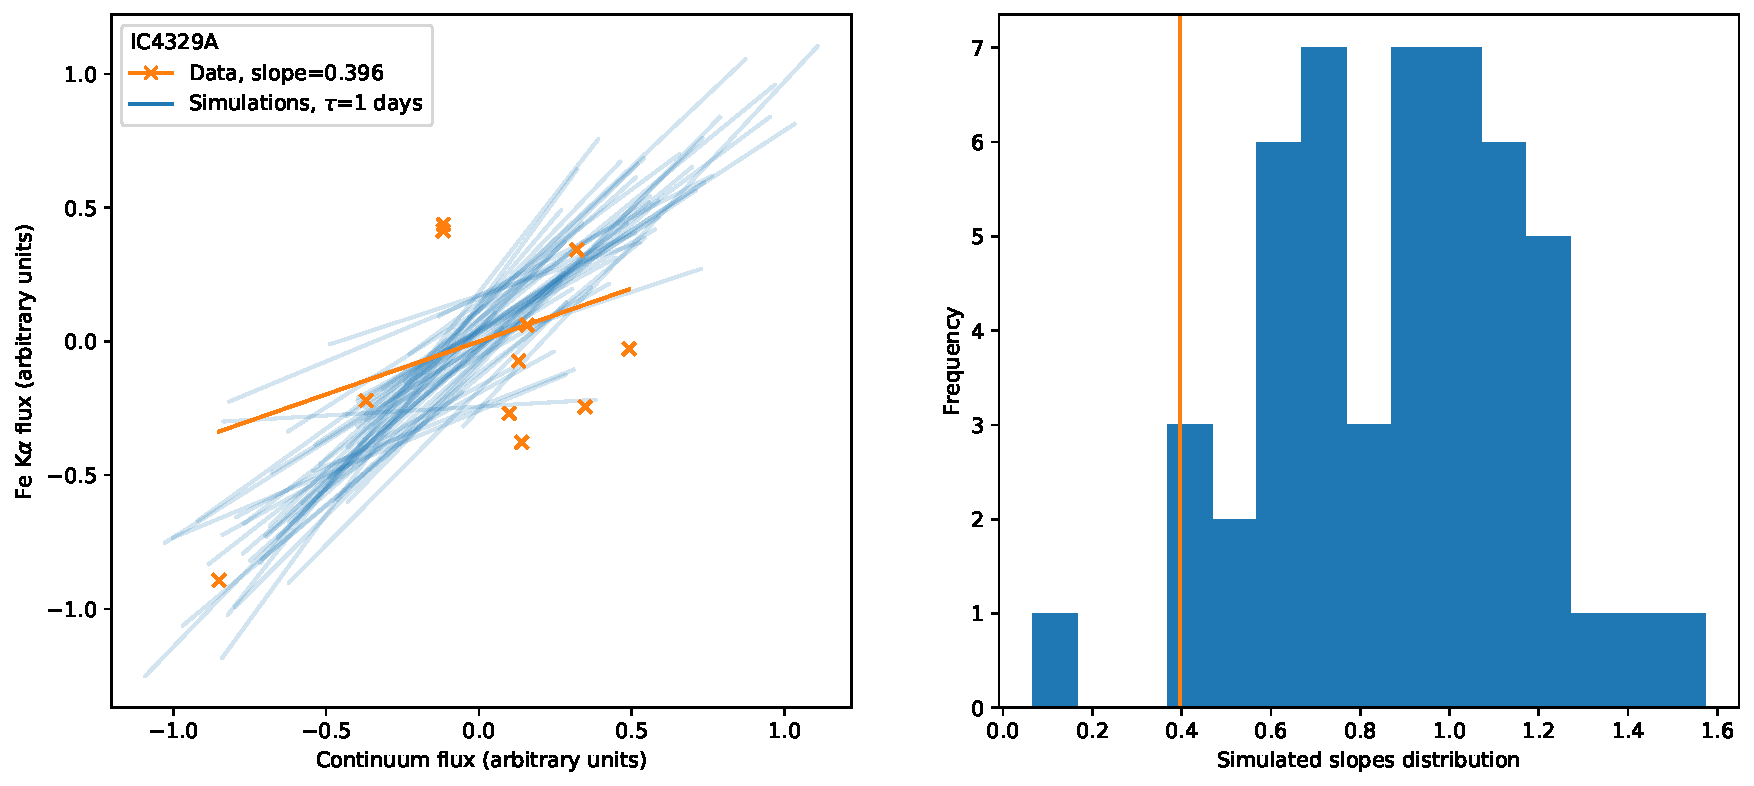
\includegraphics[width=\textwidth]{Figs/Chapter5/Flux_corr/Flux_flux_IC4329A_besttau.pdf} \\
  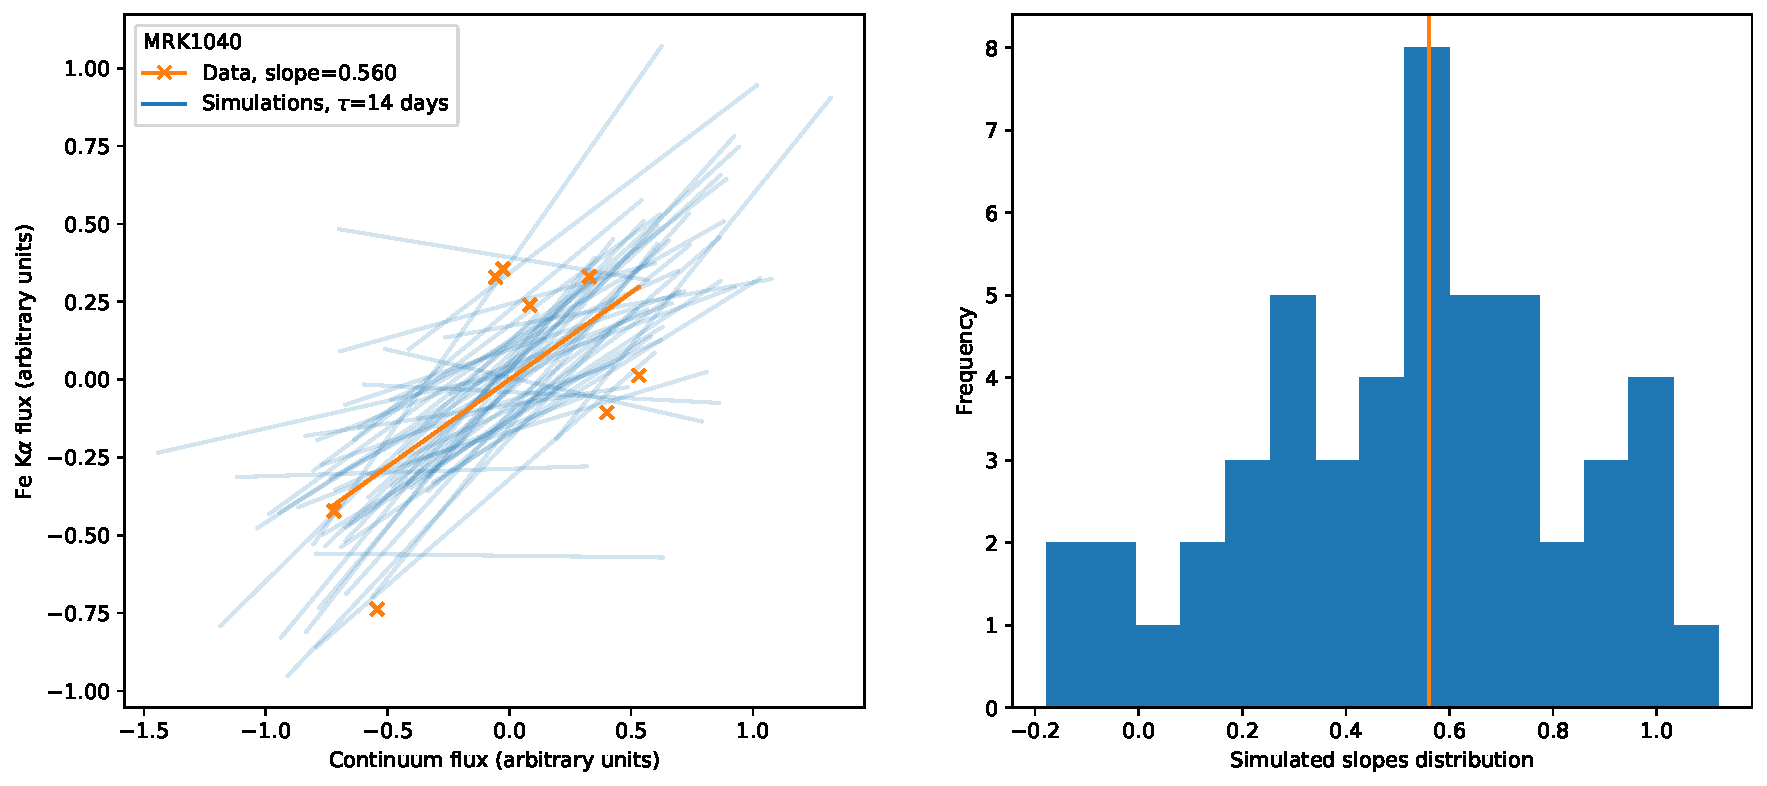
\includegraphics[width=\textwidth]{Figs/Chapter5/Flux_corr/Flux_flux_MRK1040_besttau.pdf}  \\
  \caption{Flux-flux correlation at best tau}
    \label{fig:Flux-flux_all_1}
  }
\end{center}
\end{figure}

\begin{figure}
\begin{center}
    {
  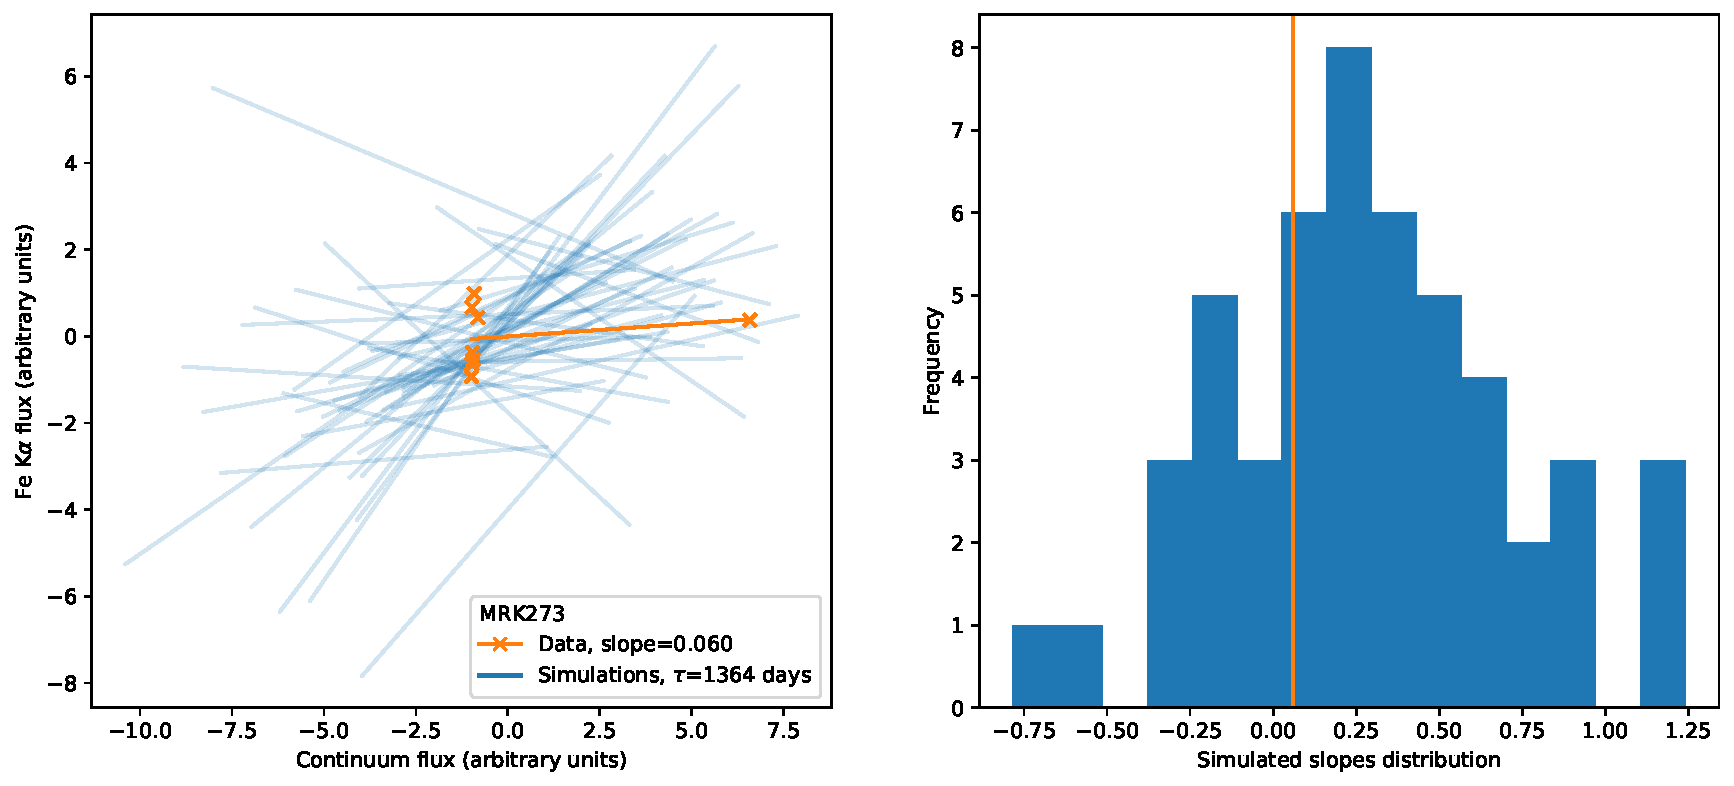
\includegraphics[width=\textwidth]{Figs/Chapter5/Flux_corr/Flux_flux_MRK273_besttau.pdf} \\
  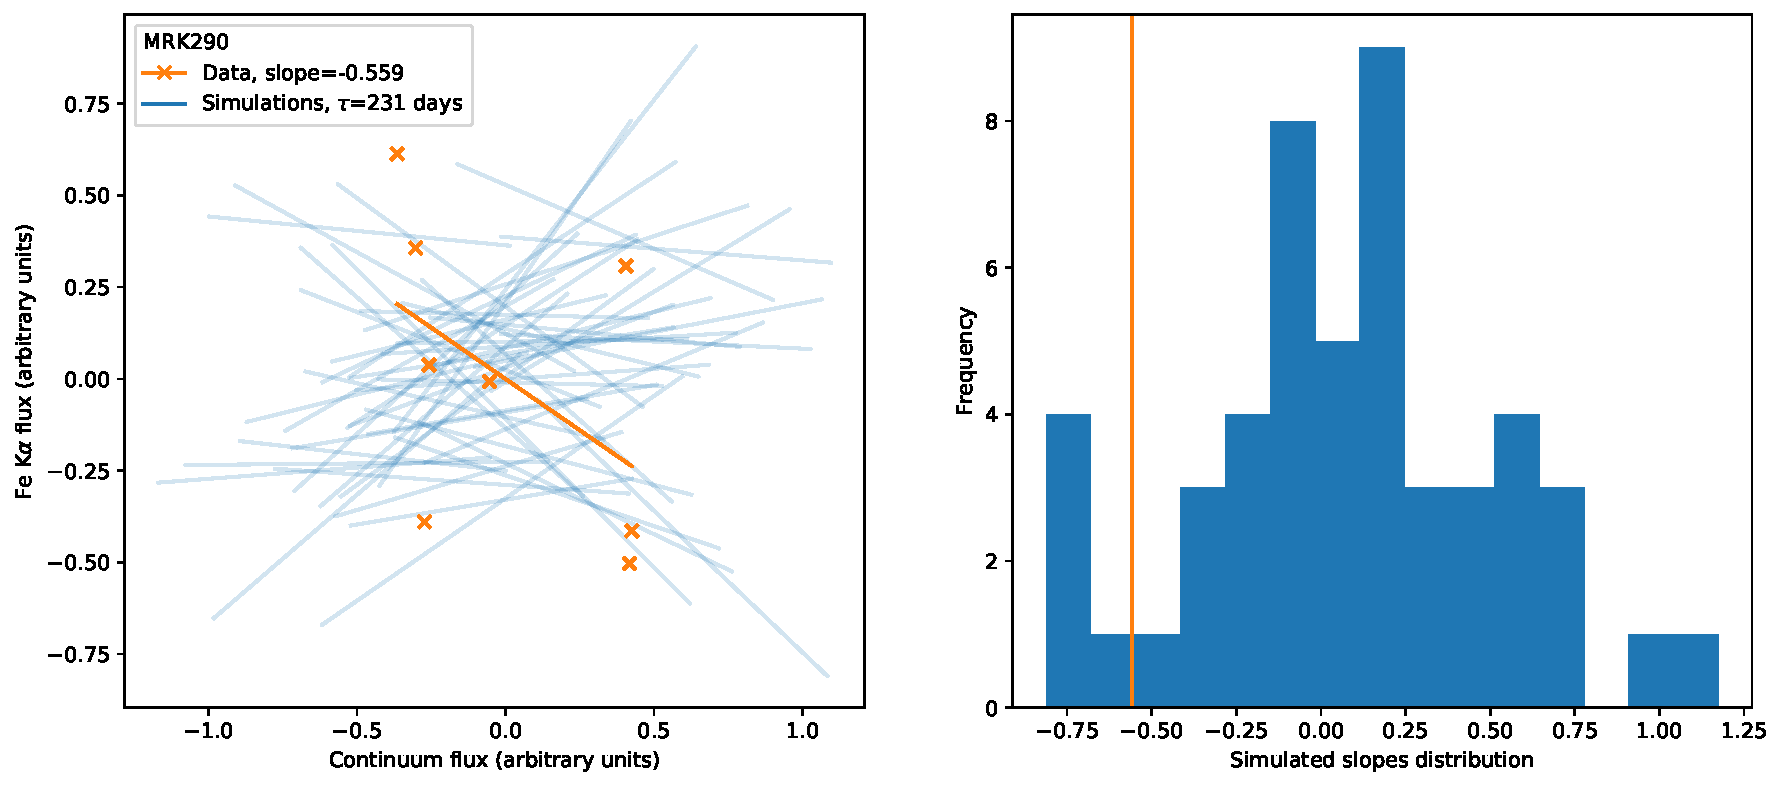
\includegraphics[width=\textwidth]{Figs/Chapter5/Flux_corr/Flux_flux_MRK290_besttau.pdf} \\
  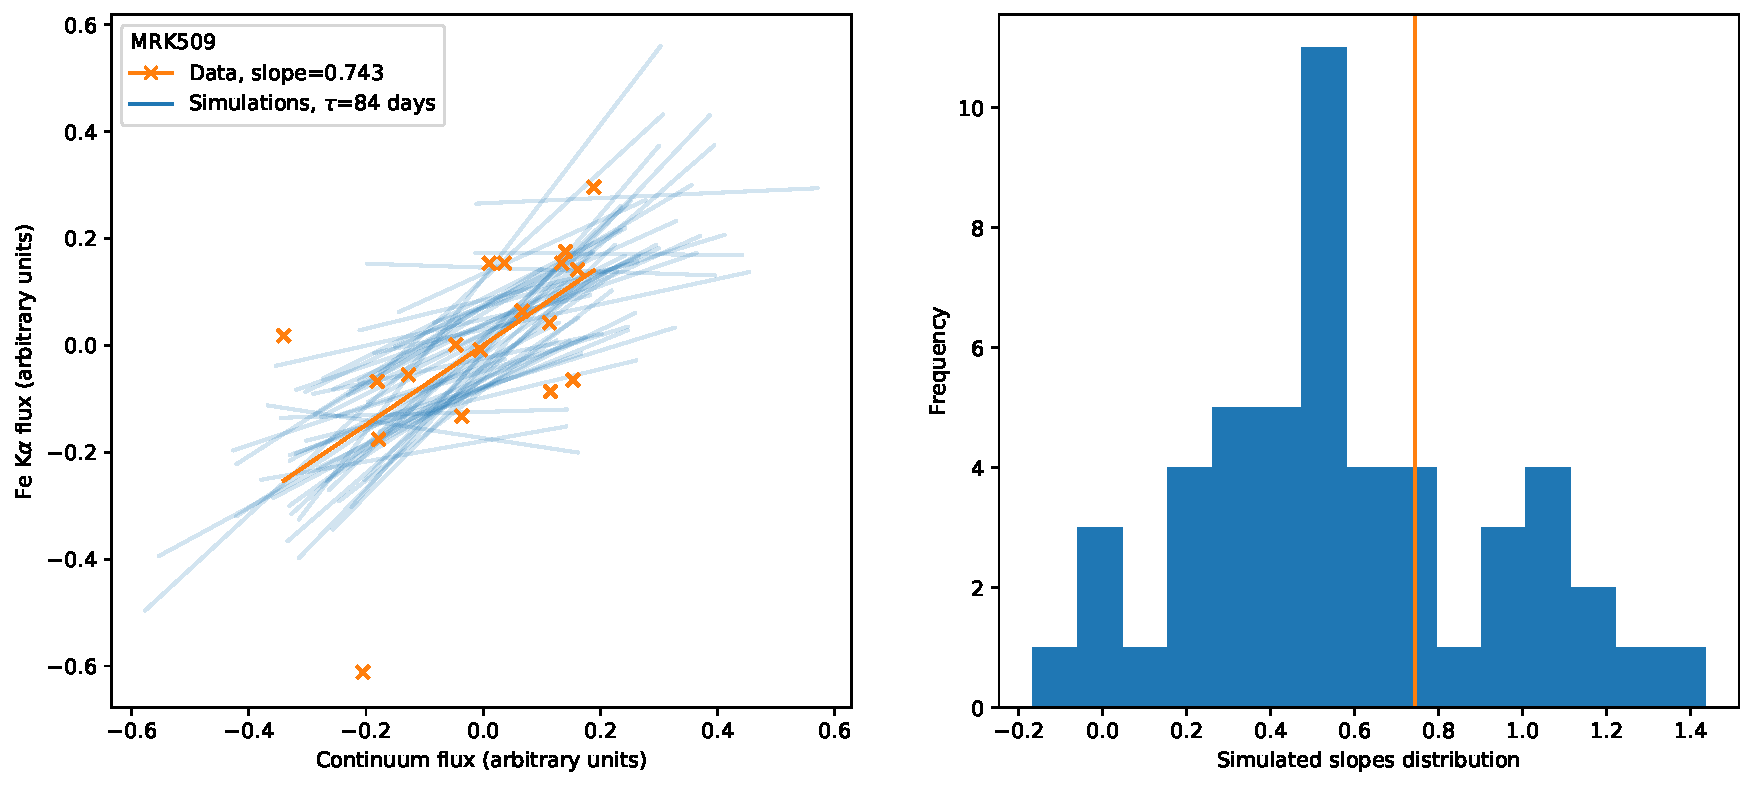
\includegraphics[width=\textwidth]{Figs/Chapter5/Flux_corr/Flux_flux_MRK509_besttau.pdf}  \\
  \caption{Flux-flux correlation at best tau}
    \label{fig:Flux-flux_all_2}
  }
\end{center}
\end{figure}

\begin{figure}
\begin{center}
    {
  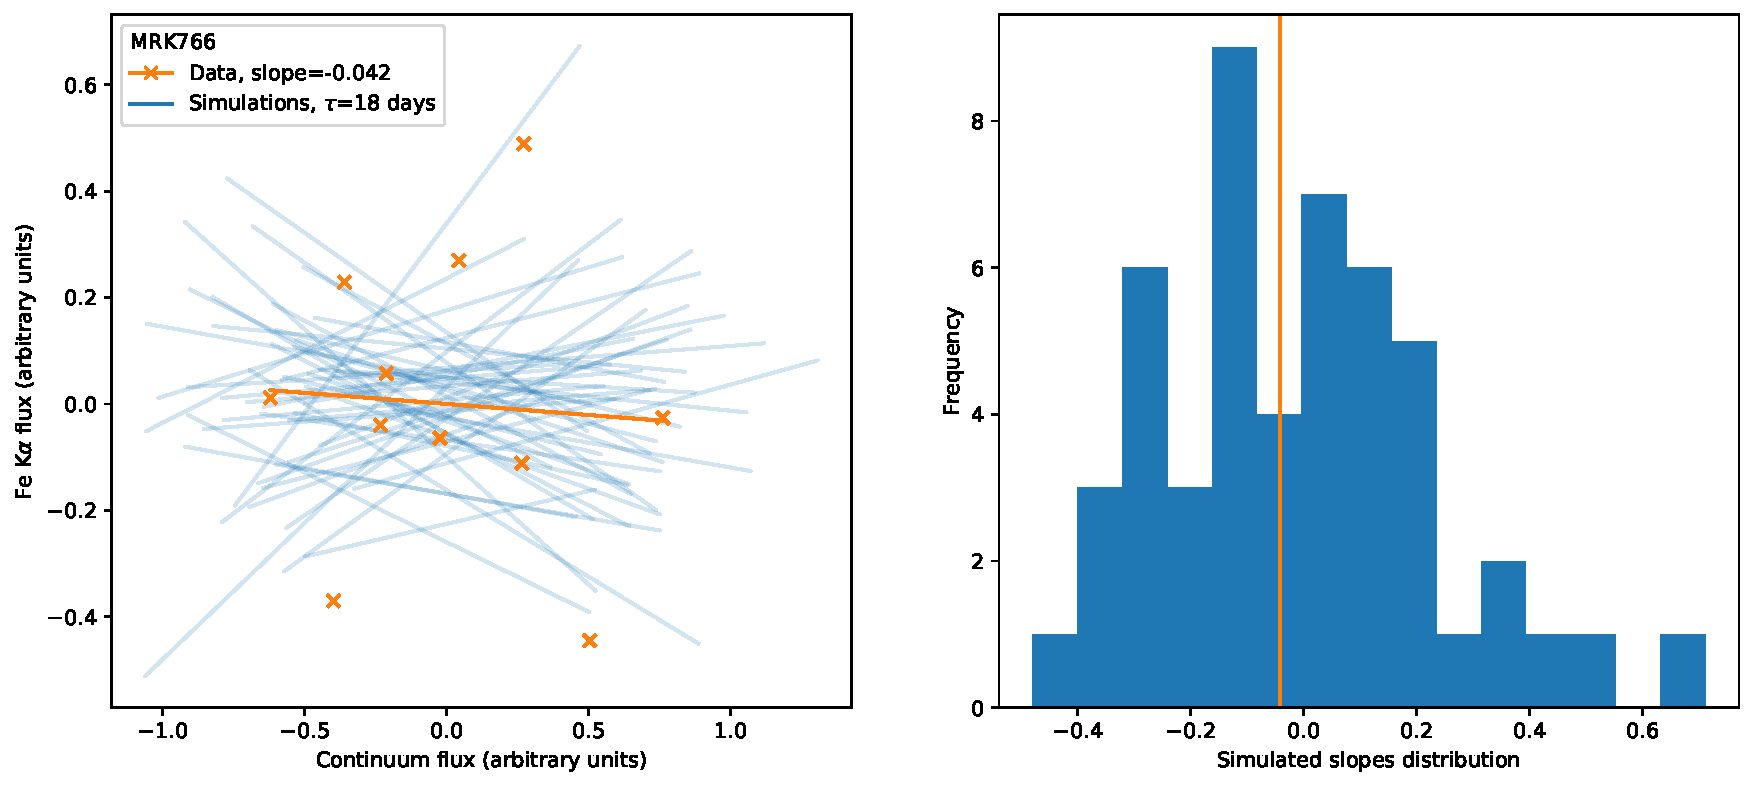
\includegraphics[width=\textwidth]{Figs/Chapter5/Flux_corr/Flux_flux_MRK766_besttau.pdf} \\
  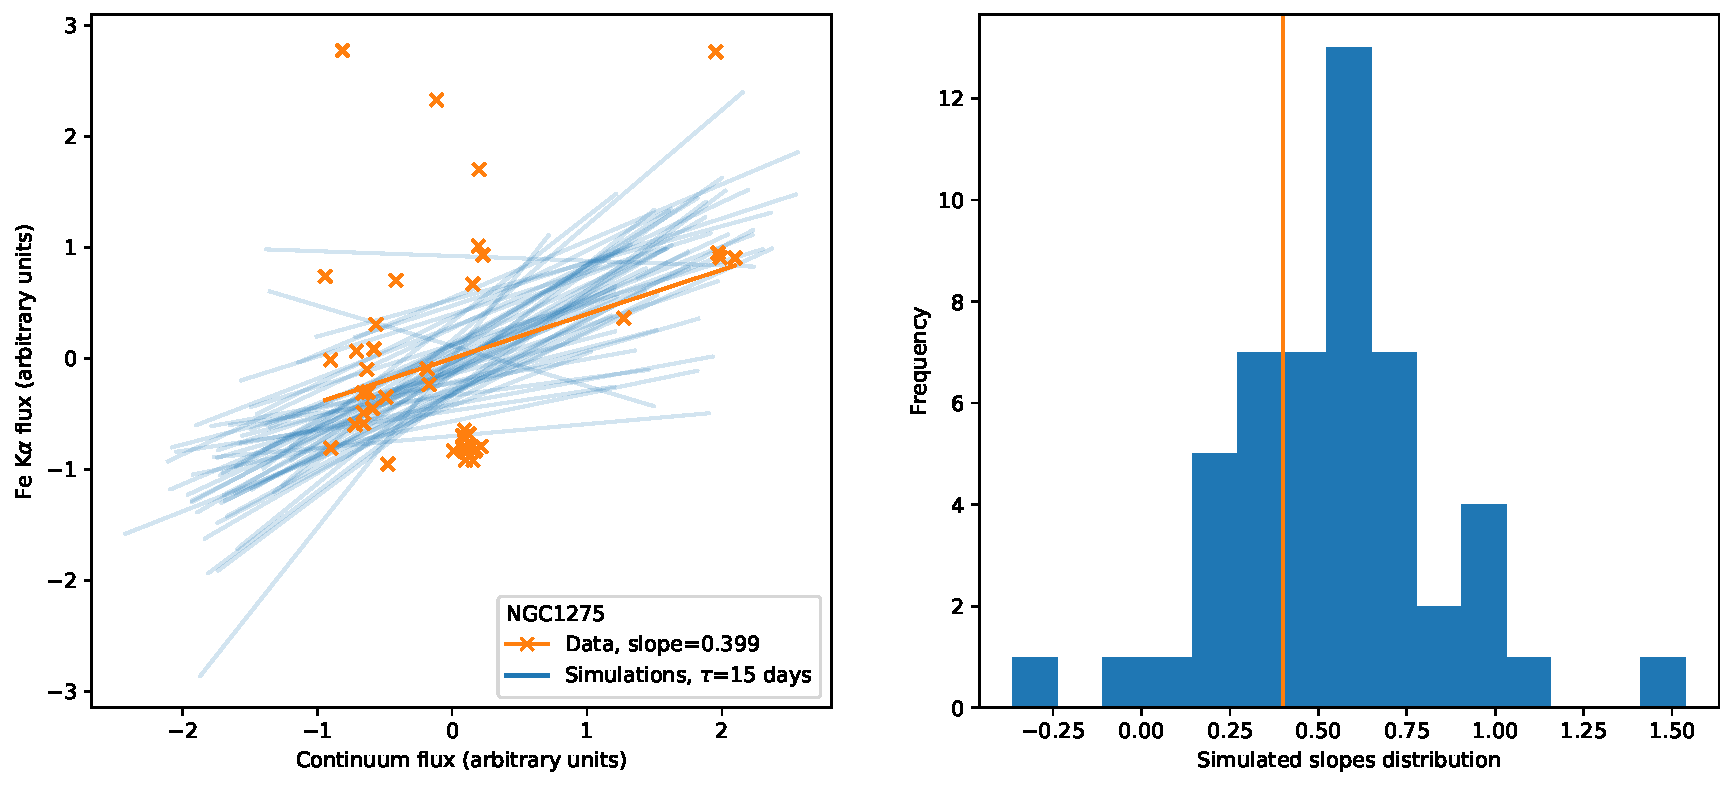
\includegraphics[width=\textwidth]{Figs/Chapter5/Flux_corr/Flux_flux_NGC1275_besttau.pdf} \\
  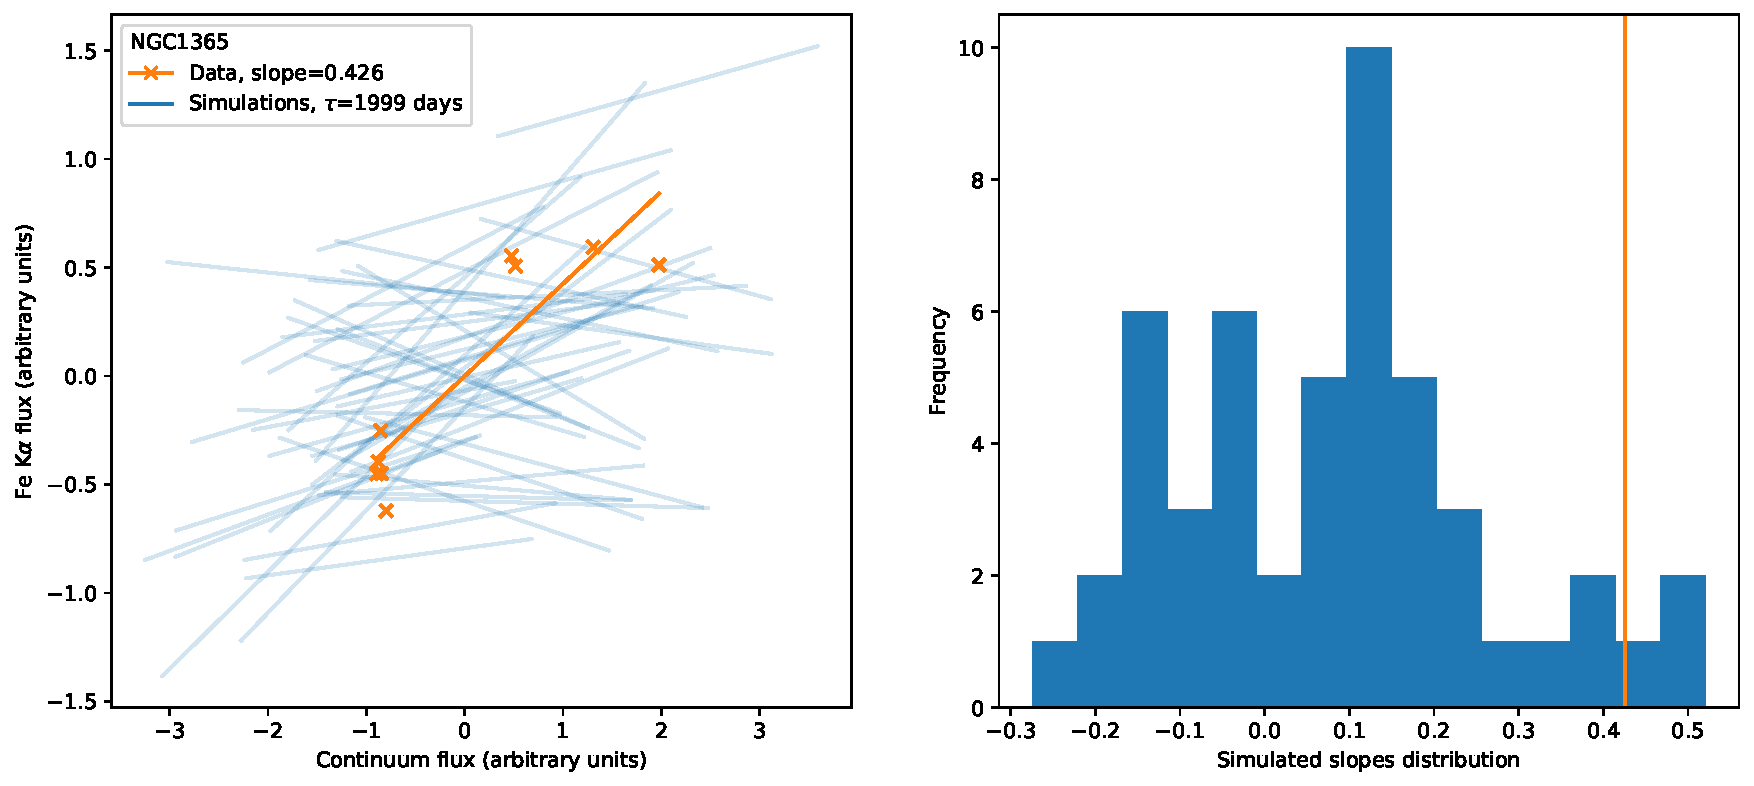
\includegraphics[width=\textwidth]{Figs/Chapter5/Flux_corr/Flux_flux_NGC1365_besttau.pdf}  \\
  \caption{Flux-flux correlation at best tau}
    \label{fig:Flux-flux_all_3}
  }
\end{center}
\end{figure}

\begin{figure}
\begin{center}
    {
  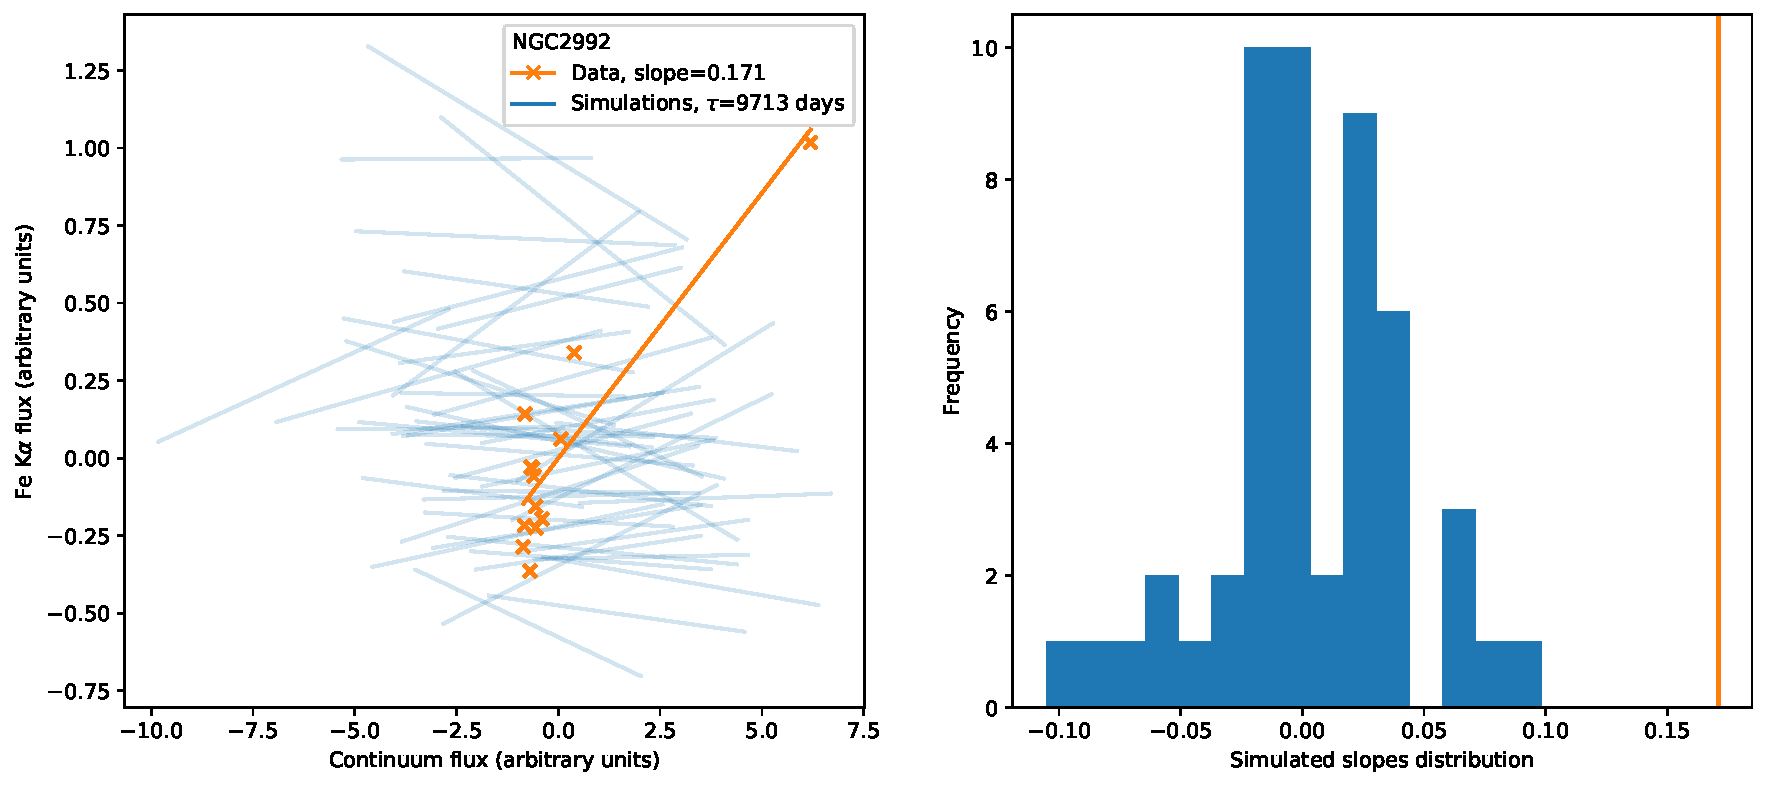
\includegraphics[width=\textwidth]{Figs/Chapter5/Flux_corr/Flux_flux_NGC2992_besttau.pdf} \\
  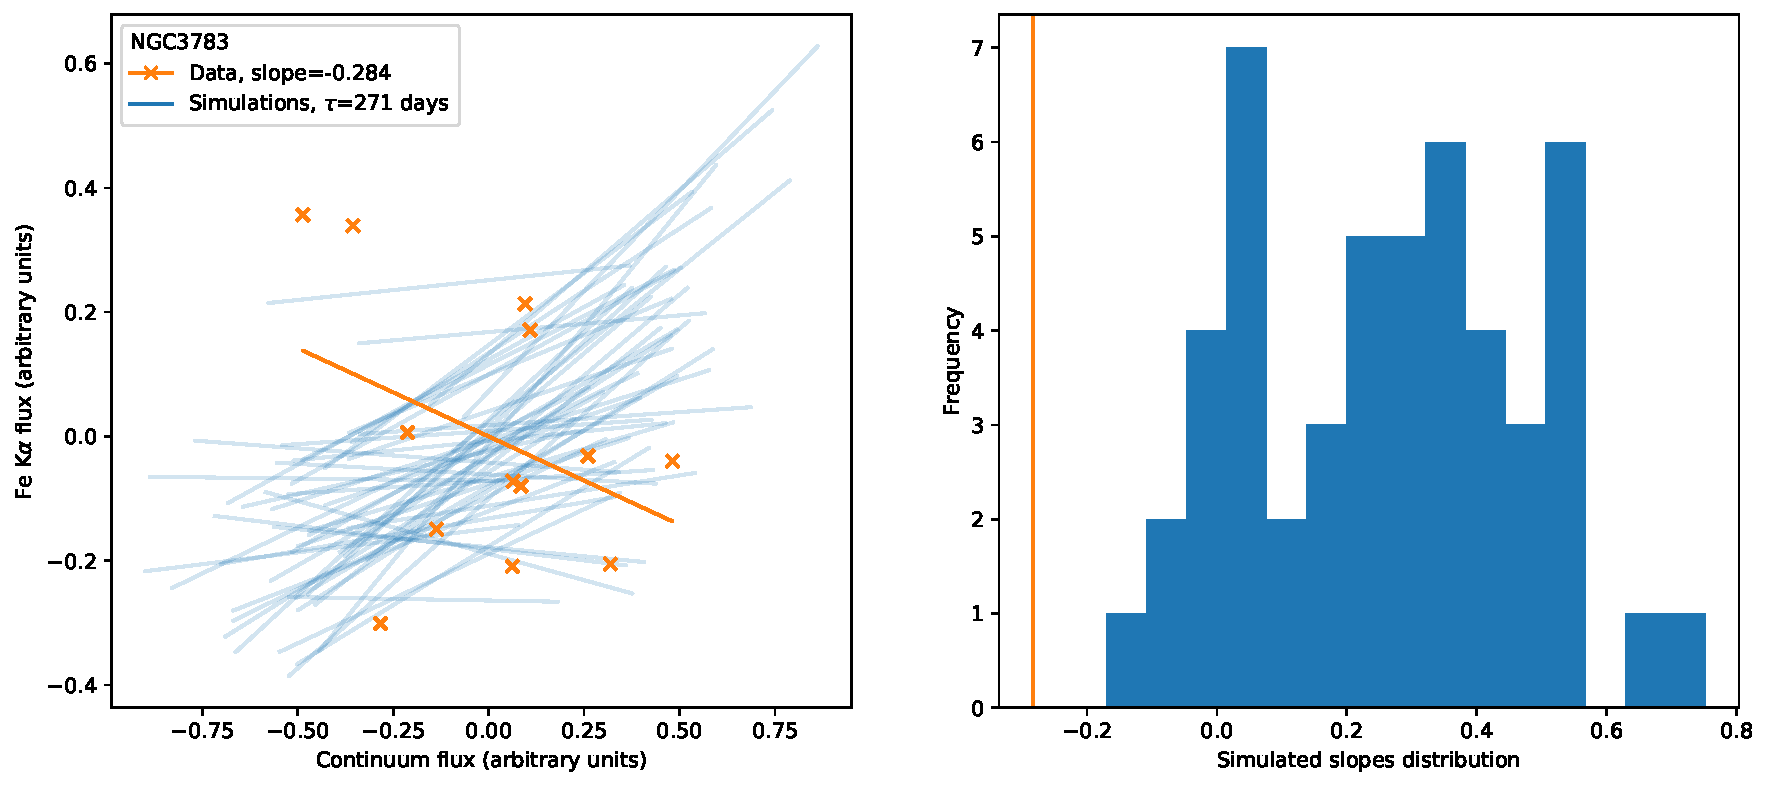
\includegraphics[width=\textwidth]{Figs/Chapter5/Flux_corr/Flux_flux_NGC3783_besttau.pdf} \\
  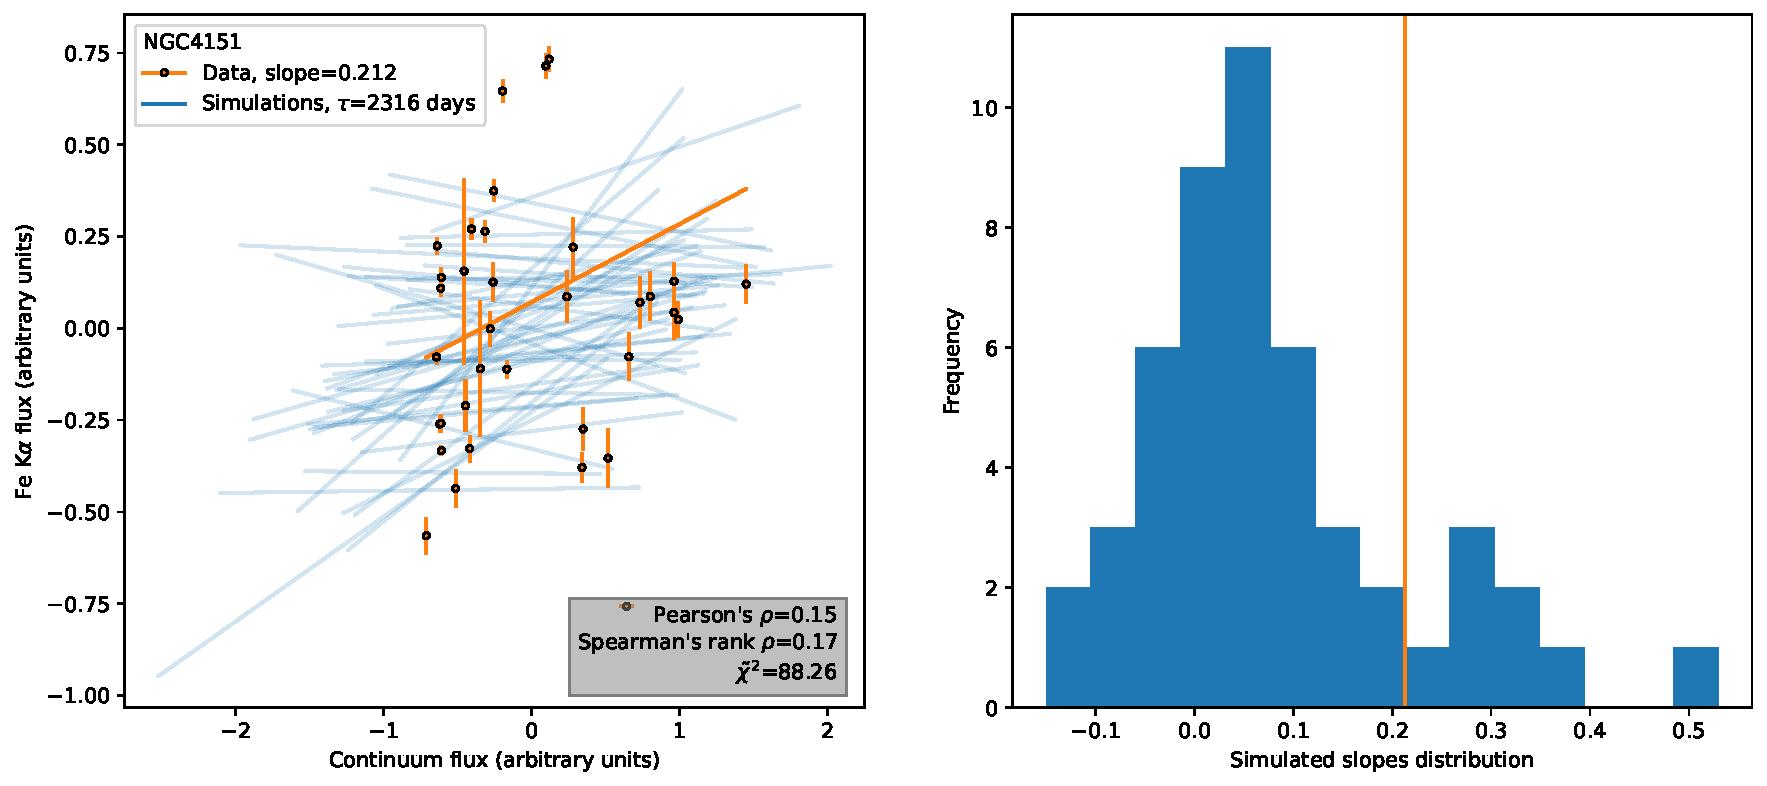
\includegraphics[width=\textwidth]{Figs/Chapter5/Flux_corr/Flux_flux_NGC4151_besttau.pdf}  \\
  \caption{Flux-flux correlation at best tau}
    \label{fig:Flux-flux_all_4}
  }
\end{center}
\end{figure}

\begin{figure}
\begin{center}
    {
  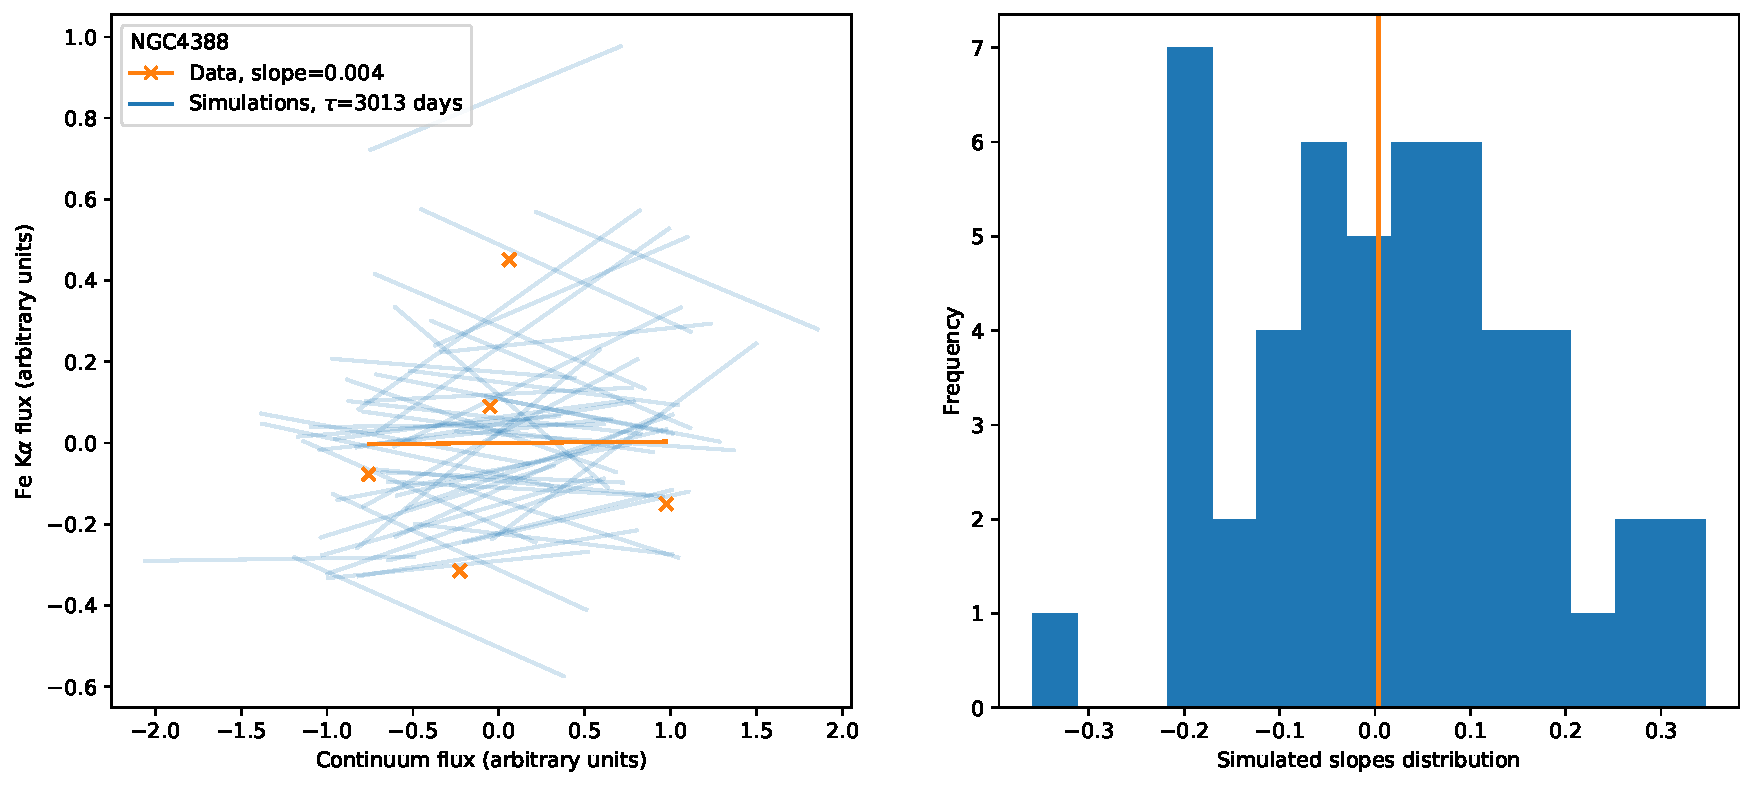
\includegraphics[width=\textwidth]{Figs/Chapter5/Flux_corr/Flux_flux_NGC4388_besttau.pdf} \\
  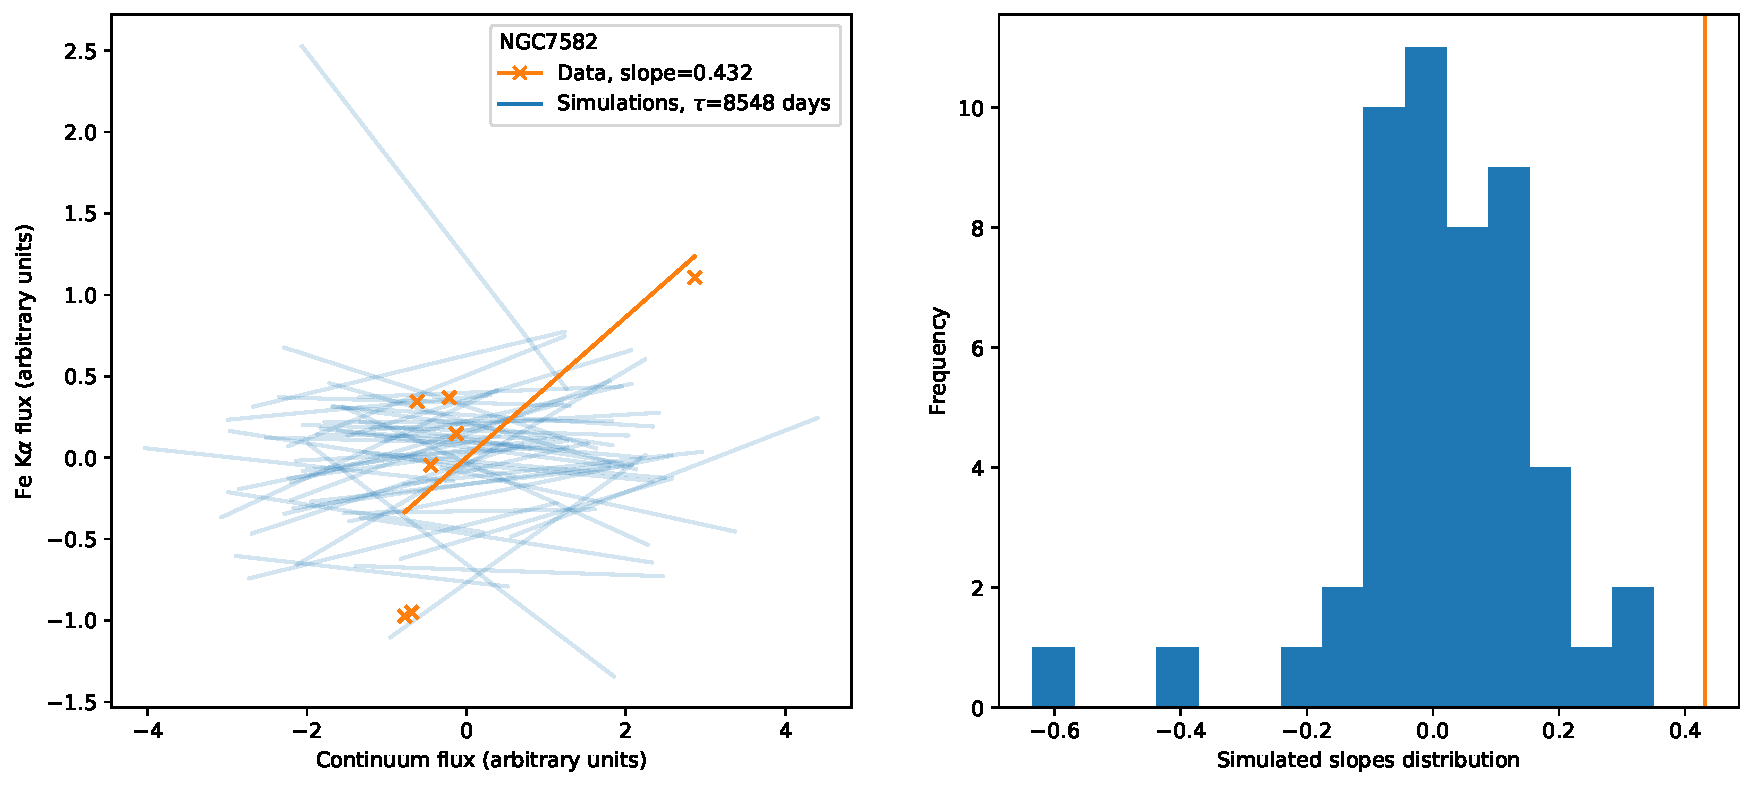
\includegraphics[width=\textwidth]{Figs/Chapter5/Flux_corr/Flux_flux_NGC7582_besttau.pdf} \\
  \caption{Flux-flux correlation at best tau}
    \label{fig:Flux-flux_all_5}
  }
\end{center}
\end{figure}

\iffalse
Comments:
- light curve time resolution: same number of decimals as \verb+decimals=-int(np.floor(np.log10(abs(1/nu/100))))+ \\
- rescaling    \verb+average_cont = lc['flux_cont(ph/cm^2/s)'].mean()+, 
   \verb+lc['flux_cont(ph/cm^2/s)']=(lc['flux_cont(ph/cm^2/s)']-average_cont)/average_cont+ and same for line (but then I multiply them again for the average....)\\
- explore a range of taus $\tau$, 500 simulations per each \\
- simulated light curve is \verb+n_length*duration+ of the data and is \verb-np.max(taus)/duration+1- if $dt=1e-4$ or \verb+n_length=2+ if $dt=1e-3$ or \verb-max([3,np.max(taus)/duration+1])- if $dt>1e-3$.\\
- Simulation equations, with Re and Im randomly generated numbers with a Gaussian distribution
\begin{equation}
    SimPS_+=(Re+1j*Im)*(PS/2)^{0.5}, \;
    SimPS_-=(Re-1j*Im)*(PS/2)^{0.5}
\end{equation}
- Filter with top hat function in Fourier space, which corresponds to a $\sinc$ function:
- We apply inverse fast Fourier transform (IFFT) to the total SimPS composed of a $0+0j$,$SimPS_+$, and $SimPS_-$. We do the same for SimPSsmooth. \\
- The real part of the result of the two IFFTs is our simulated light curve \\
- Sampling \\
- Noise \\
- Variances - $\xi$ \\
- we want to compare the $\xi_{\rm data}$ with the $\xi_{\rm sim}$ 
- we need to find a $\xi_{\rm sim}$ that matches $\xi_{\rm data}$ such that
\begin{equation}
    {\rm X}(\tau)=\frac{\xi_{\rm data}-<\xi_{\rm sim}>}{(\xi_{\rm sim})_{rms}}=0
\end{equation}
- that tau is the size of the reprocessor\\
- Given how X is defined X$=\pm1$ correspond to $1\sigma$ intervals.\\
- Estimate X \\
- Use Newton's method for finding the root with a tolerance of tol=0.005 and a min time res of 1 day\\
- Run Newton method in order to find also $X=\pm1$ with the same tolerance\\
- Show plots with X of the entire sample
- explain results 
\fi


\section{Discussion}
After constraining the size of the reprocessor for a portion of the galaxies in our sample, we want to find a relation with AGN properties. 
A possibility is for the reprocessor size to scale with the mass of the black hole ${\rm M}_{\rm BH}$. In fact, the size of the circumnuclear environment around the black hole scales, at least partially, with the ${\rm M}_{\rm BH}$, e.g. the Schwarzschild radius, the sphere of influence, internal dust radius, the broad line region, so it seems viable for the material reprocessing the X-ray emission from the corona to increase its size with ${\rm M}_{\rm BH}$.

In Figure~\ref{fig:tau_mass_corr} we show all the reprocessor sizes in light day units, with their confidence ranges, as a function of ${\rm M}_{\rm BH}$ (we remind the reader that the diameter of the reprocessor corresponds to $d=c\tau$). Since we are considering only a range of 1-10,000 light days in size, for the cases where we couldn't constrain the $1\sigma$ ranges (see sources with missing $\tau_{inf}$ and/or $\tau_{sup}$ on Table~\ref{tab:taus}) we are showing error-bars covering from the best size $\tau*$ to the lower/upper extreme of the $\tau$ range. Along with these we also show a log-log best fit to the data which shows a slope $0.66\pm0.53$. With the help of the Pearson's correlation coefficient, the Spearman's rank and the $\tilde\chi^2$ we see that there is a mild positive correlation in this relation with a large scatter of $\sim1 dex$.

This seemingly weak correlation though, is an interesting starting point that poses this analysis method as a promising one. In fact it allows to place constraints on the size of the reprocessor of quite a few sources and sets a good base for future monitoring campaigns. In fact, by placing lower limits on the size of the reprocessor we can define good sampling frequencies and by placing upper limits we can define a convenient duration of the monitoring campaign in order to measure the lag between the two light curves. 
Whenever an upper limit is not present, or when this is $\gtrapprox10^3$, it suggests that our kind of analysis based on the measure of the smoothing in the \kalfa{} light curve, is still the best way to go, as very long monitoring campaigns are time expensive and would require years or even decades to lead to a lag measurement. Repeating this analysis with an adequate amount of data-points would certainly allow for a better estimate of the reprocessor size.

%- some galaxies have nuclear reprocessors, others have extended ones

Another possibility for future work is an analysis of the correlation between AGN type properties and $\xi$, as other physical factors may be influencing the emissions and therefore the measured size of the reprocessor, thus causing the scatter in the ${\rm M}_{\rm BH} - \tau$ relation. As already mentioned, the light curves of radio loud sources may be affected from beamed X-ray emission leading to light curves that do not trace the same variations. Another behavior we might expect is from Compton-thick AGN, which should have reflection-dominated continua with little variation, and thus our simple X-ray spectral fitting approach would measure the flux of this relatively static component causing a $\xi<1$. Another example yet is the case of changing look AGN, where covering factor changes may increase the continuum variability from the observers point of view, but not necessarily from the point of view of the whole reflector.
\begin{figure}
\begin{center}
    {
  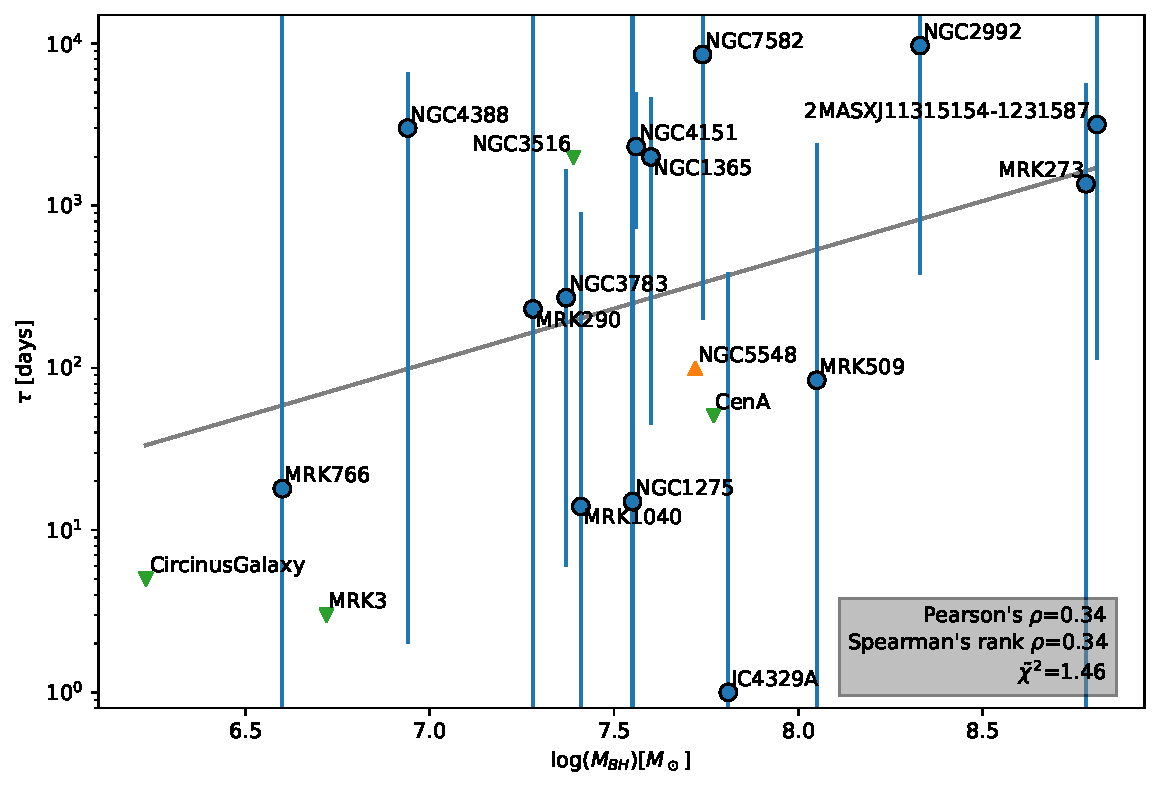
\includegraphics[width=\textwidth]{Figs/Chapter5/tau_mass_corr.pdf} \hfill 
  \caption{Correlation between black hole mass (${\rm M}_{\rm BH}$) and reprocessor size $\tau$ expressed in light days. The $y$ axes is limited to the range of light days considered in our work, $1-10,000$, and sources with unconstrained upper/lower limits have error bars extending all the way to the extremes of the plot.}
    \label{fig:tau_mass_corr}
  }
\end{center}
\end{figure}

\section{Conclusions}
In this Chapter we have used simulations in order to study the distribution of X-ray reprocessing gas (\emph{ the reprocessor}) in the active nuclei of a sample of local host galaxies. 
In our simple model we assumed that the X-ray continuum emission comes from the AGN corona and is then reprocessed by a spherical thin shell of gas around it, which causes a delay and a damping of the variations of the continuum in a way that depends on the distance between the corona and the reflector. In order to reproduce the behavior of this setup we simulated the X-ray light curves from the continuum starting from red noise in Fourier space following a power spectrum based on physical parameters of our sources, and the reflected component was obtained from the same light curve, which was smoothed and delayed in time.

The sample in this study was not observed through specific monitoring campaigns aimed at this kind of study, but we used archival data which allowed to retrieve light curves with few data-points observed through several years with irregular sampling. This did not allow to estimate a lag between the light curves but only to determine the variability reduction in amplitude caused by the reprocessor on the reflected component.

This simple modeling allowed us to completely constrain the size of the reprocessor for 4 sources in our sample and to determine at least a lower or upper limit size for 13 of them. For the remaining part of the sample, we either didn't have enough data points to correctly estimate the variability reduction, or the data quality was insufficient, or our model is too simple and does not apply to some individual source. Our resulting reprocessor estimates are still a promising starting point to design future monitoring campaigns that will be more effective at constraining the size of the reprocessor and may even be able to determine a lag between the light curves.

We found a correlation between the size of the reprocessor and the black hole mass ${\rm M}_{\rm BH}$ in our sample, which is consistent with other AGN properties which scale with the mass of the black hole and accretion rate, which include the Schwarzschild radius $r_S$ \citep{1916AbhKP1916..189S}, the internal radius of the dusty torus \citep{2014ApJ...788..159K} and the BLR size \citep{2020MNRAS.491.5881Y}. The relation we found still has large scatter, $\sim1 dex$, which can be in part due to the large uncertainties in our estimation due to few data-points and stochasticity of BH variability but is also probably due to other physical factors like more complex geometries and AGN type dependent imprints that affect our measurements. The variability in the \kalfa{} flux guarantees that the reflector is located in the nuclear surroundings with a size of up to $10^4$ light days, (i.e. $\lesssim10$ pc), since a more extended reflector made of very high column density gas clouds on galactic scales, would imply no visible variability would in the \kalfa{} line flux. The cases in which we were only able to define a lower limit on the reprocessor size may be cases of clouds on galactic scales contributing to the reflection and therefore suggesting a different physical arrangement of the gas.
